%%%%%%%%%%%%%%%%%%%%%%%%%%%%%%%%%%%%%%%%%%%%%%%%%%%%%%%%%%%%%%%%%%%%%%%%%%%%%%%%
%%%%%                             SETTINGS                                  %%%%
%%%%%%%%%%%%%%%%%%%%%%%%%%%%%%%%%%%%%%%%%%%%%%%%%%%%%%%%%%%%%%%%%%%%%%%%%%%%%%%%
\documentclass{article}

\usepackage{inputenc}
\usepackage[margin = 1.25in]{geometry}

\usepackage{setspace}
\onehalfspacing

\usepackage{hyperref}
\usepackage{dsfont}
\usepackage{amsmath,amssymb,dsfont,amsthm}

\usepackage{graphicx}
\usepackage{caption}
\usepackage{subcaption}
\usepackage{booktabs}

\usepackage[inline]{enumitem}
\usepackage{pdflscape}

% Default paths for figures
\graphicspath{{../../analysis}{../../descriptive}}
\usepackage{epstopdf}

\usepackage[backend = bibtex,
            style = authoryear,
            maxnames = 6,
            maxcitenames = 3,
            doi = false,
            eprint = false]{biblatex}
\addbibresource{../biblio.bib}

% Bibliography
\DeclareCiteCommand{\citeyear}
	{}
	{\bibhyperref{\printdate}}
	{\multicitedelim}
	{}

% Math-related commands
\newtheorem{assu}{Assumption}
\newtheorem{prop}{Proposition}
\newtheorem{definition}{Definition}

\newcommand{\Z}{\mathcal{Z}}
\newcommand{\MW}{\underline{W}}
\newcommand{\mw}{\underline{w}}
\newcommand{\wkp}{\text{wkp}}
\newcommand{\res}{\text{res}}
\newcommand{\pre}{\text{Pre}}
\newcommand{\post}{\text{Post}}
\DeclareMathOperator{\Var}{Var}
\DeclareMathOperator{\Corr}{Corr}
\DeclareMathOperator{\Cov}{Cov}
\DeclareMathOperator{\E}{E}

% Autofill values
\newcommand{\ZIPMWeventsUnbal}{\textnormal{7,552}}
\newcommand{\StateMWeventsUnbal}{\textnormal{76}}
\newcommand{\CountyMWeventsUnbal}{\textnormal{51}}
\newcommand{\LocalMWeventsUnbal}{\textnormal{161}}
\newcommand{\CityCountyMWeventsUnbal}{\textnormal{121}}
\newcommand{\ZIPMWeventsFullbal}{\textnormal{2,761}}
\newcommand{\StateMWeventsFullbal}{\textnormal{69}}
\newcommand{\CountyMWeventsFullbal}{\textnormal{33}}
\newcommand{\LocalMWeventsFullbal}{\textnormal{68}}
\newcommand{\CityCountyMWeventsFullbal}{\textnormal{76}}
\newcommand{\ZIPMWeventsBase}{\textnormal{5,085}}
\newcommand{\StateMWeventsBase}{\textnormal{101}}
\newcommand{\CountyMWeventsBase}{\textnormal{36}}
\newcommand{\LocalMWeventsBase}{\textnormal{86}}
\newcommand{\CityCountyMWeventsBase}{\textnormal{93}}
\newcommand{\AvgPctChange}{\textnormal{5.44}}


\newcommand{\WkpOnResCoeffBase}{\textnormal{0.8627}}
\newcommand{\WkpOnResCoeffBaseSE}{\textnormal{0.0374}}
\newcommand{\WkpOnResCoeffBaseTen}{\textnormal{8.63}}
\newcommand{\WkpOnResCoeffBaseTenSE}{\textnormal{0.37}}
\newcommand{\WkpOnResCoeffBasetStat}{\textnormal{23.07}}
\newcommand{\OnlyResGammaBase}{\textnormal{0.0372}}
\newcommand{\OnlyResGammaBaseSE}{\textnormal{0.0145}}
\newcommand{\OnlyResGammaBaseTen}{\textnormal{0.37}}
\newcommand{\OnlyResGammaBaseTenSE}{\textnormal{0.15}}
\newcommand{\OnlyResGammaBasetStat}{\textnormal{2.57}}
\newcommand{\OnlyWkpBetaBase}{\textnormal{0.0449}}
\newcommand{\OnlyWkpBetaBaseSE}{\textnormal{0.0156}}
\newcommand{\OnlyWkpBetaBaseTen}{\textnormal{0.45}}
\newcommand{\OnlyWkpBetaBaseTenSE}{\textnormal{0.16}}
\newcommand{\OnlyWkpBetaBasetStat}{\textnormal{2.88}}
\newcommand{\BothGammaBase}{\textnormal{-0.0219}}
\newcommand{\BothGammaBaseAbs}{\textnormal{0.0219}}
\newcommand{\BothGammaBaseSE}{\textnormal{0.0175}}
\newcommand{\BothGammaBaseTen}{\textnormal{-0.22}}
\newcommand{\BothGammaBaseTenAbs}{\textnormal{0.22}}
\newcommand{\BothGammaBaseTenSE}{\textnormal{0.18}}
\newcommand{\BothGammaBasetStat}{\textnormal{-1.25}}
\newcommand{\BothBetaBase}{\textnormal{0.0685}}
\newcommand{\BothBetaBaseSE}{\textnormal{0.0288}}
\newcommand{\BothBetaBaseTen}{\textnormal{0.69}}
\newcommand{\BothBetaBaseTenSE}{\textnormal{0.29}}
\newcommand{\BothBetaBasetStat}{\textnormal{2.38}}
\newcommand{\BothSumBase}{\textnormal{0.0466}}
\newcommand{\BothSumBaseSE}{\textnormal{0.0158}}
\newcommand{\BothSumBaseTen}{\textnormal{0.47}}
\newcommand{\BothSumBaseTenSE}{\textnormal{0.16}}
\newcommand{\BothSumBasetStat}{\textnormal{2.95}}
\newcommand{\GammaEqBetaBasePval}{\textnormal{0.051}}
\newcommand{\BothWkpDynGammaBase}{\textnormal{-0.0318}}
\newcommand{\BothWkpDynGammaBaseAbs}{\textnormal{0.0318}}
\newcommand{\BothWkpDynGammaBaseTen}{\textnormal{-0.32}}
\newcommand{\BothWkpDynGammaBaseTenAbs}{\textnormal{0.32}}
\newcommand{\BothWkpDynGammaBasetStat}{\textnormal{-1.78}}
\newcommand{\BothWkpDynBetaBase}{\textnormal{0.0815}}
\newcommand{\BothWkpDynBetaBaseTen}{\textnormal{0.82}}
\newcommand{\BothWkpDynBetaBasetStat}{\textnormal{3.01}}
\newcommand{\BothWkpDynSumBase}{\textnormal{0.0497}}
\newcommand{\BothWkpDynSumBaseTen}{\textnormal{0.5}}
\newcommand{\BothWkpDynSumBasetStat}{\textnormal{3.12}}
\newcommand{\GammaEqBetaBaseDynPval}{\textnormal{0.012}}
\newcommand{\BetaPretrendDynBasePVal}{\textnormal{0.216}}


\newcommand{\BothSumStack}{\textnormal{0.0464}}
\newcommand{\BothSumStackTen}{\textnormal{0.464}}
\newcommand{\BothSumStacktStat}{\textnormal{1.7418}}



%%%%%%%%%%%%%%%%%%%%%%%%%%%%%%%%%%%%%%%%%%%%%%%%%%%%%%%%%%%%%%%%%%%%%%%%%%%%%%%%
%%%%%                               TITLE                                   %%%%
%%%%%%%%%%%%%%%%%%%%%%%%%%%%%%%%%%%%%%%%%%%%%%%%%%%%%%%%%%%%%%%%%%%%%%%%%%%%%%%%

\title{ Minimum Wage as a Place-Based Policy: \\
        Evidence from US Housing Rental Markets%
        \thanks{We are thankful to Jesse Bruhn, Kenneth Chay, John N.\ Friedman, 
        Peter Hull, Matthew Pecenco, Jonathan Roth, Jesse M.\ Shapiro, 
        Neil Thakral, and Matthew Turner
        for valuable feedback and exchanges during the development of 
        this project. 
        We also thank seminar participants at the Applied Micro Lunch at Brown
        University and the Montevideo Graduate Workshop at Universidad Católica 
        del Uruguay for valuable comments.
        We acknowledge support from 
        the James M.\ and Cathleen D.\ Stone 
        Wealth and Income Inequality Project and 
        the Orlando Bravo Center for Economic Research at Brown University.
        Finally, we thank Martín Gallardo for excellent research assistance.
        All errors are our own.}}

\author{Gabriele Borg \and Diego Gentile Passaro \and Santiago Hermo 
        \footnote{Borg: Amazon Web Services;
        Gentile Passaro: Department of Economics, Brown University 
        (email: \url{diego_gentile_passaro@brown.edu}); 
        Hermo: Department of Economics, Brown University 
        (email: \url{santiago_hermo@brown.edu})}}

\date{\today}

%%%%%%%%%%%%%%%%%%%%%%%%%%%%%%%%%%%%%%%%%%%%%%%%%%%%%%%%%%%%%%%%%%%%%%%%%%%%%%%%
%%%%                              STRUCTURE                                 %%%%
%%%%%%%%%%%%%%%%%%%%%%%%%%%%%%%%%%%%%%%%%%%%%%%%%%%%%%%%%%%%%%%%%%%%%%%%%%%%%%%%

\begin{document}

\maketitle

\begin{abstract}
    \noindent
    Recently, many state and substate minimum wage (MW) policies have been 
    instituted in the US, resulting in significant dispersion of MW levels 
    within metropolitan areas.
    In this paper, we study the effect of MW changes on local housing rental 
    markets exploiting the placed-based nature of MW policies.
    We argue that commuting patterns are key to understanding the effect of these
    policies across locations.
    For each location we define both
    the log MW where the average resident works (the ``workplace MW'')
    and the log MW in the location itself (the ``residence MW'').
    We derive a partial-equilibrium model of a housing market
    in which MW levels in each location affect housing demand by 
    changing the income of commuters and the prices of non-tradable consumption. 
    The model shows that the workplace MW has a positive effect on rents 
    whereas the residence MW has a negative effect.
    We take our model to the data by constructing a ZIP-code-by-month panel 
    using rents data from Zillow.
    We use a difference-in-differences design to estimate the effect of 
    residence and workplace MW changes on log median housing rents.
    Our baseline results imply that a ZIP code experiencing a 
    10 percent increase in the workplace MW and 
    no change in the residence MW will have an increase in rents of 
    $\BothBetaBaseTen$ percent (SE=$\BothBetaBaseTenSE$).
    If the residence MW also increases by 10 percent, then 
    rents will increase by $\BothSumBaseTen$ percent (SE=$\BothSumBaseTenSE$).
    %%%
    %%% SH: We may want to say something about model validation. 
    %%%     P Hull made many comments about people's mobility. 
    %%%
    We use our results to study the consequences of a counterfactual increase in 
    the federal MW from \$7.25 to \$9.
    Assuming a share of housing expenditure of 0.35 we estimate that, 
    in ZIP codes where the residence MW increases, 
    landlords pocket on average 10.5 cents on the extra dollar generated by the
    policy.
    In ZIP codes where the residence MW does not change, landlords pocket 
    on average 17.6 cents.
\end{abstract}

\vspace{5mm}


\clearpage

\section{Introduction}\label{sec:intro}
    %%%%%%%%%%%%%%%%%%%%%%%%%%%%%%%%%%%%%%%%%%%%%%%%%%%%%%%%%%%%%%%%%%%%%%%%%%%%%%%%%
%%%%%                            INTRODUCTION                                %%%%
%%%%%%%%%%%%%%%%%%%%%%%%%%%%%%%%%%%%%%%%%%%%%%%%%%%%%%%%%%%%%%%%%%%%%%%%%%%%%%%%%

% MOTIVATION. After reading these paragraphs a reader in any field of economics
% should believe that if you answer your research question your paper will make 
% an important contribution.

In recent years, many US jurisdictions have introduced minimum wages above the 
federal level of \$7.25, resulting in minimum wage levels that vary 
substantially across space and even within metropolitan areas.
Minimum wage policies (hereafter MW) are \textit{place-based} in that they are 
tied to a location, and workers may live and work in locations under different 
MW levels, suggesting potentially heterogeneous effects of these policies over
space.
While most research on the effects of the MW has focused on employment and 
wages irrespective of residence and workplace location
\parencite[e.g.,][]{CardKrueger1994, CegnizEtAl2019},
a full account of the welfare effects of the MW requires an understanding of 
how it affects different markets and how its effects spill over across 
neighborhoods.
In fact, while the MW appears to lower income inequality through the labor 
market \parencite{Lee1999, AutorEtAl2016},
its overall effect on income for low-wage workers may be smaller if there is 
a significant pass-through from MW changes to prices, including housing.

In this paper we study the short-run effect of MW policies on local rental 
housing markets.
Consider a new MW policy in some locations within a metropolitan area.
Because low-wage workers tend to reside in specific neighborhoods with access 
to the (now better-paying) low-wage jobs,
one would expect an increase in disposable income and a subsequent rise in demand 
for housing and rental prices in their residence instead of their workplace.
This effect, which operates through the MW at the workplace, 
will undermine (at least partially) the distributional objective of the policy.
Similarly, the MW hike will translate into higher prices of non-tradable 
consumption that use low-wage workers intensively as an input inside the 
jurisdiction that passed the new policy.
As a result, the demand for housing and rental prices will also be affected.
This effect, which operates through the MW at the residence, will have 
distributional consequences as well.
Commuting patterns thus become an essential ingredient to understand the 
heterogeneous effects of local MW policies on the housing market when there 
is a divergence in the workplace and residence locations of workers.
In Figure \ref{fig:map_shares_chicago_2018} we display, as an example, the 
geographical distribution of low-income workers by residence and workplace in 
the Chicago-Naperville-Elgin CBSA.
We observe a clear divergence between the most common residence and workplace 
locations for these workers.
This pattern is ubiquitous in our data. 

% CHALLENGES. These paragraphs explain why your research question has not already
% been answered, i.e., what are the central challenges a researcher must tackle to
% answer this question.

There is little research attempting to estimate the causal effect of minimum 
wage policies on the housing market and none accounting for spatial spillovers
through commuting.
To the best of our knowledge, the only papers that estimate the causal effect of 
minimum wages on rents in the same location are \textcite{Tidemann2018}, 
\citeauthor{Yamagishi2019} (\cite*{Yamagishi2019}, \cite*{Yamagishi2021}),%
\footnote{In the working paper version \parencite{Yamagishi2019}, the author 
explores this question using data from both the US and Japan.
In the published version \parencite{Yamagishi2021}, he excludes the analysis of 
the US case.}
and \textcite{AgarwalEtAl2021}.%
\footnote{While the main goal of \textcite{AgarwalEtAl2021} is to study the 
effect of the MW on eviction risk, the author also presents estimates of the
MW on rents using individual-level transactions.}
Estimating the effects of MW policies on rents is challenging for several 
reasons. 
First, as opposed to assessing effects on pure labor market outcomes where jobs 
and wages are tied to the workplace, when evaluating the housing market it is 
crucial to account for the fact that people may reside and work under different 
MW levels.%
\footnote{However, several papers have highlighted the importance that studies
on the effect of the MW on employment account for potential spillovers that may
``contaminate'' the control group \parencite{Kuehn2016, Huang2020}.}
%%
%% DGP: I am not sure I understand what you want to say in this footnote.
%% SH: Challenge is that there are spillovers in the housing market, which 
%%     are not as relevant in the labor market
%%     However, a few papers on the labor market say that spillovers do matter 
%%     there
%%
This is challenging because accounting for changes in the MW where residents
of a location work requires data on commuting patterns at the local level.
Second, estimation at the local level requires spatially disaggregated data on 
rents.
Using large geographies might result in null or even negative effects on average,
even if no one commutes outside of this region and the actual effect (of 
workplace MW) on some local housing markets is positive.%
\footnote{Rents in neighborhoods where low-wage workers live are likely to 
increase, whereas elsewhere they are likely not to change or even decrease, 
as those residents ``pay'' for the higher MW through higher prices and lower 
profits.}
Even if the effects in the large geographies may be of interest, they may mask 
substantial heterogeneity and therefore miss the fact that some people may be 
paying higher rents due to the policy change.
In addition, as MW changes are unlikely to be set considering the dynamics of 
local rental markets, when using small geographic units the exogeneity assumptions 
required for identification appear more plausible.
Finally, identification of short-run price effects requires high-frequency data, 
as otherwise the results may reflect changes in commuting, migration and other 
secular trends that may be correlated with both MW policies and rents.

% THIS PAPER. This paragraph states in a nutshell what the paper accomplishes and how.

We introduce several innovations to tackle these challenges.
First, we theoretically recognize that minimum wage policies will spill over 
across local housing markets through commuting.
We devise a new model-based estimation approach where rents in each 
housing market are affected by two MW-based measures, one summarizing the 
effect of residence MW and a second one the effect of workplace MW.
Second, we use a novel panel dataset on rents at the USPS ZIP code level and with 
a monthly frequency from Zillow, the largest online rental marketplace in the US.
We couple those data with an original panel dataset of binding minimum wages 
at the ZIP code level, and commuting origin-destination matrices constructed
from administrative records.
As a result, we are able to estimate the effect of MW policies on rents using 
variation from hundreds of policy changes staggered across jurisdictions and 
months that generate plausibly exogenous variation of workplace and residence 
MW levels.
We show that our results are robust to using commuting data from different years
and for different worker categories, suggesting that commuting patterns are 
stable, at least in the short run, and thus unlikely to affect the results.

We use our estimated model to evaluate the short-run impact of a federal MW 
increase from \$7.25 to \$9 on rents.
Coupling our estimates with ZIP code-level income data, we estimate the share on 
each dollar of extra income (caused by the MW) that accrues to landlords in each 
ZIP code.
We discuss the implications of our results for assessing the distributional 
impact of MW policies.
%% DGP: Following Jesse's advise, we should probably make a statement about what
%% those implications are, at least vagely if not quantitatively.
%%
%% SH: I agree! However, I think that should go in the FINDINGS part of the intro?
%%

% MODEL. Summarize the key formal assumptions you will maintain in your analysis.

We start by laying out a partial equilibrium model of a ZIP code's rental market,
which is embedded in a larger geography.
The model allows residents of this ZIP code to commute to other ZIP codes to 
work, potentially under a different MW policy.
In the model workers demand square feet of housing as a function of local prices 
and income which, in turn, depend on the MW levels workers face at residence and 
workplace locations, respectively.
This short-run model imposes fixed commuting patterns and housing quality, 
alongside fully flexible prices.
We argue that this assumption is appropriate for a short-term analysis, and is 
also consistent with the literature.
In fact, several recent papers find null or small effects of MW policies on 
employment \parencite{CegnizEtAl2019, DustmannEtAl2022}, and 
small elasticities of commuting to MW policies in a time horizon of several 
years \parencite{PerezPerez2021}.%
\footnote{This assumption is also motivated by our dataset, which varies at the 
monthly level. Thus, we are assuming that the first order effects of 
MW changes do not affect where agents live and work in a window of a few months
around MW changes.}
Motivated by the evidence of the effect of MW policies on 
income \parencite{CegnizEtAl2019, Dube2019Income} and 
prices \parencite{AllegrettoReich2018, Leung2021},
we assume that MW hikes at workplace weakly increase disposable income and MW 
hikes at residence increase local prices.
The model illustrates that, if housing is a normal good and is complementary 
with non-tradable consumption, then the effect of a change in MW legislation 
would be heterogeneous across ZIP codes depending on whether it mostly changes 
the MW of its residents at their residence or at their workplace locations.
%% DGP: We removed the phrase about housing being complement with non-tradables 
%% from the model section. Should we revamp it?
%% SH: Why not. Feel free to do so.
In particular, we show that a MW increase in some workplace will cause rents to 
go up, whereas an increase in the residence will (conditional on a constant 
workplace MW) lower rents.
We also show that, under some homogeneity assumptions on the effect of MWs 
through income, the effect of changes in MW at workplaces on log rents can be 
summarized in a single measure, which we call a ZIP code's workplace MW.
This measure is defined as the weighted average of log minimum wage levels 
across a ZIP code's workplaces, using commuting shares as weights.
The effect of changes in the MW at the residence can be summarized by
a single measure as well, the log of the statutory MW in the location.
We use this result to motivate our empirical model.

% DATA. Explain where you obtain your data and how you measure the concepts that 
% are central to your study.

We construct a panel at the ZIP code and monthly levels with rental prices 
and statutory MW levels.
Our main rent variable comes from Zillow and corresponds to the median 
rental price per square foot across Zillow listings in the given ZIP 
code-month cell of the category Single Family Houses and Condominiums and 
Cooperative units (SFCC).
We collect data on MW changes from \textcite{VaghulZipperer2016} for the period 
2010--2016, which we update until December 2019 using data from 
\textcite{BerkeleyLaborCenter} and cross-validating with official sources.
We use our MW data coupled with commuting origin-destination matrices obtained 
from the Longitudinal Employer-Household Dynamics Origin-Destination Employment 
Statistics \parencite[LODES;][]{CensusLODES} database.
These data provide workplace locations for the residents of all the US census 
blocks, and we use it--along with a novel correspondence table between blocks 
and USPS ZIP codes--to construct our workplace MW measure.
We also collect data on 
county-level economic indicators from the QCEW \parencite{QCEW}; 
wage and business income at the ZIP code-year level from the IRS \parencite{IRS}; and 
ZIP code level sociodemographic characteristics from the Census 
(\citeauthor{CensusACS} \cite*{CensusACS}, \cite*{CensusDecennial}).

% METHODS. Explain how you take your model to the data and how you overcome the 
% challenges you raised in paragraphs 3-4.

Guided by the theoretical model, we pose an empirical model where log rents in 
a location depend linearly on
(1) the residence MW, defined as the log of the statutory MW at that location;
(2) the workplace MW, defined as the weighted average of log statutory MW in other 
ZIP codes where weights are commuting shares;
(3) ZIP code and time period fixed effects;
and 
(4) time-varying controls.
As shocks to rents are expected to be serially correlated over time within ZIP 
codes, we estimate the model in first differences.
As we discuss in the body of the paper, this model recovers the true causal 
effect of the MW assuming that, within a ZIP code, changes in each of our MW 
variables are \textit{strictly exogenous} with respect to changes in the error 
term, conditional on the other MW measure and the controls.
To mitigate concerns of changes in the composition of our sample of ZIP codes 
while keeping as many of them as possible, in our baseline analysis we use a 
partially balanced panel.%
\footnote{We use all ZIP codes with valid rents data as of July 2015.}
Using an argument akin to the recent difference-in-differences literature
\parencite[e.g.,][]{CallawayEtAl2021}, 
in an appendix we unpack our identification beyond the residence and
workplace MW measures. 
We state clearly the conditions required on the commuting shares and the 
unobservable determinants of rents under a MW policy that increases the MW in 
a subset of ZIP codes only.

% FINDINGS. Describe the key findings. Make sure they connect clearly to the 
% motivation in paragraphs 1-2.

Our preferred specification implies that 
a 10 percent increase in the workplace MW (holding constant the residence MW) 
increases rents by $\BothBetaBaseTen$ percent 
(SE=$\BothBetaBaseTenSE$).
A 10 percent increase in the residence MW (holding constant the workplace MW) 
decreases rents by $\BothGammaBaseTenAbs$ percent 
(SE=$\BothGammaBaseTenSE$). 
As a result, if both measures increase simultaneously by 10 percent then 
rents would increase by $\BothSumBaseTen$ percent 
(SE=$\BothSumBaseTenSE$).
These results are clear evidence that, holding fixed the commuting shares, MW 
changes spill over spatially through commuting, affecting local housing markets 
in places beyond the boundary of the jurisdiction that instituted the policy.
We estimate our empirical model allowing the commuting share to vary and find 
similar results.
We find that a naive model estimated only on the same-location MW would yield a 
coefficient similar to the sum of the coefficients on our workplace and 
residence MW measures.
However, this model would predict changes in rents only at residence locations 
and would not account for MW spillovers, which are central to understanding the 
distributional consequences of the rich pattern of changes in rent gradients
generated by this policy.

Exploring the heterogeneity of our effects we conclude two things.
First, although differences are not statistically significant, we observe 
stronger results where one would expect according to the theoretical model.
Using data from LODES, we show that the effect of the residence MW measure is 
more negative in ZIP codes that are likely to host a high share of MW jobs.
This is consistent with the idea that the residence MW will cause higher price 
increases (and thus lower rent increases) in locations that use a large share 
of MW workers.
At the same time, the effect of the workplace MW measure is larger for ZIP codes 
that are likely to host a high share of residents that earn close to the MW.
This matches the view that those locations would experience a larger increase
in disposable income, and so a higher increase in rents.
Second, using data from \textcite{hudHousing} we show that ZIP codes that have 
any public housing units experience much larger coefficients (in absolute value) 
for both the residence and the workplace MW measures.
This might be driven by reverse causation, since locations with public housing
units are likely the residence of MW earners, who are more affected by the 
policy.

%% ROBUSTNESS

We conduct several robustness checks to test the validity of our results.
First, we evaluate our identification assumption estimating our model adding 
leads and lags of each MW measure.
Reassuringly, we find no effects of future MW changes on current rent changes.
Furthermore, the statistical significance of our main estimates increases in 
this case.
We also show the robustness of our results by estimating our model with 
different sets of controls that should account for a variety of confounders, 
such as the state of the local economy or local heterogeneity in 
rental dynamics.
Second, we show that our results are very similar when computing the workplace
MW with commuting shares for different years and worker categories.
Furthermore, in a specification we allow the commuting shares to vary by year, 
the frequency with which we observe them in the data.
The fact that results are very similar should alleviate concerns that commuting 
patterns change as response to MW changes, biasing our results.
Third, we estimate variations of our model under a fixed composition of ZIP 
codes and using an unbalanced panel with all ZIP codes available in the Zillow
data and ``cohort-by-time'' fixed effects.
Our results are generally robust to these exercises.
Trying to approximate the average treatment effect beyond our selected sample 
of ZIP codes, we estimate our model using weights constructed to match key 
moments of the distribution of urban ZIP codes, finding similar results as well.

Finally, in the appendix we estimate two alternative models.
We construct a ``stacked'' regression model that compares ZIP codes within 
metropolitan areas where some but not all experienced a change in the 
statutory MW.
Results are very similar but also noisier, as one should expect given
that this model contains more fixed effects and uses fewer observations.
This should alleviate concerns that our estimates actually stem from undesired 
comparisons across ZIP codes, as highlighted by recent literature 
\parencite{deChaisemartinEtAl2022,RothEtAl2022}.
The second alternative model includes the lagged first difference of rents as 
a control, and is estimated via instrumental variables following 
\textcite{ArellanoBond1991, MeerWest2016}.
This model is valid under a weaker identification assumption, and allows that
past values of rents affect current MW measures.
This model also yields similar but less precise results.

%% COUNTERFACTUAL

In the final part of the paper, we develop a simple extension to our baseline 
framework to estimate the ZIP code-specific share on each dollar that accrues to 
landlords following a MW increase---the ``share pocketed by landlords''---.
This parameter depends on the change in the total wage of a ZIP code generated
by the MW, and also on the share of a ZIP code's total income spent in housing.
We posit a model for total wages similar to our baseline, and estimate an 
elasticity of wages to the minimum wage that is in line with the literature.
Due to data constraints, we assume a range of values for the share of housing
expenditure at the ZIP code level.
%%
%% SH: Can you cite a paper justifying the assumed share of expenditure?
%% DGP: See the following table from the consumer expenditure survey
%% https://www.bls.gov/cex/tables/calendar-year/mean/cu-all-multi-year-2013-2020.pdf
%% SH: That's really helpful. We should add a cite to some report like this.
%%
We focus on studying the consequences of a counterfactual increase in the federal 
MW from \$7.25 to \$9 in January 2020, although in an appendix we develop 
counterfactuals for larger and smaller increases in the federal MW.
We find large variation in the estimated resulting rent changes across ZIP codes.
For an assumed share of housing expenditure of $0.35$, we estimate a median
share pocketed of 0.108, implying that around 11 cents out of each dollar will 
be captured by homeowners.
In ZIP codes where both the residence and workplace MW measures increase due to 
the policy, landlords pocket on average 10.5 cents on the dollar.
In ZIP codes where the residence MW does not change, landlords pocket on average
17.6 cents on the dollar.
However, as only a share of workers commute to areas where the new MW is 
binding, the nominal increases in rents and income are smaller in this case.
These results imply that a share of the extra income that low-wage workers
receive due to the policy is actually captured by landlords.
Viewed through the lens of our theoretical model,
the mechanism behind this is a rise in housing demand in a scenario of a 
finite housing supply elasticity.
In the context of a general equilibrium model, \textcite{KlineMoretti2014} argue
that this mechanism causes place-based policies to be welfare inefficient.
While studying the full welfare effects of MW policies is beyond the scope of 
the paper, our results imply that ignoring rent changes will lead to an 
overstatement of the gains of low-wage workers following a MW increase.

%% LITERATURE

This paper is related to several strands of literature.
First, our paper relates to the large literature estimating the effects of 
minimum wage policies on labor market outcomes
\parencite[e.g.,][]{CardKrueger1994, NeumarkWascher2007,MeerWest2016,CegnizEtAl2019}.%
\footnote{See \textcite{Dube2019, NeumarkShirley2021} for recent reviews of the 
literature.}
Similarly, several papers study the consequences of minimum wage policies on 
income inequality \parencite[e.g.,]{Lee1999, AutorEtAl2016}.
There is also a growing literature studying the effects of local minimum wage 
changes \parencite[e.g.,]{DubeNaiduReich2007,SchmittRosnick2011,DubeLindner2021}.
We contribute to this literature by focusing on a relatively less studied 
channel through which minimum wage policies at subnational jurisdictions may 
affect welfare: the housing market.
We also contribute by developing a novel panel dataset of MW levels at the 
ZIP code level for the entire US.

Second, this paper is related to the literature studying the effects of MW 
policies beyond the labor market.
We already mentioned the scant literature estimating the effects of MW policies
on rental housing prices \parencite{Tidemann2018, Yamagishi2021}.
We innovate in several ways relative to these papers.
First, while these papers estimate the effect of same-location MW on rents, we 
differentiate between residence and workplace MW levels, fully incorporating
spillovers across regions.
Second, we use data at a more detailed geography and a higher frequency.%
\footnote{Both \textcite{Tidemann2018} and \textcite{Yamagishi2019} for the US 
use Fair Markets Rents data from the US Department of Housing and Urban 
Development, which is available at the yearly level and aggregated at the 
county level.}
Both of these facts enrich our understanding of the estimated effects and make 
the required identification assumptions more plausible.
Our paper also relates to \textcite{Hughes2020} and \textcite{AgarwalEtAl2021}.
\textcite{Hughes2020} uses a triple-differences strategy to study the effect of
MW policies on rent-to-income ratios. Like us, the author explicitly mentions 
disentangling general equilibrium effects from effects on rental markets as a 
motivation for his approach.
\textcite{AgarwalEtAl2021} show that MW increases lower the probability of 
rental default, and presents complementary estimates of the effect of the MW 
on rents.
Our paper is also related to work studying the effects of MW policies on 
commuting and migration \parencite{Cadena2014, Monras2019, PerezPerez2021}, and 
prices of consumption goods \parencite{AllegrettoReich2018, Leung2021}

Third, we also contribute to the urban economics literature on place-based 
policies and on the spatial transmission of shocks.
\textcite{KlineMoretti2014} present a review of place-based policies, and 
argue that these policies result in welfare losses.
Relatedly, \textcite{HsiehMoretti2019} quantify the aggregate cost of housing 
constraints.
In line with this insight, we show in our counterfactual analysis that landlords
may benefit from a MW increase, eroding part of the rise in low-wage workers' 
income generated by the policy.
Our paper also relates to \textcite{AllenEtAl2020}, who estimate the 
within-city transmission of expenditure shocks using tourism in Barcelona.
We, on the other hand, study the within-city transmission of minimum wage shocks.

Finally, our paper relates to the literature on the econometric issues arising 
from the presence of spillover effects across units,
both in the context of minimum wage policies \parencite{Kuehn2016, Huang2020}, 
and more generally of any policy that spills over spatially
\parencite{DelgadoFlorax2015, Butts2021}.
In our setting we exploit knowledge of commuting patterns to specify the 
exposure of each unit to treatment in other units.
Under this functional form assumption we are able to account for spatial 
spillovers of MW policies on rents, allowing us to estimate rich effect patterns 
on the rent gradient.

The rest of the paper is organized as follows.
In Section \ref{sec:model} we introduce a motivating model of the rental market.
In Section \ref{sec:data} we present our data.
In Section \ref{sec:empirical_strategy} we discuss our empirical strategy and
we discuss our identification assumptions.
In Section \ref{sec:results} we present our results.
Section \ref{sec:counterfactual} discusses a counterfactual minimum wage policy, and
Section \ref{sec:conclusion} concludes.


\section{A Partial-Equilibrium Model}\label{sec:model}
    
In this section we lay down a motivating demand and supply model of the rental market. 
We intend to illustrate why one may expect a different impact of workplace and residence
MW changes.
We also show how, under certain assumptions, changes in log rents can be expressed as a 
function of the changes in two MW-based measures.

The model is purposefully stylized.
Because we study the consequences of MW changes in the very-short run, our model is 
static. We discuss the addition of the time dimension in Appendix XX.
The model also assumes several properties of demand and supply equations. We discuss
an example of a micro-foundation of them in Appendix XX.
Finally, our model features an exogenous distribution of people across residence and 
workplace locations. This assumption is, again, motivated by the short-run nature of our 
empirical question.
We think of the specification of a spatial model to study the longer-run and welfare 
consequences of MW changes as an avenue for future work.

We emphasize that the model is designed to highlight a possible mechanism through which 
one may expect residence and workplace MWs to have different impacts. 
However, our empirical results do not hinge on any of the assumptions made in this 
section.

\subsection{Set-up}

We consider the rental market of some ZIP code $i$ embedded in a geography, which is 
characterized by a set of ZIP codes $\Z$.
Workers with residence $i$ work in some other ZIP code $z\in\Z$. More precisely, we let 
$L_{iz}$ denote the measure $i$'s residents who work in $z$;
$L_i = \sum_{z \in \Z} L_{iz}$ and $L_z = \sum_{i \in \Z} L_{iz}$ 
the number of residents in $i$ and workers in $z$, respectively;
and $\mathcal{L}=\sum_{z \in \Z}\sum_{i \in \Z}L_{iz}$ the total number of workers. 
We assume that the distribution of residence-workplace pairs is fixed.%
\footnote{To simplify we assume that all of $i$' residents work.}

There is a distribution of minimum wages $\{\MW_z\}_{z\in\Z}$, which will affect 
differently to each group $(i,z)$ depending on whether the MW is in their residence or 
workplace. 
We want to explore what are the consequences of some change in the MWs in static 
equilibrium. We explore the consequences of adding a time dimension in Appendix XX.

\subsection{Demand and Supply of Rentals}

In this simple static model all workers have to rent a house in a common market, where 
the rental rate is $r_i$. 
We assume that group $(i,z)$'s demand of square feet per person is given by $h_{iz} (r_i, 
\MW_i, \MW_z)$, where the second argument corresponds to the \textit{residence} MW, and 
the third to the \textit{workplace} MW. 
We characterize the properties of this set of functions below.

\begin{assu}[Properties of housing demand]\label{assu:housing_function}
	For all residence-workplace pairs, the housing demand function $h_{iz} (r_i, 	
	\MW_i, \MW_z)$ is 
	(i) continuously differentiable in its three arguments;
	(ii) decreasing in rental prices $r_i$;
	(iii) decreasing in residence MW, $\MW_i$;
	(iv) increasing in workplace MW, $\MW_z$.
\end{assu}

Explain intuition of assumption here. Cite papers about the effect of MW on prices. 
Point to appendix for micro-foundation.

The supply, on the other hand, is more standard. We assume that $D_i(r_i)$ gives the 
supply of square feet in $i$, which is increasing in $r_i$. Note that this formulation 
allows for an upper limit on the number of houses at which point the supply becomes 
perfectly inelastic.

\subsection{Equilibrium and Comparative Statics}

Total demand of housing in ZIP code $i$ is given by the sum of the demands of each group. 
Thus, we can write the equilibrium condition in this market as

\begin{equation}\label{eq:equilibrium}
	\sum_{z\in\Z} L_{iz} h_{iz} (r_i, \MW_i, \MW_z) = D_i(r_i)
\end{equation}

We organize the main results in a couple of propositions.

\begin{prop}[Equilibrium]\label{prop:equilibrium}
	Assume that $h_{iz}(\cdot)$ is continuous and decreasing in $r_i$, $D_i(\cdot)$ is 
	continuous and increasing in $r_i$, and $D_i(0) - \sum_{z\in\Z} L_{iz} h_{iz} (0, 
	\MW_i, \MW_z) < 0$. Then, a unique equilibrium level of rents exists as a function of 
	MWs:
	$$\ln r_i^* =  f\left(\{\MW_i\}_{i\in\Z}\right)$$
\end{prop}
\begin{proof}
	From the equilibrium condition define $g(r_i) = D_i(r_i) - \sum_{z\in\Z} L_{iz} 
	h_{iz} (r_i, \MW_i, \MW_z)$. Per the intermediate value theorem, there exists a value 
	such that $g(r_i) = 0$. Furthermore, by monotonicity of $g(r_i)$ such value is unique.
\end{proof}

Note that equilibrium rents are a function of the entire vector of minimum wages. 
We are interested in two questions. What is the effect of a change in the vector of 
MWs $(\{d \ln \MW_i\}_{i\in\Z})'$ on equilibrium rents?
Under what conditions can one reduce the dimensionality of the rents function?
The remaining propositions answer those questions.

\begin{prop}[Comparative Statics]\label{prop:comparative_statics}
	Under the assumptions of (i) exogenous distribution of workers across workplace 
	and residence, (ii) housing demand equation satisfying Assumption 
	\ref{assu:housing_function}, and (iii) continuously differentiable and increase 
	housing supply, we have that workplace-MW hikes increase rents, and residence-MW 
	hikes, conditional on workplace-MW hikes, decrease rents.
\end{prop}

\begin{proof}
	Fully differentiate the market clearing condition with respect to $\ln r_i$ and 
	$\ln \MW_i$ for all $i\in\Z$ and re-arrange terms to get
	\begin{equation}\label{eq:diff_equilibrium}
		\sum_i \pi_{iz} \xi_{iz} d \ln r_i
		+ \sum_i \pi_{iz} \epsilon_{iz}^i d \ln \MW_i 
		+ \sum_i \pi_{iz} \epsilon_{iz}^z d \ln \MW_z
		= \eta_i d \ln r_i
	\end{equation}	
	where 
	$\pi_{ni} = \frac{L_{ni}}{L_n}$ represent the share of workers from $i$ working in 
	$z$;
	$\epsilon_{iz}^i = \frac{d h_{iz}}{d \MW_i} \frac{\MW_i}{\sum_i \pi_{iz} h_{iz}}$ and 
	$\epsilon_{iz}^z = \frac{d h_{iz}}{d \MW_z} \frac{\MW_z}{\sum_i \pi_{iz} h_{iz}}$ 
	are the elasticities of housing demand to workplace and residence MWs evaluated at 
	the average per-capita housing demand of ZIP code $i$; and
	$\eta_i = \frac{1}{L_i} \frac{d D_i}{d r_i} \frac{r_i}{\sum_i \pi_{iz} h_{iz}}$ is 
	the per-person elasticity of housing supply in ZIP code $i$.
	
	Because $\epsilon_{iz}^i < 0$ and $\epsilon_{iz}^z > 0$ $\forall z\in Z$, it is 
	apparent from \eqref{eq:diff_equilibrium} that an increase in workplace
	MW unambiguously increases rents, whereas a	residence MW increase will have an 
	unconditional muted effect,%
	\footnote{The sign of the partial effect depends on the sign of 
		$\sum_i \pi_{iz} \epsilon_{iz}^i + \pi_{ii} \epsilon_{ii}^z$.} 
	and a negative effect conditional on the experienced MW.
\end{proof}

Proposition \ref{prop:comparative_statics} shows that, under sign and regularity 
conditions on the direction of the effect of MW changes, we can establish their influence 
on rents. 
Interestingly, increases in MW changes in some subset of zipcodes $Z\in\Z\setminus\{i\}$ 
will affect it if some of $i$'s residents work in $Z$. 
In this simple model of supply and demand we find spatial spillovers.

\begin{prop}[Representation]\label{prop:representation}
	Under the assumption of constant elasticity of housing demand to workplace minimum 
	wages, we can write the change in log rents as a function of the change in two 
	MW-based measures: the \textbf{statutory log MW} and the \textbf{experienced log MW}.
\end{prop}

\begin{proof}
	Under the assumption that $\epsilon_{iz}^z = \epsilon_i^z$ for all $z\in\Z$ we can 
	manipulate \eqref{eq:diff_equilibrium} to write
	$$
	d \ln r_i = \beta_i \sum_i \pi_{iz} d\ln \MW_z + \gamma_i d \ln \MW_i
	$$
	where $\beta_i = \frac{\epsilon_{i}^z}{\eta_{i} - \sum_z \pi_{iz} \epsilon_{iz}^i} 
	>0$ and $\gamma_i = \frac{\sum_z \pi_{iz} \epsilon_{iz}^i}{\eta_{i} - \sum_z \pi_{iz} 
	\epsilon_{iz}^i} < 0$.
\end{proof}

Proposition \ref{prop:representation} shows that, as an approximation to small changes in 
the profile of MWs, we can approximate the change in rents in the ZIP code as a function 
of two MW-based measures.
This motivates our empirical strategy, where we further impose that $\beta_i = \beta$ and 
$\gamma_i=\gamma$ for all $i\in\Z$.%
\footnote{The assumption of constant effects is sufficient, although not necessary. A 
weaker assumption is that, in the context of the empirical model, the heterogeneity in 
these parameters is uncorrelated to rents.}

\subsection{Extensions}

We entertain two extensions of the basic framework.

In Appendix \ref{sec:model_microfoundation} we show how a housing demand equation as in 
Assumption \ref{assu:housing_function} can be derived from a maximization problem at the 
level of the individual. DISCUSS.

In Appendix \ref{sec:dyn_theory_model} we extend the framework to allow for dynamics.



\section{Data}\label{sec:data}
    %%%%%%%%%%%%%%%%%%%%%%%%%%%%%%%%%%%%%%%%%%%%%%%%%%%%%%%%%%%%%%%%%%%%%%%%%%%%%%%%%
%%%%%                             DATA SAMPLE                                %%%%
%%%%%%%%%%%%%%%%%%%%%%%%%%%%%%%%%%%%%%%%%%%%%%%%%%%%%%%%%%%%%%%%%%%%%%%%%%%%%%%%%

In this section, we describe the construction of our data set. First, we explain in detail
what our sources of data are and the steps we take to put them together in a ZIP code
by month panel data set. We focus on describing data on rents coming from Zillow, and our
construction of the actual and experienced MW --a new measure of the MW that accounts
for the fact that residence and workplace may differ--. Later, we explore how the 
sample of ZIP codes available in Zillow, our source for rents data, compares to the 
U.S. sample of ZIP codes. We conduct our main analysis on a balanced panel of ZIP codes 
which construction we describe as well.

%%%%%%%%%%%%%%%%%%%%%%%%%%%%%%%%%%%%%%%%%%%%%%%%%%%%%%%%%%%%%%%%%%%%%%%%%%%%%%%%%
\subsection{Rents Data from Zillow}

One of the main challenges to estimate the effects of any policy on the housing market
is to obtain reliable data. Housing rent data has been particularly scant in the 
literature. Recent papers have used Small Area Fair Market Rents (SAFMRs) series from 
\textcite{hud}, available at the ZIP code and year level \parencite{Tidemann2018, 
Yamagishi2019}. We, on the other hand, leverage newly available data from Zillow at the 
ZIP code and month level. The high frequency of the Zillow data is an advantage since it 
allows us to explore the effects of MW changes on rents exploiting the precise timing of 
their enactment.

Zillow is the leader online real estate and rental platform in the U.S., hosting more 
than 110 million homes and 170 million unique monthly users in 2019 
\parencite{ZillowFacts}. Zillow provides the median rental and sale price (both 
total and per square foot) among homes listed on the platform in a given period. Time 
series are provided for different house types and at several geographic and time 
aggregation levels \parencite{ZillowData}.\footnote{The availability of different time 
	series changed over time, so not all series used for the analysis might be still 
	available to download. See \textcite{ZillowData} for more details on the data shared 
	by Zillow.} 
We collect the USPS ZIP code level monthly time series. The time span of the data 
varies at the ZIP code level, and geographical units with a small number of listings
are omitted.\footnote{Two related notes are the following: (i) once a ZIP code enters 
	our panel, it shows a complete time-series; (ii) we do not know the threshold used 
	by Zillow to censor the data.} 
As explained below, we construct a balanced panel to address the changing composition 
of the sample.

Clearly, even within a single ZIP code, there could be a great deal of heterogeneity in 
terms of house sizes and types, threatening the validity of our estimations.
To minimize price variation arising from housing units' characteristics, we focus 
our primary analysis on a single housing category: \textit{single-family, condominium, 
and cooperative} houses (SFCC). This is by far the series with the largest number of 
non-missing ZIP codes, as it covers the most common U.S. rental house types. In fact, 
roughly a third of the nation's 47.2 million rental units in 2018 fit the category of 
single-family homes, with the remaining 43 percent made up from buildings with five or 
more units \parencite{fernald2020americas}. Because we want to condition our comparisons 
on house size we focus on \textit{per square foot} rents. As a result, our main outcome 
variable represents the median rental price per square foot in the SFCC category among 
units listed in the platform for a given ZIP code and month. 

Zillow data has several limitations. The first one is that we do not observe the 
underlying number of houses listed for rent in a given month. Therefore, changes in the 
inventory introduce additional variation in the reported median rental price that we 
are unable to control for. We do observe the number of houses listed \textit{for sale}, 
which we use as a proxy for this variable in the robustness analysis.\footnote{We are not 
	aware of a ZIP code-month dataset that provides counts of houses for rent.}
A second limitation is that Zillow's market penetration dictates the sample of ZIP codes 
available. As a result, we observe a selected sample of typically urban ZIP codes. We 
describe our sample in more detail later in this section.

To ensure that our data correctly captures the price evolution of the U.S. rental market, 
we compare Zillow's median rental price with 5 SAFMRs series for houses with a different 
number of bedrooms (0, 1, 2, 3, and 4 or more). SAFMRs are calculated for ZIP codes within 
metropolitan areas at a yearly level, and generally correspond to the 40th percentile of 
the rent distribution for that ZIP code.\footnote{For more information on how SAFMRs are 
	calculated, see \textcite[][page 41641]{hudPreamble}.} 
The yearly time series correlation between Zillow SFCC and all of the SAMFRs series is 
consistently above 90 percent. Appendix \autoref{fig:trend_zillow_safmrwgt} compares the 
time series variation of the Zillow SFCC series and a weighted average of the SAFMR series 
for different number of bedrooms.\footnote{	\label{foot:zillow_time_series}
	To compute the weighted SAMFR series, we proceed as follows. First, we compute the 
	national yearly average for both the Zillow SFCC and the 5 SAFMR series. Then, for 
	each of the latter, we compute the U.S. share of single family, condo, and cooperative 
	houses with that number of bedrooms using the \textit{American Housing Survey} (AHS). 
	To ensure comparability, we only use the estimated count for rental houses in this 
	step. (Additionally, AHS data is available only for years 2011, 2013, 2015, 2017, and 
	2019. We therefore fill missing years with the previous year's share.) Finally, we 
	weight SAFMR series using the shares mentioned above.} 
The Zillow rent data is always higher in levels. Part of this difference is intuitively 
related to the fact that Zillow reports median rent prices while SAFMRs are based on the 
40th percentile of the rent distribution. However, the two series show similar trends, 
confirming that Zillow does a decent job in capturing the overall dynamics of the U.S. 
rental market in metropolitan areas.

%%%%%%%%%%%%%%%%%%%%%%%%%%%%%%%%%%%%%%%%%%%%%%%%%%%%%%%%%%%%%%%%%%%%%%%%%%%%%%%%%
\subsection{The Statutory and Experienced Minimum Wage}\label{sec:mw_construction}

Our main explanatory variable is the minimum wage. We collect data on federal, state, 
county, and city-level MWs from \textcite{VaghulZipperer2016}. We complement their data,
which runs up to mid-2016, with MW data for the years 2016 to 2019 from 
\textcite{BerkeleyLaborCenter}. Because we are interested in studying rental dynamics at 
the ZIP code level using Zillow, we assign MW levels to ZIP codes by taking the following steps.
First, we map each ZIP code to a metropolitan statistical area or rural town using HUD 
crosswalks \parencite{hudCrosswalks}. Given that ZIP codes can cross different administrative
borders, we use the number of housing units from the 2010 census and geographic codes to map 
each ZIP code to a unique county by assigning it to the one with the highest share of houses 
from that ZIP code. We also map each ZIP code to a county and state analogously. After this 
process, we are able to assign a unique state and local level MW to each ZIP code. We define 
the \textit{statutory} MW variable as the maximum between the ones required by the federal, 
state, county, and city levels.\footnote{Some states and cities issue different MW levels 
	for small businesses (usually identified by having less than 25 employees). In these 
	cases, we select the general MW level as the prevalent one. In addition, there may be 
	different (lower) MW levels for tipped employees. We do not account for them because 
	employers are typically required to make up for the difference between tipped MW plus 
	tips and actual MW.}
% Backing up claim on tipped MW: https://www.dol.gov/general/topic/wages/wagestips
As a result, we only use MW changes that are binding, meaning that they actually impact 
that maximum.

When restricting to the sample of ZIP codes available in Zillow, our data reports 18,689 
MW changes at the ZIP code-month level. These, in turn, arise from 151 state-level and 182 
county- and city-level changes. \autoref{fig:d_ln_mw_dist} shows the distribution of 
positive increases in our statutory MW variable among all ZIP codes available in the 
Zillow data.\footnote{There are a few cases of decrease in the MW arising from judicial 
	decisions overthrowing local MW ordinances. For expository reasons, they are not shown 
	in the figure. However, they are used in estimations throughout the paper.}
Panel (a) shows the distribution of intensity of our MW changes. The average percent 
change among Zillow ZIP codes is 5.5\%. %% From unbalanced panel in derived_large
However, we observe a decent amount of large increases. Our estimation strategy will
exploit the intensity of MW changes. On the other hand, panel (b) shows the timing of 
those changes between 2010 and 2019. Most changes occur in either January or July, 
and the majority of them take place later in the panel. This could be problematic since
the timing of entry of ZIP codes is also concentrated in these months. We construct a
balanced sample of zipcodes to tackle this issue.

\begin{figure}[h!]
	\centering
	\caption{Distribution of Minimum Wage Changes}
	\label{fig:d_ln_mw_dist}
	\begin{subfigure}{.49\textwidth}
		\caption{Intensity}
		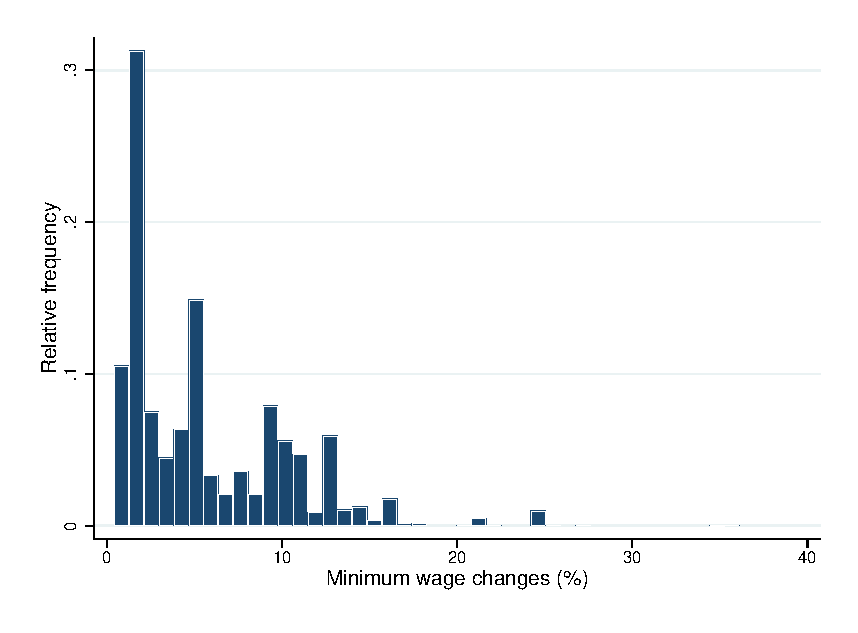
\includegraphics[width = \textwidth]
			{../../analysis/descriptive/output/pct_ch_mw_dist.eps}
	\end{subfigure}
	\begin{subfigure}{.49\textwidth}
		\caption{Timing}
		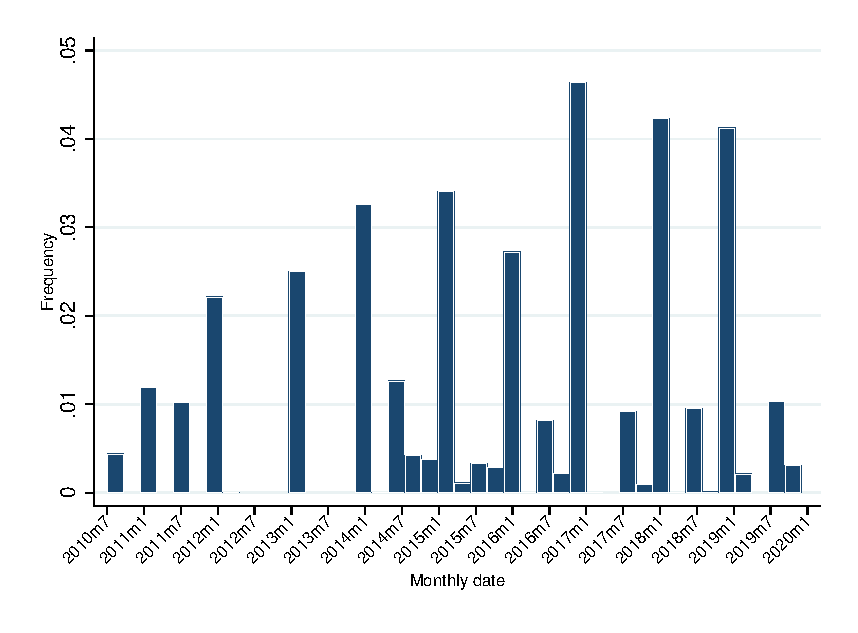
\includegraphics[width = \textwidth]
			{../../analysis/descriptive/output/pct_ch_mw_date_dist.eps}
	\end{subfigure}
	\begin{minipage}{.95\textwidth} \footnotesize
		\vspace{3mm}
		\textit{Notes:} The histograms show the distribution of positive MW changes 
		in the full sample of ZIP codes available in the Zillow data. Panel (a) reports 
		the intensity of the changes in percentage terms. Panel (b) plots the distribution 
		across time of such changes. 
	\end{minipage}
\end{figure}

We construct an alternative measure to capture the effects of MW policies: the 
\textit{experienced} MW. This measure aims to account for the fact that workplace location 
often differs from the residence one. The MW that matters for a given local rental market 
is the one experienced by the people living in it, and so by tracking where people in 
each ZIP code work we can get a better sense of the relevant MW there.

To construct this measure we need to know, for each ZIP code, where workers residing in 
that ZIP code work. We obtain this information from the 2017 Longitudinal Employer-Household 
Dynamics Origin-Destination Employment Statistics (LODES). In particular, we use the 
origin-destination matrix mapping jobs from residence to workplace locations. The data 
comes at the block group level. We aggregate that to construct a ZIP code residence-workplace 
matrix where we observe the number of workers for each residence-workplace pair.

We then use the ZIP code residence-workplace matrix to build exposure weights. Denote 
ZIP codes by $i$ and monthly dates by $t$. Let $\mathds{Z}_i$ be the set of ZIP codes in 
which $i$'s residents work (including $i$). We construct the set of weights 
$\{\omega_{iz}\}_{z \in \mathds{Z}_i}$ as $$\omega_{iz} = \frac{N_{iz}}{N_i} , $$ where 
$N_{iz}$ is the number of workers who reside in ZIP code $i$ and work in $z$, and $N_i$ 
is the total working population of ZIP code $i$.\footnote{The LODES data additionally 
	reports origin-destination matrices for number of workers 29 years old and younger  
	and number of workers earning less than \$1,251 per month. We compute weights based 
	on both these sub-groups as well. However, the resulting experienced MW measures with
	any set of weights are highly correlated among each other ($\rho>0.99$ for every pair).
	Thus, we use working population weights throughout the paper.} 
Given that origins present a large number of destinations with extremely low percentages of 
workers, we trim the number of destination ZIP codes to those making up to 90 percent of the 
workforce.\footnote{Results based on the full distribution are identical to those presented
	in the paper.} 
Letting $\underline{w}_{it}$ denote the statutory MW in ZIP code $i$ and month $t$, we 
define the experienced minimum wage measure as

\begin{equation}
	\underline{w}^{\text{exp}}_{it} = 
			\sum_{z \in \mathds{Z}_i} \omega_{iz} \underline{w}_{zt} \ . 
\end{equation}

The experienced MW of a ZIP code is based on the minimum wages binding in other ZIP codes 
where its residents work. An increase in a city, for example, may not have an impact on 
the local rental market if most residents are not minimum wage workers. It will, however, 
affect neighboring ZIP codes where MW workers reside. We will use this insight in our 
analysis. See \autoref{sec:emp_strategy_expmw} for some discussion on how we use this 
measure, and \autoref{sec:experienced_mw} for further details and estimation results.

%%%%%%%%%%%%%%%%%%%%%%%%%%%%%%%%%%%%%%%%%%%%%%%%%%%%%%%%%%%%%%%%%%%%%%%%%%%%%%%%%
\subsection{Other Data Sources}\label{sec:data/other_data}

We collect socio-demographic information from the 2010 Census and the 5-years 2008-2012 
American Community Survey (ACS). The data is initially obtained at the Census tract 
level and mapped into USPS ZIP codes using HUD crosswalks \parencite{hudCrosswalks}. We 
assign the following characteristics to each ZIP code: population, number of housing units, 
median income, African-American population, number of unemployed, and number of college 
students. We use this information to classify ZIP codes into, for example, high or low median 
income to then perform heterogeneity analysis.

To proxy for local economic activity we collect data from the Quarterly Census of 
Employment and Wages (QCEW) at the county-quarter and county-month level for each main 
industrial division.\footnote{The QCEW covers the following industrial aggregates: 
	``Agriculture, Forestry, and Fishing'', ``Mining'', ``Construction'', ``Manufacturing'', 
	``Transportation and Public Utilities'', ``Wholesale Trade'', ``Retail Trade'',
	``Financial activities'' (including insurance and real state), ``Services'', and 
	``Public Administration''.} 
For each county-quarter-industry cell, we observe the number of establishments and the 
average weekly wage. For each county-month-industry cell, we additionally observe the number 
of employed people. We merge this data onto our ZIP code-month panel by county and 
quarterly date.

%We add data from the \textit{Building Permit Survey} (BPS) at the county-month level to 
%account for time-varying shocks in the housing market. The BPS provides building permit 
%statistics on new privately-owned residential construction disaggregated by house type. 
%Lacking information on condos and cooperative houses, we only add the number of new units 
%and the permits valuation for single family houses to each ZIP code-month observation based 
%on the county and month they belong.

Finally, we use the LODES data to proxy for MW workers' residence and workplace location. 
Beyond the origin-destination matrices, the LODES data provides block-level information on 
jobs by residence area (RAC) and workplace area (WAC) characteristics. These include jobs 
for various types of workers.\footnote{LODES RAC and WAC datasets provide workers' breakdown 
	for the following characteristics: age (less than 29, 30 to 54, more than 55); workers' 
	earnings (less than \$1,251/mo., \$1,251/mo. to \$3,333/mo., more than \$3,333/mo.); 
	NAICS(11, 21, 22, 23, 31-33, 42, 44-45, 48-49, 51, 52, 52, 54, 55, 56, 61, 62, 71, 72, 
	81, 92); race (White alone, Black or African-American alone, American-Indian or Alaskan 	
	Native alone, Asian alone, Native Hawaiian alone, two or more race groups, not Hispanic 
	or Latino, Hispanic or Latino); educational attainment (less than high school, high 
	school or equivalent, some college or associate, bachelor's degree or advanced degree); 
	sex (male, female).} 
We use RAC and WAC datasets to ``locate" workers likely to earn MW by looking at the 
state-level distribution of such type of workers. We build, for each ZIP code in the sample, 
the share (out of the state total) of workers under 30 years old earning less than \$1,251 
per month that either \textit{live} or \textit{work} there. We take these data as 
time-invariant characteristics of our ZIP codes.


%%%%%%%%%%%%%%%%%%%%%%%%%%%%%%%%%%%%%%%%%%%%%%%%%%%%%%%%%%%%%%%%%%%%%%%%%%%%%%%%%
\subsection{The Resulting Panel}\label{sec:data_final_panel}

Using the data described above, we put together a panel dataset at the ZIP code and monthly 
date levels from February 2010 to December 2019. Given that ZIP codes enter the Zillow data 
progressively over time affecting the composition of the sample, we construct our baseline 
\textit{estimating panel} by keeping in the sample those ZIP codes with valid rents data as 
of July 2015.\footnote{We note that the resulting panel is still unbalanced, in the sense 
	that the time series for some ZIP codes starts before July 2015. However, from July
	2015 onward our data contains no missing values in the main rent variable used in the 
	analysis.} 
This panel contains 5,302 MW increases, which arise from 124 state changes and 99 county 
and local level changes. 4,224 of those changes take place after ZIP codes already entered
the panel, and thus are used in estimation.
%% See analysis/sumstats

We stress the fact that our data does not cover the full sample of ZIP codes, but rather a 
selected sample. Appendix \autoref{fig:maps} maps the full set of available 
ZIP codes in the Zillow data, together with population density. The Zillow sample seems 
fairly distributed across urban areas, although some important areas have limited coverage. 

\autoref{tab:desc_stats} further compares the Zillow sample to the population of ZIP codes 
along several critical demographic dimensions. Columns 1 and 2 report data for the whole 
universe of U.S. ZIP codes and for the top 100 U.S. metropolitan areas, respectively. In 
column 3 we show the complete set of ZIP codes in the Zillow data. Finally, column 4 shows 
our baseline estimating sample. Focusing on our preferred variable --median rent per square 
foot in the SFCC category--, we collect rent data from Zillow for 3,315 unique ZIP codes 
which amount to 8.5 percent of the 38,893 total for the entire U.S. and 46.7 percent 
of the 2010 U.S. population. 

The average median household annual income for those ZIP codes is \$65,475.2, almost 25 
percent higher than the same figure for the average U.S. ZIP code and 5 percent higher than 
the top 100 metropolitan areas. ZIP codes in the baseline sample are even richer, with an
average household income of \$69,919.7. Furthermore, both Zillow ZIP codes and those in our 
estimating panel have a higher share of urban population, college students, African-American
and hispanic population, and houses for rent than the average urban ZIP code. While Zillow
ZIP codes are likely are clearly different than the average urban location. In an attempt to 
capture the treatment effect for the average urban ZIP code we conduct an estimation 
re-weighting our sample to match characteristics of the top 100 CBSA sample of ZIP codes. 
Because our ZIP codes are richer than the average (i.e., arguably less influenced by MW
changes), we expect to find a larger effect in this exercise.

\begin{table}[h!]
	\caption{Descriptive Statistics of Different Sets of ZIP Codes}
	\centering
	\label{tab:desc_stats}    
	
% Table created by stargazer v.5.2.2 by Marek Hlavac, Harvard University. E-mail: hlavac at fas.harvard.edu
% Date and time: Thu, Nov 05, 2020 - 10:15:39 AM
\begin{tabular}{@{\extracolsep{5pt}} ccccc} 
\\[-1.8ex]\hline 
\hline \\[-1.8ex] 
 & U.S. & Top 100 CBSA & Full Panel & Est. Panel \\ 
\hline \\[-1.8ex] 
Population (millions) (2010) & $311.177$ & $189.712$ & $110.169$ & $50.619$ \\ 
Population as share of U.S. & $1$ & $0.610$ & $0.354$ & $0.163$ \\ 
Housing Units (millions) (2010) & $132.833$ & $78.738$ & $46.722$ & $21.323$ \\ 
Housing Units as share of U.S. & $1$ & $0.593$ & $0.352$ & $0.161$ \\ 
Urban Share (2010) & $0.464$ & $0.754$ & $0.958$ & $0.972$ \\ 
College Share (2010) & $0.464$ & $0.754$ & $0.958$ & $0.972$ \\ 
African-American Share (2010) & $0.464$ & $0.754$ & $0.958$ & $0.972$ \\ 
Hispanic Share (2010) & $0.097$ & $0.136$ & $0.173$ & $0.192$ \\ 
Elder Share (2010) & $0.150$ & $0.130$ & $0.124$ & $0.110$ \\ 
Poor Share (2010) & $0.464$ & $0.754$ & $0.958$ & $0.972$ \\ 
Unemployed Share (2010) & $0.089$ & $0.092$ & $0.092$ & $0.092$ \\ 
Mean HH income (2010) & $52,492.560$ & $62,773.640$ & $65,475.150$ & $66,919.730$ \\ 
Rent House Share (2010) & $0.295$ & $0.347$ & $0.381$ & $0.383$ \\ 
Work in same county share (2010) & $0.701$ & $0.684$ & $0.763$ & $0.756$ \\ 
Unique zipcodes & $38,893$ & $14,583$ & $3,315$ & $1,305$ \\ 
Share of state events & $$ & $$ & $0.030$ & $0.028$ \\ 
Share of county events & $$ & $$ & $0.001$ & $0.001$ \\ 
Share of  localevents & $$ & $$ & $0.003$ & $0.0005$ \\ 
Mean SFCC rent variable & $$ & $$ & $1.304$ & $1.269$ \\ 
Std. Dev. SFCC rent variable & $$ & $$ & $1.033$ & $0.827$ \\ 
Unique zipcodes SFCC rent variable & $$ & $$ & $3,316$ & $1,143$ \\ 
\hline \\[-1.8ex] 
\end{tabular} 

	\begin{minipage}{0.95\textwidth} \footnotesize
		\vspace{3mm} 
		\textit{Notes}: The table shows characteristics of four sets of U.S. postal service 
		ZIP codes. Column 1 reports demographic statistics for the universe of USPS ZIP code 
		we were able to map. Column 2 shows the same statistics for for the top 100 Core-Based 
		Statistical Areas (CBSA). Column 3 shows the characteristics of the set of ZIP codes 
		available in the Zillow data. Finally, column 4 shows the restricted balanced sample 
		we use as baseline in our empirical analysis. All demographic information comes from 
		the 2010 Census and the 5-years 2008-2012 ACS.
	\end{minipage}
\end{table}

Finally, \autoref{tab:estimating_panel_stats} shows some basic sample statistics of our 
baseline estimating panel. As suggested in the table, the statutory and experienced MW 
are quite similar. We compare these measures in more detail in \autoref{sec:experienced_mw}.
We also show summary statistics of median rents in the SFCC category. The average of 
monthly median rents is \$1,651 in absolute values and \$1.27 per square foot, although 
these variables show a great deal of variation. Finally, for illustration, we show average 
weekly wage, employment and establishment-count for the ``Financial activities'' sector 
from the QCEW. Appendix \autoref{tab:estimating_panel_stats_long} additionally shows 
summary statistics for the experienced MW computed using alternative weights, rents in 
different categories of the Zillow data, and the full set of QCEW industries we use as 
controls in our regressions.

\begin{table}[h!]
	\caption{Descriptive Statistics of Estimating Panel}
	\centering
	\label{tab:estimating_panel_stats}    
	
% Table created by stargazer v.5.2.2 by Marek Hlavac, Harvard University. E-mail: hlavac at fas.harvard.edu
% Date and time: Fri, Dec 11, 2020 - 1:50:17 PM
\begin{tabular}{@{\extracolsep{5pt}}lccccc} 
\\[-1.8ex]\hline 
\hline \\[-1.8ex] 
Statistic & \multicolumn{1}{c}{N} & \multicolumn{1}{c}{Mean} & \multicolumn{1}{c}{St. Dev.} & \multicolumn{1}{c}{Min} & \multicolumn{1}{c}{Max} \\ 
\hline \\[-1.8ex] 
Statutory MW & 155,295 & 8.08 & 1.21 & 7 & 16 \\ 
Experienced MW & 155,295 & 8.06 & 1.21 & 6.29 & 14.98 \\ 
Median rent psqft. SFCC & 113,375 & 1.27 & 0.83 & 0.47 & 7.25 \\ 
Median rent SFCC & 125,644 & 1,651.10 & 702.99 & 595.00 & 6,595.00 \\ 
Avg. wage Fin. activities & 151,032 & 1,561.71 & 961.88 & 0.00 & 9,557.00 \\ 
Employment Fin. activities & 151,032 & 59,595.23 & 75,840.23 & 0.00 & 397,839.00 \\ 
Estab. count Fin. activities & 151,032 & 5,105.58 & 5,201.89 & 31.00 & 30,405.00 \\ 
\hline \\[-1.8ex] 
\end{tabular} 

	\begin{minipage}{0.95\textwidth} \footnotesize
		\vspace{3mm} 
		\textit{Notes}: The table shows descriptive statistics of our baseline estimating panel.
		Variables included are the statutory and experienced MW, constructed as explained in
		\autoref{sec:mw_construction}; the average of median monthly rents per square foot and 
		total in the SFCC category, taken directly from Zillow; and average weekly wage, employment 
		and establishment count in the Financial Sector from the QCEW.
	\end{minipage}
\end{table}


\section{Empirical Strategy}\label{sec:empirical_strategy}
    %%%%%%%%%%%%%%%%%%%%%%%%%%%%%%%%%%%%%%%%%%%%%%%%%%%%%%%%%%%%%%%%%%%%%%%%%%%%%%%%%
%%%%%                         EMPIRICAL STRATEGY                             %%%%
%%%%%%%%%%%%%%%%%%%%%%%%%%%%%%%%%%%%%%%%%%%%%%%%%%%%%%%%%%%%%%%%%%%%%%%%%%%%%%%%%
    
%%%%%%%%%%%%%%%%%%%%%%%%%%%%%%%%%%%%%%%%%%%%%%%%%%%%%%%%%%%%%%%%%%%%%%%%%%%%%%%%%
\subsection{First-differences model}

Consider the following two-way fixed effects model relating rents and the 
minimum wage:
\begin{equation*} \label{eq:did_lev}
    r_{it} = \alpha_i + \hat{\delta}_t 
           + \gamma \mw^{\res}_{it} + \beta \mw^{\wkp}_{it}
           + \mathbf{X}^{'}_{it}\eta
           + \varepsilon_{it} \ 
\end{equation*}    
where
$i$ and $t$ index ZIP codes and time periods (months),
$r_{it}$ represents the log of rents per square foot,
$\mw^{\res}_{it}$ is the ZIP code's residence MW, defined as 
$\ln \MW_{it}$,
$\mw^{\wkp}_{it}$ is the ZIP code's workplace MW, defined as 
$\sum_{z\in\Z(i)} \pi_{iz}\ln \MW_{zt}$,
$\alpha_i$ and $\hat{\delta}_t$ are fixed effects, and 
$\mathbf{X}_{it}$ is a vector of county-level time-varying controls.
Time runs from February 2010 ($\underline{T}$) to December 2019 ($\overline{T}$).
The parameters of interest are $\gamma$ and $\beta$, which we interpret as the 
elasticity of rents to the residence and workplace MW, respectively.

By taking first differences on the previous equation we obtain
\begin{equation}\label{eq:fd}
    \Delta r_{it} = \delta_t
                  + \gamma \Delta \mw^{\res}_{it} + \beta \Delta \mw^{\wkp}_{it}
                  + \Delta \mathbf{X}^{'}_{it}\eta
                  + \Delta \varepsilon_{it} ,
\end{equation}
where $\delta_t = \hat{\delta}_t - \hat{\delta}_{t-1}$.
We spell out the model in first differences because it is reasonable to expect 
unobserved shocks to rental prices to be persistent over time. 
Appendix Table XX shows evidence of AR(1) auto-correlation in the error term.
% SH: 
%    Add Woldrige cite in the notes of table \textcite[][chapter 10]{wooldridge2010}
The main results of the paper are obtained under the model in \ref{eq:fd}. 
However, to compare to previous results we also estimate versions of the model
that exclude some of the MW measures.



%%%%%%%%%%%%%%%%%%%%%%%%%%%%%%%%%%%%%%%%%%%%%%%%%%%%%%%%%%%%%%%%%%%%%%%%%%%%%%%%%
\subsection{Identification and Causality}

We start by noting that, in order to separately identify the effect of 
residence and workplace MW changes, we need these variables to have independent
variation.
While this requirement is standard, it is not obvious that it holds in our
application.
For instance, if there were a single national minimum wage level or if everybody 
lived and worked in the same location, then we would have
$\Delta \mw^{\res}_{it} = \Delta \mw^{\wkp}_{it}$ for all $(i,t)$.
In the next section we show that there is substantial independent variation
in the MW measures.

Being able to compute $\gamma$ and $\beta$ does not mean that they can be given
a causal interpretation.
For this, we require a \textit{strict exogeneity} of both MW variables.
Formally,
\begin{equation*}\label{eq:strict_exogeneity}
    E\left[
        \begin{pmatrix}
            \Delta \mw^{\res}_{is} \\
            \Delta \mw^{\wkp}_{is} \\
        \end{pmatrix}
        \Delta \varepsilon_{it}
    \bigg| \delta_t, \Delta \mathbf{X}_{it} \right] =
    \begin{pmatrix}
        0 \\
        0 \\
    \end{pmatrix}
\end{equation*}
for all $s\in\{\underline{T}, ..., \overline{T}\}$.
That is, we require the unobserved shocks to rents to be uncorrelated with 
past and present values of changes in our MW measures 
conditional on time-period fixed effects and controls.

This assumption has two important implications.
First,
it implies no pre-trends in rents leading up to minimum wage changes 
(conditional on controls). We will test this implication more formally by 
including leads of the MW variables.
Second,
it rules out feedback effects from current values of rents on our MW variables, 
i.e., MW changes are assumed not to be influenced by past values of rents.
While we think this is a reasonable assumption---MW levels are usually not 
set by considering their effects on the housing market---, we allow this type of 
feedback effects in a specification described in the upcoming subsection.
Finally, we note that our identifying assumption allows for arbitrary 
correlation between ZIP code effects $\alpha_i$ and both MW variables
(e.g., our empirical strategy is robust to the fact that richer districts tend 
to vote for MW policies).


We worry that unobserved shocks, such as local business cycles, may 
systematically affect both rents and minimum wage changes, which is why
we include period-fixed effects and time-varying controls.
The period fixed effects should capture common trends in the housing market.
In some specifications we allow this trends to vary by CBSA.
To control for variation arising from unobserved trends in local markets we 
include economic controls from the QCEW.%
\footnote{These data are aggregated at the county level, and represent a second best given the 
unavailability of controls at the ZIP code level.}
Specifically, we use average weekly wages, employment and establishment counts 
for the sectors ``Professional and business services,'' ``Information,'' and 
``Financial activities.''
We assume that these sectors are not affected by the minimum wage.
In fact, according to \textcite[][table 5]{MinWorkersReportBLS}, in 2019 
such industries accounted for 3.5, 1, and 1.2 percent of the total number of MW workers, 
respectively.%
\footnote{In Appendix \ref{sec:app_econ_control} we show suggestive evidence 
that they are not affected by the MW by using them as dependent variable in our 
models.}
%%% SH:
%%%    REVISE APPENDIX
We also try models where we control for ZIP code-specific linear and quadratic 
trends, which should account for time-varying heterogeneity not captured by our 
economic controls that follows this pattern.

We can test the identification assumption using models that include leads and lags
of the MW variables:
\begin{equation} \label{eq:leads_lags}
    \Delta r_{it} = \delta_t
                  + \sum_{r=-s}^{s} \gamma_s \Delta \mw^{\res}_{is} 
                  + \sum_{r=-s}^{s} \beta_s \Delta \mw^{\wkp}_{is}
                  + \Delta \mathbf{X}^{'}_{it}\eta
                  + \Delta \varepsilon_{it} ,
\end{equation}
where $s$ is the number of months of a symmetric window around the MW change. 
We use $s=6$ but our results are very similar for windows of 3 or 9 months.
Because the MW measures are strongly correlated, adding leads and lags of both 
leads to a decline in precision.
Thus, we try models with leads and lags of only one of the MW measures as well.

Under the assumption that there are no anticipatory effects in the housing 
market, we interpret the absence of pre-trends as evidence against the presence 
of unobserved economic shocks driving our results.\footnote{We can also interpret the absence of pre-trends as a test 
	for anticipatory effects if we are willing to assume that the controls embedded in 
	$\mathbf{X}^{'}_{ct}$ capture all relevant unobserved heterogeneity arising from local 
	business cycles. While we find the interpretation given in the text more palatable, the 
	data does is consistent with both.}
    We think that, given the high frequency of our data and that we focus on short windows around MW 
    changes, the assumption of no anticipatory effects is reasonable. We further present evidence in 
    favor of this assumption by showing that MW changes do not predict the number of listings of 
    houses for sale in Zillow.\footnote{Ideally, we would run this regression on the number of rental 
        units. Unfortunately, as described in Section \ref{sec:data}, this information is not available.}
    Specifically, we can track the number of houses listed for sale in selected ZIP codes during the 
    period 2013-2019 for our preferred house type (SFCC). We use such series to run placebo 
    regressions where we estimate both the static and dynamic models using the change in (log) 
    listings as dependent variable. %Significant effects of MW changes, or pronounced pre-trends will 
    %indicate that policy changes actually affect the Zillow inventory composition and cast doubt on
    %the identifying assumption. We fail to find that.




The model in \ref{eq:fd} assumes a balanced panel of ZIP codes.
However, as explained in Section XX   %% Refer to last part of data section
we use a partially balanced panel.

%%%%%%%%%%%%%%%%%%%%%%%%%%%%%%%%%%%%%%%%%%%%%%%%%%%%%%%%%%%%%%%%%%%%%%%%%%%%%%%%%
\subsection{Identification beyond the MW measures}

Appendix \ref{sec:did_spillovers_id} shows that under parallel trends assumptions
the model in equation \ref{eq:fd} identifies parameters $\gamma$ and $\beta$.


%%%%%%%%%%%%%%%%%%%%%%%%%%%%%%%%%%%%%%%%%%%%%%%%%%%%%%%%%%%%%%%%%%%%%%%%%%%%%%%%%
\subsection{Alternative models}


Inspired by this approach, we use a stacked sample in Appendix Table XX.

Appendix Table XX shows that we obtain similar results under a weaker 
\textit{sequential exogeneity} assumption \parencite{ArellanoHonore2001}.
%% SH: 
%%    Discuss estimation procedure in notes of figure


\section{Results}\label{sec:results}
    %%%%%%%%%%%%%%%%%%%%%%%%%%%%%%%%%%%%%%%%%%%%%%%%%%%%%%%%%%%%%%%%%%%%%%%%%%%%%%%%%
%%%%%                                RESULTS                                 %%%%
%%%%%%%%%%%%%%%%%%%%%%%%%%%%%%%%%%%%%%%%%%%%%%%%%%%%%%%%%%%%%%%%%%%%%%%%%%%%%%%%%

In this section we present our main results. Initially, we use the \textit{static} model
to estimate an elasticity of the MW to rents of about 0.026 (s.e. 0.013). We check the
robustness of our results by progressively including plausible controls for the dynamics 
of the local economy, and by including parametric local trends. Our results do not change.

Following the reasoning in \autoref{sec:empirical_strategy}, we then present estimates of 
\textit{dynamic} models. Results show a short-lived dynamic effect, mainly over the two
months following the policy: we estimate the cumulative impact of a 10 percent MW increase 
to be between 0.5 and 0.6 percent over the course of the 5 months after the policy change. 
We find no pre-trends in our estimations, which under the assumption of fixed housing supply 
we interpret as evidence in favor of our identification assumption. We indirectly assess the 
validity of the housing supply assumption by running a placebo regression where we replace 
our main dependent variable with the number of listings \textit{for sale} in Zillow. 
Finally, we estimate panel models that include the lagged dependent variable as control,
which deliver a similar long run effect.

% SH: I removed the below. I don't think we need into that much detail in this overview

%, where we don't find any significant effect.\footnote{This exercises implicitly assumes 
%the presence of of a correlation between the number of listings \textit{for rent} and 
%\textit{for sale} on Zillow.}


% SH: I removed references to particular subsections. I'm happy to include those, but we have to be
% consistent. If we decide to do that we should reference all subsections.

% SH: Following Jesse's comments, I removed the comment on how our main estimate can be seen as 
% a lower bound from the paragraph below

We conduct two exercises to assess to what extent our results estimated in the Zillow sample 
are representative of the underlying average treatment effect across the population of urban
zipcodes. First, we re-estimate our static model via weighted regression, where weights for 
each zipcode are constructed so that our sample matches demographic statistics of the top 100 
CBSA.  As expected, we find that the estimated elasticity increases slightly. Second, we 
re-estimate our static model on a expanded sample that includes the whole set of zipcodes 
available in the Zillow data, no matter the data they ``entered'' the panel. We account for 
changes in zipcode composition by controlling for entry cohort $\times$ time fixed effects. 
Our results show robust to this exercise.

% SH: I removed references to experienced MW below, which will go in the experienced_MW section
%     I also removed discussion of the benchmarking

After establishing the robustness of our results, we follow the strategy outlined in 
\autoref{sec:strategy_heterogeneity} to investigate how the incidence of the effect may vary 
across the distribution of zipcode characteristics. First, we use LODES data to proxy for MW 
workers residence and workplace location to show how effects disproportionately affect those 
zipcode that are more likely to have low-wage workers as residents. Secondly, we estimate the 
heterogeneous impact of MW changes across the distribution of several census-based 
demographics. The results indicate that the effects are concentrated in poorer, less-educated, 
and more African-American zipcodes. 

Importantly, all regressions cluster standard errors at the state level so to match the main 
source of variation of MW changes.

%%%%%%%%%%%%%%%%%%%%%%%%%%%%%%%%%%%%%%%%%%%%%%%%%%%%%%%%%%%%%%%%%%%%%%%%%%%%%%%%%
\subsection{Baseline Results}\label{sec:baseline_results}

\autoref{tab:static_model} presents results from the static model defined in \autoref{eq:did}. In 
column 1, we show the classical two-way fixed effects model --zipcode and monthly date--, 
estimated in first differences. A potential threat to the identification is the presence of 
unobserved shocks systematically affecting MW and rent changes. In order to account for this 
possibility, in columns 2 to 5 we show results of several models with different sets of controls 
that proxy for shocks to the local economy in columns 2, 3, and 4. As we discussed in the previous 
section, the controls are taken from the QCEW and thus vary either at the county-month or 
county-quarter level. While this prevents us from studying the presence of time-varying 
confounding factors at the zipcode-level, the controls plausibly capture shocks correlated with 
MW changes, which are also decided at higher levels of aggregation than the zipcode --i.e., city, 
county, or state levels. In fact, if there are underlying factors affecting MW changes that also 
affect zipcode-level rents, they would likely arise from this larger geographic units. 

Wages, employment and the number of establishments are also potentially affected by MW changes,
which may result in an invalid regression due to the use of ``bad controls'' 
\parencite{AngristPischke2009}. To avoid this problem we only include controls from industries 
that are unlikely to be affected by MW policies. These are ``Professional and Business Services", 
%% UPDATE SECTORS AFTER REVIEW
``Information", and ``Financial activities". The controls used in the regression are as follows:
column 2 includes average weekly wages at the county-quarter level; column 3 controls for 
employment at the county-month level; column 4 uses the number of establishments in the 
corresponding county and quarter. We include the difference in the log of each variable in our
regressions. Finally, in column 5 we jointly account for all sets of controls. All specifications 
return very similar results. A 10 percent increase in the MW leads to a 0.26 percent increase 
in rents. 

One may still worry that heterogeneous dynamics in local markets at the zipcode level bias our 
results. To account for that, \autoref{tab:did_trend} in the appendix reports estimation 
results of the static model that include zipcode-specific linear and quadratric trends as controls. 
Reassuringly, the coefficient of interest does not change.

\begin{table}[h!]
    \caption{The static effect of MW increases on rents}
    \label{tab:static_model}
    \centering
    {
\def\sym#1{\ifmmode^{#1}\else\(^{#1}\)\fi}
\begin{tabular}{l*{3}{c}}
\hline\hline
          &\multicolumn{1}{c}{(1)}&\multicolumn{1}{c}{(2)}&\multicolumn{1}{c}{(3)}\\
          &\multicolumn{1}{c}{D.ln\_med\_rent\_psqft}&\multicolumn{1}{c}{D.ln\_med\_rent\_psqft}&\multicolumn{1}{c}{D.ln\_med\_rent\_psqft}\\
\hline
D.ln\_mw   &   0.0260\sym{**} &   0.0257\sym{**} &   0.0255\sym{**} \\
          & (0.0128)         & (0.0120)         & (0.0117)         \\
\hline
Zipcode-specifc linear trend&       No         &      Yes         &      Yes         \\
Zipcode-specific linear and square trend&       No         &       No         &      Yes         \\
R-squared &    0.022         &    0.024         &    0.026         \\
Observations&   112232         &   112232         &   112232         \\
\hline\hline
\end{tabular}
}

    \begin{minipage}{0.9\textwidth} \footnotesize
		% UPDATE NOTES
		\vspace{3mm} 
		\textit{Notes}: The table reports coefficients from versions of \autoref{eq:did} 
		estimated on the balanced panel of zipcode-months described in \autoref{sec:data}. 
		The dependent variable is the difference in the natural logarithm of median	rents 
		per square foot in the Single Family, Condos and Condominiums category in Zillow, 
		whereas the main independent variable is the difference in the natural logarithm of 
		the statutory minimum wage. All columns control for monthly date fixed effects. In 
		addition, columns (2) to (5) include economic controls from the industries 
		%%% UPDATE SECTORS AFTER REVIEW
		``Professional and business services'', ``Information'', and ``Financial activities'' 
		from the QCEW. Wage controls are the difference in the natural logarithm of average 
		weekly wages, employment controls are the difference in the natural logarithm of 
		employment, and establishment count controls refer to the difference in the natural 
		logarithm of number of establishments. Wages and establishment count vary at the 
		county-quarter level, whereas employment varies at the county-month level. Standard 
		errors are clustered at the state level. Significance codes: *** $p < 0.01$, ** 
		$p < 0.05$, * $p < 0.1$.
	\end{minipage}
\end{table}

A causal interpretation of the estimates from the static model relies on a \textit{strict exogeneity} 
assumption, which states that minimum wage changes are orthogonal to past and future changes in rents.
This assumption may not hold in practice. One way to assess its validity is by a classical 
``pre-trends test''. To conduct that test we estimate a dynamic model with leads and lags of MW 
changes, and evaluate whether coefficients on leads are zero. Under the assumption that the MW does 
not affect the supply of rentals, economic shocks leading to both increases in the MW and rents would 
show up as non-zero pre-trends. A second problem with the strict exogeneity assumption, although a less 
concerning one, is that it presupposes no dynamic effect of MW changes. This restriction is eased by 
the inclusion of lags in the model.

In \autoref{fig:dynamic_models_main}, we plot the estimated coefficients of the \textit{dynamic} model 
(including the full set of economic controls) together with 90\% confidence intervals. In the 
appendix (\autoref{tab:dynamic_lags_leads_main}) we show the full set of coefficients, fit 
statistics, and a p-value of an F-test of the hypothesis that all leads are jointly equal to zero, 
for models with varying sets of controls. The confidence intervals of the pre-trend coefficients in 
\autoref{fig:dynamic_model_coeffs} always include zero. Furthermore, as shown in the appendix we 
always fail to reject the hypothesis of no pre-trends. Consistent with a causal interpretation of 
our results, future MW changes do not have an effect on current rental prices. 

We stress that this interpretation relies on the assumption that the supply of rental units is 
not affected by MW changes. Given the high-frequency of our data, we believe this assumption is 
likely to hold. We provide indirect evidence of this assumption in the appendix  
(\autoref{fig:placebo_nlist}), where we estimate our main dynamic model on the number of listings 
\textit{for sale} in Zillow. The results, although somewhat noisy, suggest that MW changes not 
affect the number of listings for sale in Zillow. Because this variable is likely to be correlated 
with the number of rentals, we see this result as evidence in favor of the assumption of fixed supply. 
The supply of rentals, however, may also be affected by the MW in terms of its quality. For instance, 
it is possible that the quality of houses in Zillow increases after a MW increase, leading to a 
spurious rise in their price.  Unfortunately, due to data limitations we are not able to study this 
possibility. Our results then hinge on the assumption that quality of rental units is not affected 
by the MW.

The strict exogeneity assumption seems to be failing with respect to the lags. Our dynamic model 
captures a short-lived persistence of the effect of MW changes on rents. Following a 10 percent 
change in the MW, we estimate that rents increase by 0.26 in the same month and 0.15 percent in the 
month \textit{after} the change, while the impact appears to vanish after the first two periods. 
\autoref{fig:dynamic_model_cumsum} shows the cumulative sum of the coefficients in the dynamic model,
together with 90\% confidence bands. The cumulative effects seems to stabilize after a significant 
increase in the period of the MW increase and the following one. \autoref{tab:dynamic_lags_leads_main}
reports a cumulative sum of coefficients for our preferred model with the full set of controls 
of 0.058 (s.e. 0.034), meaning that a 10 percent rise in the MW leads to a 0.58 percent increase 
in rents after 5 months.
%%% REVIEW EXACT NUMBERS AFTER CHANGING CONTROLS

Given that our models are not designed to estimate the long-run effect of the policy, we see the
standard errors on the cumulative effect as excessively large. The first attempt to obtain a more
precise estimate of this quantity is to estimate a dynamic model including distributed lags only. 
\autoref{fig:dynamic_models_main} shows such a model alongside the fully dynamic one. The top panel 
shows that the coefficients on lags are almost identical in this model, whereas the bottom panel 
suggests the cumulative effect follows a similar pattern, but in this case with slightly tighter 
confidence bands. A second way to obtain a more precise estimate of the long-run effect is by the 
panel specification in \autoref{eq:ab_panel}. In such a model, the long-run effect can be estimated 
as a non-linear transformation of three coefficients. \autoref{fig:dynamic_model_cumsum} shows such 
an estimate, which has a nearly identical magnitude but a considerably smaller confidence interval.
We report exact values for this estimate in \autoref{tab:horse_race_ab} in the appendix.

As we discussed before, the advantages of panel specifications go beyond computing a long-run effect.
This model accounts for the possibility that auto-correlation in the dependent variable bias our 
estimates. Furthermore, the identification in the panel model is valid under a weaker assumption on 
the relation between MW and rents changes: sequential exogeneity. \autoref{tab:horse_race_ab} in the 
appendix shows complete results for panel specifications alongside our main dynamic models. Columns 1, 
2, and 3 show coefficients from equations the static, dynamic, and lags only model respectively. Columns 
4 and 5 show results of panel specifications with and without leads. We recover the coefficients via 
instrumental variables following the well-known \textcite{ArellanoBond1991} approach, i.e., by using 
deeper lags of the dependent variable to instrument for the lagged dependent variable. Reassuringly, 
the estimated coefficients on leads and lags of our MW variable are very similar between the dynamic
and panel models. We interpret this result as rendering supporting our main identification assumptions
in the dynamic model. Focusing on the lags only model, we estimate a highly significant auto-correlation 
coefficient in the rents variable of 0.43. The implied long-run effect is 0.06 (s.e. 0.024).

\begin{figure}[htb!]
    \caption{The dynamic effects of MW increases on rents}
    \label{fig:dynamic_models_main}
    \centering
    \begin{subfigure}[b]{0.7\textwidth}
    	\caption{Coefficients}
    	\label{fig:dynamic_model_coeffs}
    	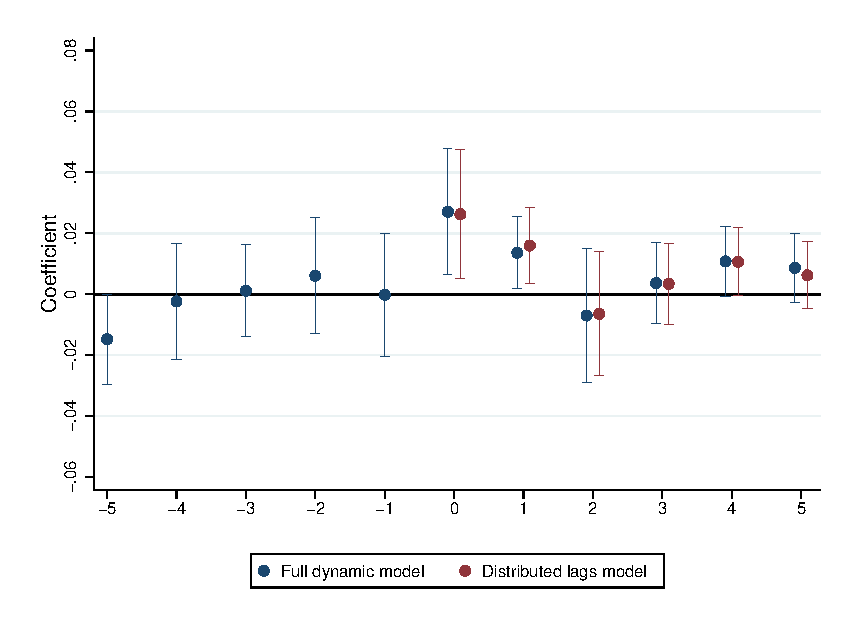
\includegraphics[width = \textwidth]
    	{../../analysis/first_differences/output/fd_models_coeffs_w5.eps}
    \end{subfigure}
    \begin{subfigure}[b]{0.7\textwidth}
    	\caption{Cumulative sum}
    	\label{fig:dynamic_model_cumsum}
    	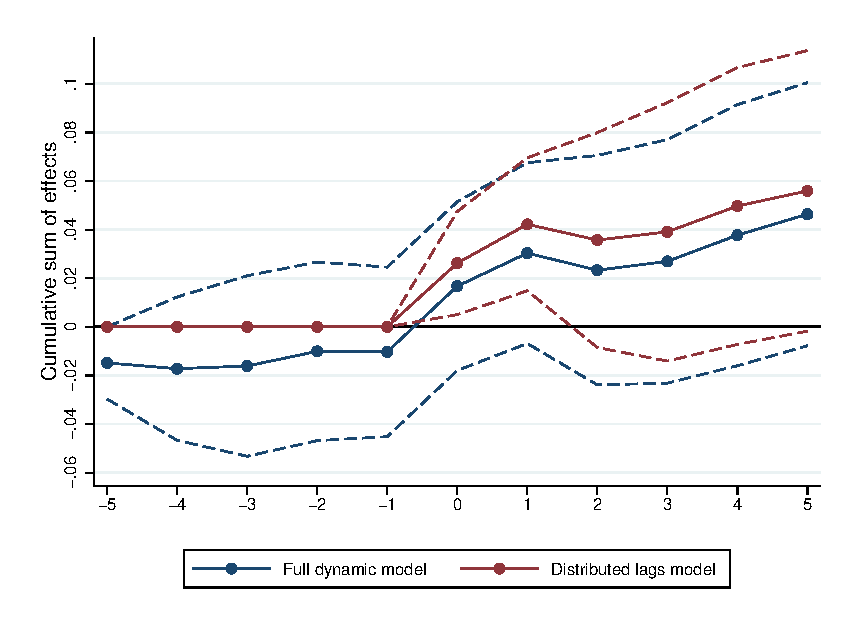
\includegraphics[width = \textwidth]
    	{../../analysis/first_differences/output/fd_models_cumsum.eps}
    \end{subfigure}
    \begin{minipage}{0.95\textwidth} \footnotesize
		\vspace{2mm} 
		\textit{Notes}: Panel (a) shows the estimated coefficients of the dynamic model defined in 
		equation \autoref{eq:leads_lags}, together with a distributed lags model that sets pre-event 
		coefficients to zero. Panel (b) shows the cumulative effect of the coefficients reported in 
		panel (a) for the same specifications. In addition, panel (b) includes the long-run effect 
		derived from the panel specification in \autoref{eq:ab_panel}. Complete results for the 
		dynamic model are reported in \autoref{tab:dynamic_lags_leads_main}, whereas results for the 
		distributed lags and panel models are reported in \autoref{tab:horse_race_ab}. 
		All models control for monthly date fixed effects. All models additionally  
		include economic controls from the industries ``Professional and business services'', 
		``Information'', and ``Financial activities'' from the QCEW. Wage controls are 
		the difference in the natural logarithm of average weekly wages, employment 
		controls are the difference in the natural logarithm of employment, and 
		establishment count controls refer to the difference in the natural logarithm 
		of number of establishments. Wages and employment vary at the county-month level,
		whereas establishment count varies at the country-quarter level. Both panels
		show 90 percent confidence intervals for the estimates, clustered at the state level. 
	\end{minipage}
\end{figure}


%%%%%%%%%%%%%%%%%%%%%%%%%%%%%%%%%%%%%%%%%%%%%%%%%%%%%%%%%%%%%%%%%%%%%%%%%%%%%%%%%
\subsection{Sample Selection Concerns and External Validity}\label{sec:sample_rest}

Our results suggest a noticeable impact of MW policies on the rental housing market. However, as 
explained in \autoref{sec:data}, the set of zipcodes for estimation constitutes a sample of, on 
average, more urban and richer zipcodes. This, in turn, may imply that our estimated effect has 
limited validity in other places. Additionally, the zipcodes included in the final sample are the 
ones appearing earlier in the Zillow data (i.e. zipcodes whose rent data are available since July 
2015). The zipcodes selected into the sample by this rule may differ from the average zipcode 
in unobservable dimensions that affect our results. In this section we conduct two exercises to 
test the sensitivity of our results to our sample.

First of all, we estimate our model on an \textit{unbalanced} panel of zipcodes, constructed by 
extending our panel to include the full set of zipcodes for which there is available rent data in 
Zillow. This, on one hand, doubles the sample size and increases significantly the number of MW 
events. %% SH: By how much? Make some numbers
On the other hand, as we now include zipcodes whose entry date to the panel is any month between
2010 and 2019, this procedure makes the composition of our sample vary strongly over time by. To 
account for the fact that zipcodes entering the panel in different dates may experience different 
dynamics, we estimate our models with controls for ``cohort'' $\times$ monthly date fixed effects. 
As a result, our regressions compare treated and untreated zipcodes conditional on length of their 
data.

Secondly, we assess the representativeness of our estimates by re-weighting zipcodes so as to match 
socio-demographic characteristics of the zipcodes in the top-100 CBSA. We do this by applying the 
entropy balancing procedure developed by \cite{hainmueller2012entropy} on the following zipcode 
level demographics: share of rental houses, share of African-American residents, share of college 
graduates, and median income. We target averages from \autoref{tab:desc_stats}, column 
2.\footnote{The entropy balancing procedure consists of a re-weighting scheme that assigns a scalar 
	weight to every unit such that the re-weighted sample matches moments of a target population. 
	Our implementation uses the \texttt{STATA} package \texttt{ebalance}, described in 
	\textcite{hainmueller2013ebalance}.} 
Armed with the set of weights, we re-estimate our models via weighted regression.

In \autoref{tab:wgt_unbal_comparison} we compare baseline results with those obtained from the 
two exercises. For each specification, we show the estimated impact from the static model, the 
cumulative effect obtained from the distributed lags model, and the long-run effect computed after
IV estimation of a distributed lags panel model. Column 3 shows the results obtained from 
estimating weighted models. The point estimate is now over 50\% higher, although the confidence 
interval includes the point estimate of the baseline model. The reweighted model suggests that the 
average effect of a 10 percent increase in MW is a 0.39 percent increase in same-month rents, 0.73 
percent after 5 months according to the dynamic model, and 0.69 in the long-run according to our 
panel specification. We interpret this as suggestive evidence that, in our selected sample of 
richer than average zipcodes, the effect of MW increases tends to be smaller. Column 2 shows that 
using the unbalanced panel results in slightly lower estimates. In particular, the panel 
specification is not estimated very precisely, resulting in a statistically non-significant 
long-run effect. This can be in part explained by the fact that these models include many more 
fixed effects, although it also suggests that zipcodes that entered earlier to our data experience 
somewhat larger impacts of MW changes.

In addition, \autoref{fig:dynamic_wgt_unabl_comp} in the Appendix shows the coefficients and 
cumulative sum from our dynamic models. Both panels show a remarkably similar pattern when compared 
to \autoref{fig:dynamic_models_main}. The reweighted and unbalanced model both show an absence of 
pre-trends, as well as a two-months dynamic effect following a MW increase.


\begin{table}[h!]\centering
	\caption{Robustness of the main estimates to sample selection}  %% Can you improve this name?
	\label{tab:wgt_unbal_comparison}
	{
\def\sym#1{\ifmmode^{#1}\else\(^{#1}\)\fi}
\begin{tabular}{l*{3}{c}}
\hline\hline
          &\multicolumn{1}{c}{(1)}&\multicolumn{1}{c}{(2)}&\multicolumn{1}{c}{(3)}\\
          &\multicolumn{1}{c}{Baseline}&\multicolumn{1}{c}{Reweighted}&\multicolumn{1}{c}{Unbalanced}\\
\hline
Static Effect&   0.0257\sym{**} &   0.0389\sym{***}&   0.0225\sym{*}  \\
          & (0.0124)         & (0.0131)         & (0.0115)         \\
\hline
\vspace{-1mm}&                  &                  &                  \\
Cumulative effect&0.06\sym{*}         &0.074\sym{*}         &0.053\sym{*}         \\
          &  (0.034)         &  (0.043)         &   (0.03)         \\
\hline    &                  &                  &                  \\
Wage controls&      Yes         &      Yes         &      Yes         \\
Employment controls&      Yes         &      Yes         &      Yes         \\
Establishment-count controls&      Yes         &      Yes         &      Yes         \\
R-squared &    0.022         &    0.023         &    0.053         \\
Observations&  107,781         &  107,781         &  182,608         \\
\hline\hline
\end{tabular}
}

	\begin{minipage}{0.95\textwidth}\footnotesize
	\vspace{3mm}	
	\textit{Notes:} The table reports estimations of the static, dynamic model with distributed
	lags only, and panel specification with distributed lags only discussed in 
	\autoref{sec:empirical_strategy}. The first column uses the baseline sample of zipcodes. The 
	second column uses the baseline sample reweighted so as to match moments of the overall 
	distribution of U.S. urban zipcodes, as explained in the text. The third column uses an 
	unbalanced 	panel constituted of the full set of zipcodes reported in the Zillow data. The 
	first row reports the main coefficient of the static model. The second row reports the 
	cumulative sum of the dynamic coefficients from the dynamic model with distributed lags only. 
	The third row reports the long-run effect from the panel specification, computed as specified 
	in the text. All specifications include time fixed effects, and additionally use QCEW data to 
	control for wages, employment and number of establishments for the ``Professional and business 
	services", ``Information", and ``Financial activities" industries. The number of observations 
	correspond to the ones used in the dynamic models. Standard errors are clustered at the state 
	level. Significance codes: *** $p < 0.01$, ** $p < 0.05$, * $p < 0.1$.	
	\end{minipage}
\end{table}



%%%%%%%%%%%%%%%%%%%%%%%%%%%%%%%%%%%%%%%%%%%%%%%%%%%%%%%%%%%%%%%%%%%%%%%%%%%%%%%%%
\subsection{The Heterogeneous Impact of MW Changes on Rents}\label{sec:heter}

Our baseline results in this section documented a significant effect of changes in the MW
on changes in rents per square foot. We argued that, given some reasonable assumptions on the 
behavior of unobservables, this effect can be interpreted casually. Furthermore, we provided
suggestive evidence in favor of those assumptions and discussed alternative assumptions 
that yield similar results (the panel specification). We showed in robustness exercises that 
our results persist under different samples, and that the average treatment effect for the 
universe of urban zipcodes in the U.S. is likely larger than the one in our selected sample. 


In this subsection we explore how the effect varies across the distribution of observable 
characteristics of zipcodes. The goal of this exercise is to understand who are the ``winners" 
and ``losers" when rents increase due to new MW provisions. As explained in 
\autoref{sec:strategy_heterogeneity}, we use our static model for this analysis. In particular, 
we assign zipcodes to state-specific quartile groups of the distribution of some characteristic, 
and interact our MW variable with indicators for those groups. 

\autoref{tab:fd_model_het} shows the main results, where we report heterogeneity for 5 
characteristics. Columns 1 to 3 study heterogeneity based on zipcode demographics from the 
Census and the ACS. Column 1 starts with median household income. While the effect appears to 
be larger for zipcodes with lower income, none of the interaction coefficients is statistically 
significant. A possible explanation is that zipcode median income might still be associated 
with substantial variation in the relative share of MW residents directly affected by the income 
shock. In other words, unlike previous research \parencite[e.g.][]{AutorEtAl2016}, the relevant 
``bite'' of the MW is probably not well captured by the distribution of income in the geographical
unit of analysis. Column 2 focuses on the share of college graduates. The estimates suggest that 
lower-educated neighborhoods experience a larger rent increase. In fact, there is a clear divide 
between above median zipcodes, which show non-significant effects, and below median ones, with 
significant effects of 0.35 and a 0.45, larger in magnitude to our baseline estimate of 0.026 for 
the static effect. In column 4 we show the impact across the distribution over share of 
African-American residents. The effect of MW changes on rents is not significant in any of the 
first three quarters. The fourth quarter, however, shows a relatively high point estimate of 
0.04 (s.e. 0.016). The negative effects of increasing rents appear to fall disproportionately 
on zipcodes with more African-American residents.

% SH: I dropped the unemployment rate and teen share from the table, thus I commented out the below

%In column 2 we focus on the zipcode-level unemployment rate. Not surprisingly, we find that the 
%strongest effect is localized in the $4^{th}$ quartile of the distribution, 0.043 (s.e. 0.017). 
%Estimates lose significance in the remaining part of the distribution: similarly to column 1, we 
%find not-significant not-monotone estimates in the middle quartiles, while the effect is a clear 
%zero in the bottom quarter. Perhaps not surprisingly, classifying zipcodes according to a 
%demographic characteristic more closely associated with the status of MW earner indeed suggest 
%how the bulk of the impact is concentrated in areas where is more likely to have MW residents.

% Lastly, in column (5) we reports the estimated interaction coefficients obtained with quartiles 
% based on the share of residents between 15 and 24 years old, a strong predictor of MW worker status 
% (ADD REFERENCE).

Columns 4 and 5 present results for the heterogeneous impact of MW increases based on share of 
young low-income workers who work and reside in the zipcode, which proxies for the share of MW 
workers workplace and residence. More precisely, and as explained in \autoref{sec:data/other_data} 
we use the LODES data to identify, for each zipcode in our sample, the number of workers and 
residents younger than 29 years old earning less than \$1,251 per month. 
%% DATA SECTION SAYS 30 years old. WHICH IS RIGHT?
We then compute the zipcode-level share of MW workers and residents, out of state totals. As a 
result, we identify those zipcodes that constitutes either the workplace or the residence for a 
higher share of MW earners. Column 4 shows the effect for the share of MW jobs out of state totals. 
Note how the effect appears not to vary widely across the distribution, suggesting that the effect 
is orthogonal to this characteristic. However, the precision of such estimates decreases as we go 
from the first to the fourth quartile, as documented by growing confidence intervals. Column 3, on 
the other hand, shows a positive relationship between the share of MW residents and the intensity 
of the impact of MW on rents. The effect for zipcodes with the lowest share of MW residents is a 
precisely estimated zero effect, while the elasticity for the third quartile leads is 0.5 (s.e. 
0.02), strongly significant and larger in magnitude than our baseline result from the static model. 
The estimated effect in the upper quartile diminishes to 0.26 and it is not statistically 
significant.\footnote{\label{ft:long_tail}  %%% IMPROVE THIS FOOTNOTE
	This is probably related to the long right tail in the underlying distribution of the shares, 
	which introduces a great deal of heterogeneity in the last quartile (see 
	\autoref{fig:lodes_share_dist} in the appendix). [IS THIS SO? CHECK]}

The use of zipcode-level state shares helps in identifying the geographical spread of MW 
workers/residents within a state. This approach has the shortcoming of not accounting for 
population size of the zipcode. For example, richer and highly populated zipcodes may host a large 
fraction of the state population of MW workers, but these may still account for a small proportion 
of the zipcode population and thus have small bearing on the housing market. To better identify 
neighborhoods with a higher relative concentration of MW workers/residents, we re-estimate the 
heterogeneous impact of MW on rents by using zipcode-level shares instead. We display these results 
in the appendix, \autoref{fig:static_qtl_lodes}, together with the estimates using state-specific 
shares for comparison. Although somewhat more noisy, results are similar in the sense that top 
quartiles of the residence distribution show larger effects, whereas this distinction is not 
present over the workplace distribution.

\begin{table}[h!]
    \caption{Heterogeneity results for the static model}
    \label{tab:fd_model_het}
    \centering
    \resizebox{0.95\textwidth}{!}{             
	    \vspace{0pt}    
	    {
\def\sym#1{\ifmmode^{#1}\else\(^{#1}\)\fi}
\begin{tabular}{l*{4}{c}}
\hline\hline
          &\multicolumn{1}{c}{(1)}&\multicolumn{1}{c}{(2)}&\multicolumn{1}{c}{(3)}&\multicolumn{1}{c}{(4)}\\
          &\multicolumn{1}{c}{Median Income}&\multicolumn{1}{c}{Rental House (\%)}&\multicolumn{1}{c}{College Grad. (\%)}&\multicolumn{1}{c}{African Am. (\%)}\\
\hline
$\Delta \ln(MW) \times 1^{st} qtl$&   0.0395\sym{*}  &   0.0317\sym{*}  &   0.0373\sym{*}  &   0.0178         \\
          & (0.0223)         & (0.0169)         & (0.0196)         & (0.0163)         \\
[1em]
$\Delta \ln(MW) \times 2^{nd} qtl$&   0.0202         &   0.0123         &   0.0473\sym{**} &   0.0218         \\
          & (0.0144)         & (0.0179)         & (0.0222)         & (0.0163)         \\
[1em]
$\Delta \ln(MW) \times 3^{rd} qtl$&   0.0304         &   0.0140         &   0.0258         &   0.0231\sym{*}  \\
          & (0.0252)         & (0.0227)         & (0.0214)         & (0.0133)         \\
[1em]
$\Delta \ln(MW) \times 4^{th} qtl$&   0.0133         &   0.0427\sym{***}&-0.000369         &   0.0419\sym{**} \\
          & (0.0130)         & (0.0156)         & (0.0116)         & (0.0164)         \\
\hline
R-squared &    0.024         &    0.024         &    0.024         &    0.024         \\
Observations&  112,232         &  112,232         &  112,232         &  112,232         \\
\hline\hline
\end{tabular}
}

    }
    \begin{minipage}{0.95\textwidth} \footnotesize
		\vspace{3mm}
		\textit{Notes}: The table reports estimates of the static model in which we interact the 
		MW variable with indicators for quartile groups of zipcode-level characteristics, as explained
		in \autoref{sec:strategy_heterogeneity}. Columns 1 to 3 report use three characteristics 
		obtained from the 2010 Census and the 5-year 2008-2012 ACS: median income, share of college
		graduates, and share of African-American residents. In all cases we assign zipcodes to quartiles 
		based on the state-specific distribution of the underlying characteristic. Columns 4 and 5 
		report results for the share of young low-income workers out of the state total by residence
		and workplace location, constructed from the LODES data as explained the text. All models
		include time period fixed effects and the following economic controls from the QCEW: average
		weekly wage, employment and establishment count. These controls correspond to the industrial 
		aggregates ``Professional and business services", ``Information", and ``Financial activities".
		Standard errors are clustered at the state level. Significance codes: *** $p < 0.01$, ** 
		$p < 0.05$, * $p < 0.1$.
	\end{minipage}
\end{table}


\section{Counterfactual Analysis}\label{sec:counterfactual}
    %%%%%%%%%%%%%%%%%%%%%%%%%%%%%%%%%%%%%%%%%%%%%%%%%%%%%%%%%%%%%%%%%%%%%%%%%%%%%%%%%
%%%%%                             DISCUSSION                                 %%%%
%%%%%%%%%%%%%%%%%%%%%%%%%%%%%%%%%%%%%%%%%%%%%%%%%%%%%%%%%%%%%%%%%%%%%%%%%%%%%%%%%

Discuss pass-through estimates. Stress that they depend on geography of prevailing
MWs across the commmuting zone.

Discuss welfare briefly. Maybe conjecture on long-run effects (low-wage workers 
relocating to areas with low MW and commuting to areas with high MW).

Discuss policy implications.


\section{Conclusions}\label{sec:conclusion}
    %%%%%%%%%%%%%%%%%%%%%%%%%%%%%%%%%%%%%%%%%%%%%%%%%%%%%%%%%%%%%%%%%%%%%%%%%%%%%%%%%
%%%%%                             CONCLUSION                                 %%%%
%%%%%%%%%%%%%%%%%%%%%%%%%%%%%%%%%%%%%%%%%%%%%%%%%%%%%%%%%%%%%%%%%%%%%%%%%%%%%%%%%

In this paper, we ask whether minimum wage changes affect housing rental prices.
To answer this question we develop a theoretical approach that accounts for
the fact that MW workers typically reside and work in different locations.
We show in a partial-equilibrium model that one should expect different effects
on rental prices in a given location depending on whether MW changes arise from the 
residence or the workplace location of its residents.

We collect data on rents, minimum wage levels and commuting patterns, and we
estimate the effect of residence and workplace MW on rents.
The monthly frequency and high geographic resolution of our data allows us to 
analyze state-, county-, and city-level changes in the MW to identify the causal 
impact of raising the MW on the local rental housing market.
We find evidence supporting the main conclusions of our model: the workplace and 
residence MW have different effects on rents, and therefore, minimum wage changes 
appear to spill over spatially through commuting. Our baseline results imply that 
a 10\% increase in the workplace MW measure increases rents about XXX percent. 
On the other hand, increasing the residence MW measure by 10\% implies that 
rents will go down around XXXX percent. This results imply that effects on rents are 
very heterogeneous depending on the prevailing commuting structure and gradient of 
statutory minimum wages in metropolitan areas. To report an elasticity that is somehow 
analogous to the ones  that have been often reported in the classic MW literature, 
we report that on average increasing 10\% the statutory MW will increase rents (through 
changes in both MW measures) by about XXXX percent. \footnote{This estimate is the sum of 
both the residence and workplace coefficients in our baseline model.}

Finally, we perform a counterfactual exercise of raising the federal MW to \$9. Our 
results suggest that homeowners pocket some portion of the newly generated wage income 
by the MW change. The omission of this channel leads to an overstatement of the equalizing 
effects of the MW on disposable income.

Our paper has some important limitations, that opens the door to future research. First,
we focus on the short term effects on rents. However, residents and workers can change their 
location within and across cities as a result of MW policies. The way that these policies shape 
the nature of a city and the national system of cities requires rich data on migration and an 
analysis focusing on a longer horizon.
Second, a full account of the welfare effects and distribution following changes in MW remains 
an open question. We move a few steps into that direction by showing that landlords are 
capturing a share of the additional wage income that MW policies transfer to workers, and 
by pointing out that taking into account the spatial distribution of residents and workers 
is crucial to understand where to expect effects on income and rents.  



%%%%%%%%%%%%%%%%%%%%%%%%%%%%%%%%%%%%%%%%%%%%%%%%%%%%%%%%%%%%%%%%%%%%%%%%%%%%%%%%
%%%%                                TAIL                                    %%%%
%%%%%%%%%%%%%%%%%%%%%%%%%%%%%%%%%%%%%%%%%%%%%%%%%%%%%%%%%%%%%%%%%%%%%%%%%%%%%%%%

\clearpage
\printbibliography

\clearpage
%%%%%%%%%%%%%%%%%%%%%%%%%%%%%%%%%%%%%%%%%%%%%%%%%%%%%%%%%%%%%%%%%%%%%%%%%%%%%%%%
\section*{Figures and Tables}


\begin{figure}[h!]
    \centering
    \caption{Share of low-income residents and workers in the Chicago-Naperville-Elgin CBSA, 2018}
    \label{fig:map_shares_chicago_2018}

    \begin{subfigure}{.5\textwidth}
        \caption{Residents}
        \includegraphics[width = 1\textwidth]
            {maps_shares/output/chicago2018_share_residents_lowinc}
    \end{subfigure}%
    \begin{subfigure}{.5\textwidth}
        \caption{Workers}
        \includegraphics[width = 1\textwidth]
            {maps_shares/output/chicago2018_share_workers_lowinc}
    \end{subfigure}

    \begin{minipage}{.95\textwidth} \footnotesize
        \vspace{3mm}
        Notes:
        Data are from LODES \parencite{CensusLODES} aggregated at the ZIP code level
        using the procedure described in Section \ref{sec:mw_construction}.
        The figure shows the share of low-income residents and workers out of
        the CBSA total in each ZIP code.
        Low-income workers are defined as those earning less than \$1,251 per
        month.
    \end{minipage}
\end{figure}

\clearpage
\begin{figure}[h!]
    \centering
    \caption{Distribution of statutory minimum wage changes}
    \label{fig:mw_changes_dist}

    \begin{subfigure}{.7\textwidth}
        \caption{Intensity}
        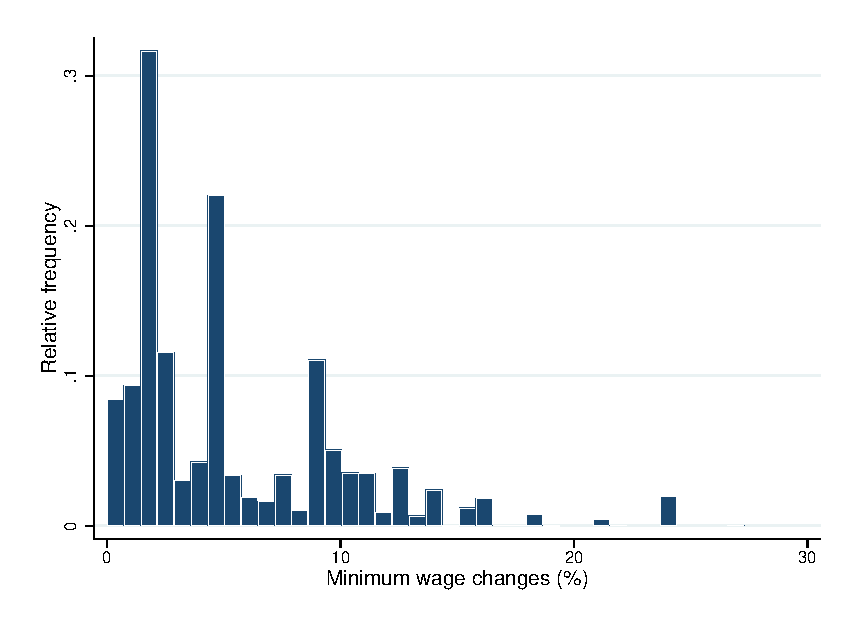
\includegraphics[width = \textwidth]
            {estimation_samples/output/pct_ch_mw_dist}
    \end{subfigure}\\
    \begin{subfigure}{.7\textwidth}
        \caption{Timing}
        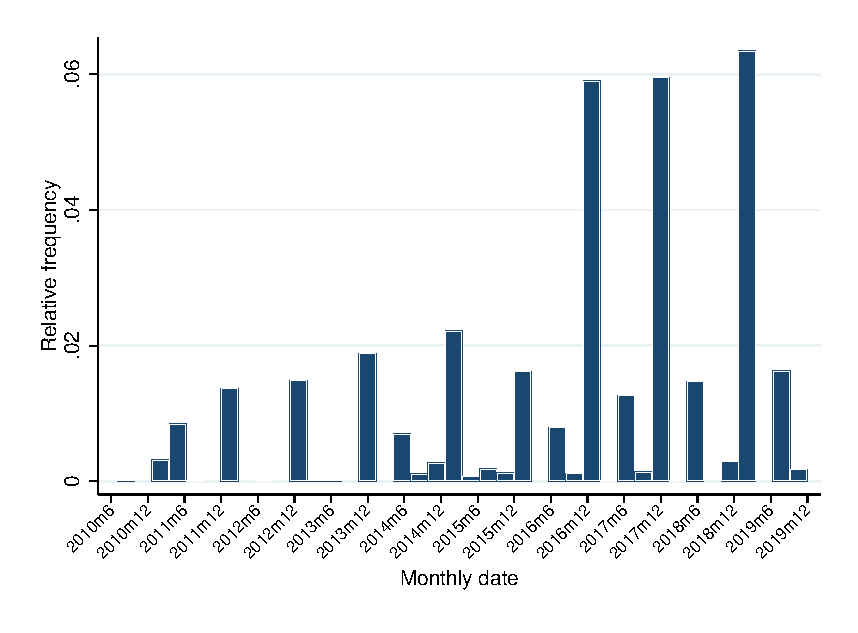
\includegraphics[width = \textwidth]
            {estimation_samples/output/pct_ch_mw_date_dist}
    \end{subfigure}

    \begin{minipage}{.95\textwidth} \footnotesize
        \vspace{3mm}
        Notes:
        Data are from the minimum wage panel described in 
        Section \ref{sec:mw_construction}.
        The histograms show the distribution of positive MW changes in the full 
        sample of ZIP codes available in the Zillow data.
        Panel (a) reports the intensity of the changes in percentage terms.
        Panel (b) plots the distribution of such changes over time.
    \end{minipage}
\end{figure}

\clearpage
\begin{figure}[h!]
    \centering
    \caption{Changes in minimum wage measures in the Chicago-Naperville-Elgin CBSA, July 2019}
    \label{fig:map_mw_chicago_jul2019}

    \begin{subfigure}{0.5\textwidth}
        \centering
        \caption{Residence MW}
        \includegraphics[width = 1\textwidth]
            {maps_events/output/chicago_2019-6_statutory_mw}
    \end{subfigure}%
    \begin{subfigure}{0.5\textwidth}
        \centering
        \caption{Workplace MW}
        \includegraphics[width = 1\textwidth]
            {maps_events/output/chicago2019-6_wkp_mw}
    \end{subfigure}

    \begin{minipage}{.95\textwidth} \footnotesize
        \vspace{3mm}
        Notes: 
        Data are from the MW panel described in
        Section \ref{sec:data_mw_panel} and from LODES.
        The figure shows the change in 
        the residence MW (panel a) and workplace MW (panel b) 
        in July 2019 in the metropolitan area of Chicago.
        The residence MW is defined as the log of the statutory MW of the given
        ZIP code.
        The workplace MW is defined as the weighted average of the log of the
        statutory MW levels in workplace locations of a ZIP code's residents,
        where weights are given by commuting shares.
    \end{minipage}
\end{figure}

\clearpage

\begin{figure}[h!]
    \centering
    \caption{Estimates of the effect of the MW on rents, baseline sample 
             including leads and lags}
    \label{fig:dynamic_baseline}

    \begin{subfigure}{.5\textwidth}
        \caption{Leads and lags of the workplace MW}
        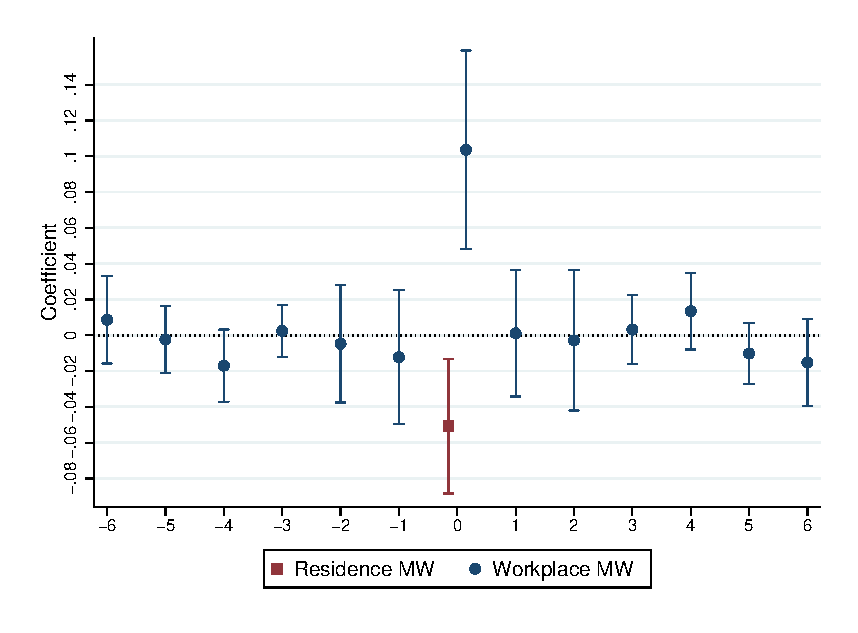
\includegraphics[width = 1\textwidth]
            {fd_baseline/output/fd_both_mw_wkp_only_dynamic}
    \end{subfigure}\\
    \begin{subfigure}{.5\textwidth}
        \caption{Leads and lags of the residence MW}
        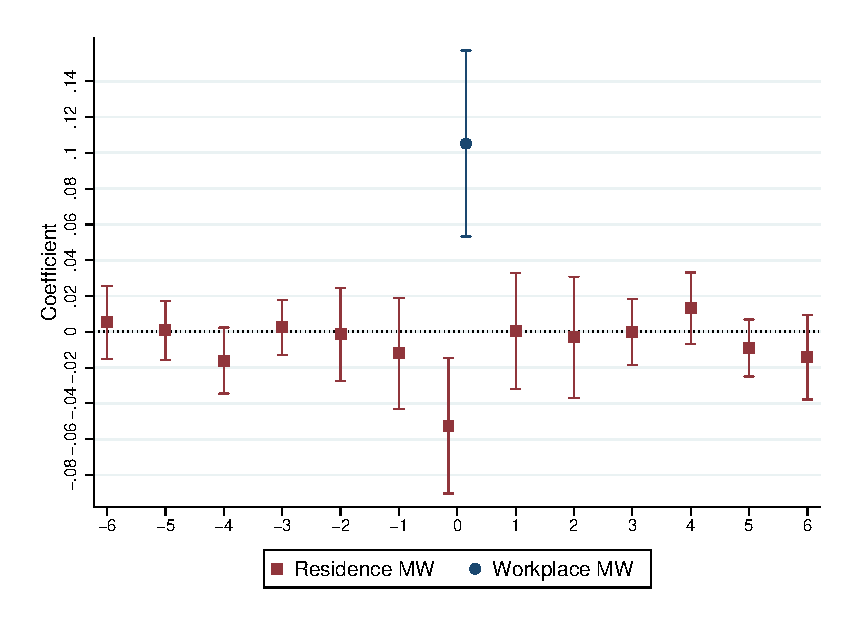
\includegraphics[width = 1\textwidth]
            {fd_baseline/output/fd_both_mw_res_only_dynamic}
    \end{subfigure}%
    \begin{subfigure}{.5\textwidth}
        \caption{Leads and lags of both wkp.\ and res.\ MW}
        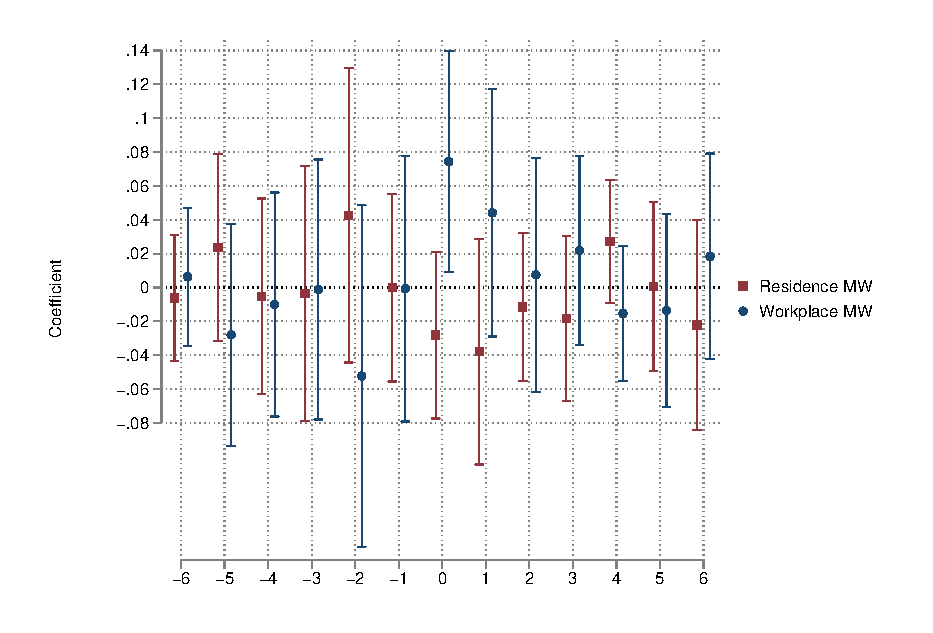
\includegraphics[width = 1\textwidth]
            {fd_baseline/output/fd_both_dynamic}
    \end{subfigure}

    \begin{minipage}{.95\textwidth} \footnotesize
        \vspace{3mm}
        Notes:
        Data are from the baseline estimation sample described in Section 
        \ref{sec:data_final_panel}.
        All panels plot coefficients from regressions of the log of rents per
        square foot on the residence and workplace MW measures, varying the 
        number of leads and lags of each MW variable included.
        Panel (a) includes six leads and lags of the workplace MW measure.
        Panel (b) includes six leads and lags of the residence MW measure.
        Panel (c) includes six leads and lags of both MW measures.
        All regressions are estimated in first differences and include 
        time-period fixed effects and economic controls that vary at the 
        county and month levels.
        The measure of rents per square foot correspond to the Single Family, 
        Condominium and Cooperative houses from Zillow.
        The residence MW is defined as the log statutory MW in the same ZIP code.
        The workplace MW is defined as the statutory MW where the average 
        resident of the ZIP code works, constructed using LODES 
        origin-destination data.
        Economic controls from the QCEW include the change of the following 
        variables: the log of the average wage, the log of employment, and the 
        log of the establishment count for the sectors ``Information,'' 
        ``Financial activities,'' and ``Professional and business services.''
        95\% pointwise confidence intervals are obtained from standard errors 
        clustered at the state level.
    \end{minipage}
\end{figure}

\clearpage
\begin{figure}[h!]
    \centering
    \caption{Distributions of estimated landlord shares and counterfactual 
                changes in rents and total wages, urban ZIP codes}
    \label{fig:cf_hist_rents_wages_shares}

    \begin{subfigure}{0.65\textwidth}
        \caption*{Landlord share}
        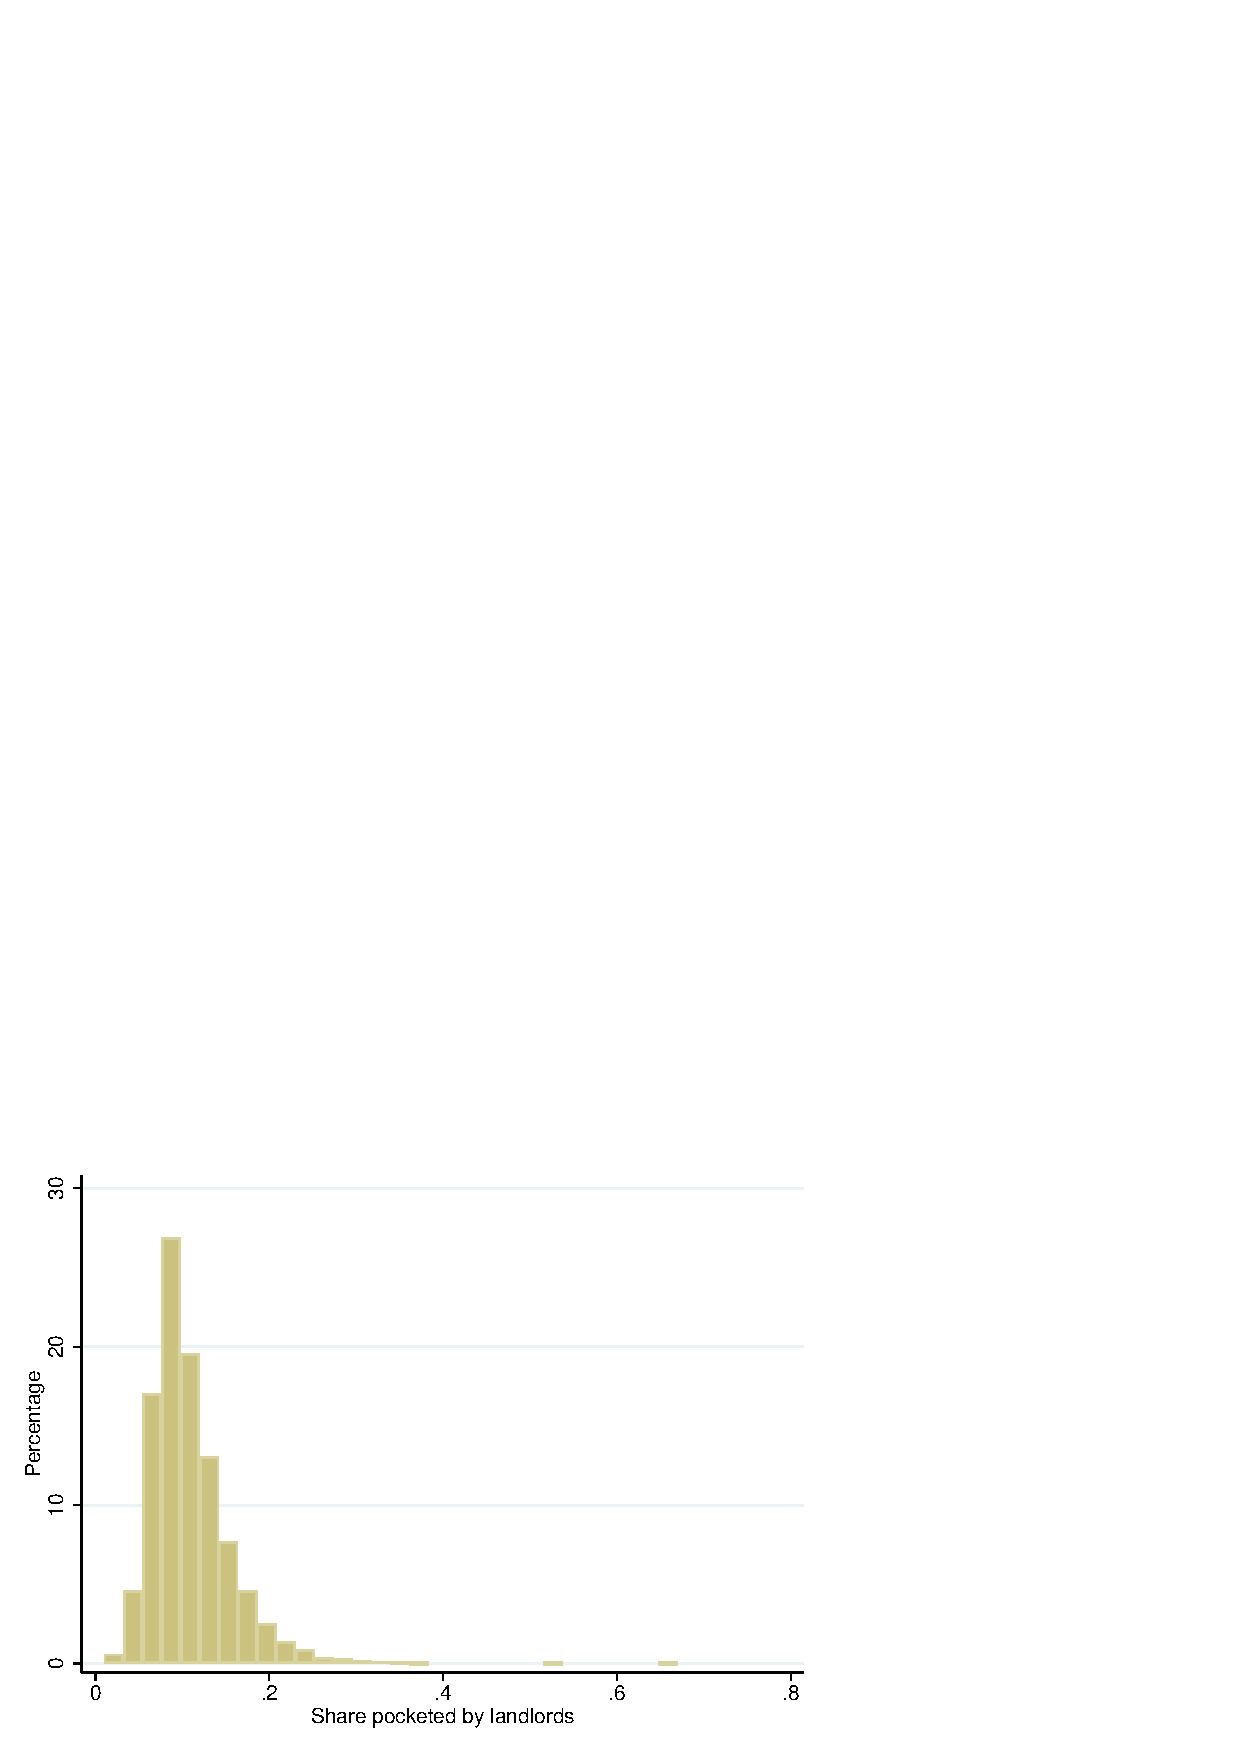
\includegraphics[width = 1\textwidth]{counterfactuals/output/hist_rho.png}
    \end{subfigure}\\
    \begin{subfigure}{0.5\textwidth}
        \includegraphics[width = .95\textwidth]{counterfactuals/output/hist_perc_incr_rent.png}
        \caption*{Log(rents)}
    \end{subfigure}%
    \begin{subfigure}{0.5\textwidth}
        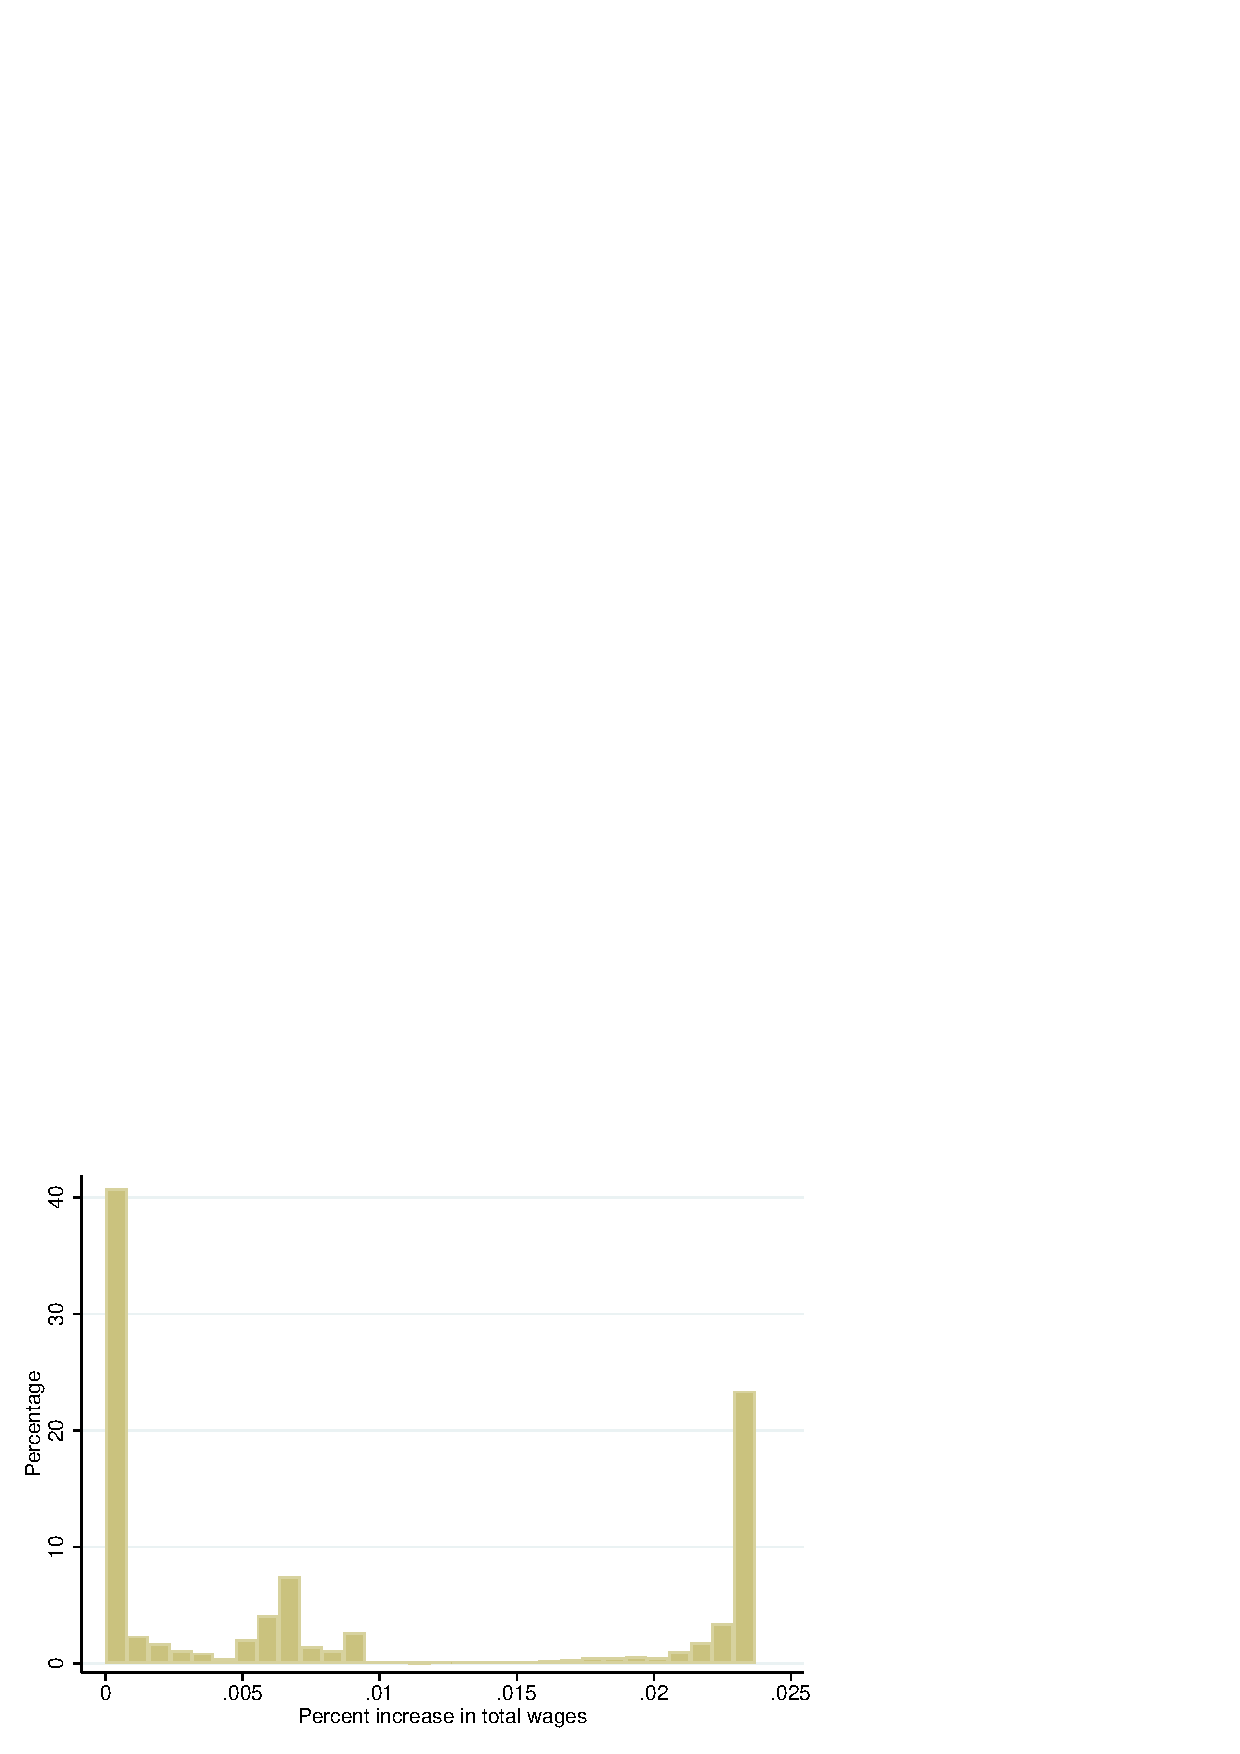
\includegraphics[width = .95\textwidth]{counterfactuals/output/hist_perc_incr_wagebill.png}
        \caption*{Log(total wages)}
    \end{subfigure}

    \begin{minipage}{.95\textwidth} \footnotesize
        \vspace{3mm}
        Notes: 
        Data are from the LODES and the minimum wage panel described in Section 
        \ref{sec:mw_construction}.
        The figures show the distribution of estimated landlord shares in 
        panel (a), estimated changes in log rents in panel (b) and 
        estimated changes in log total wages in panel (c),
        generated by a counterfactual increase to \$9 in the federal MW in 
        January 2020, holding constant other MW policies in their December 2019 
        levels.
        The unit of observation is the urban ZIP code, where we define a ZIP code 
        as urban if at least 80\% of its population is classified as urban by
        the 2010 Census.
        The landlord share is defined as the ratio between the increase in rents
        and the increase in total wages multipled by the share of housing 
        expenditure in the ZIP code, assumed to be 0.35 for all ZIP codes.
    \end{minipage}
\end{figure}

\clearpage
\begin{figure}[h!]
    \centering
    \caption{Estimated landlord shares and counterfactual increases in log rents
            and log total wages, ZIP codes in the Chicago-Naperville-Elgin CBSA}
    \label{fig:map_chicago_cf_rents_wages_shares}

    \begin{subfigure}{.5\textwidth}
        \caption*{Landlord share}
        \includegraphics[width = 1\textwidth]
            {counterfactuals/output/chicago_rho.png}
    \end{subfigure}\\
    \begin{subfigure}{.35\textwidth}
        \caption*{Changes in log rents}
        \includegraphics[width = 1\textwidth]
            {counterfactuals/output/chicago_d_ln_rents.png}
    \end{subfigure}%
    \begin{subfigure}{.35\textwidth}
        \caption*{Changes in log total wages}
        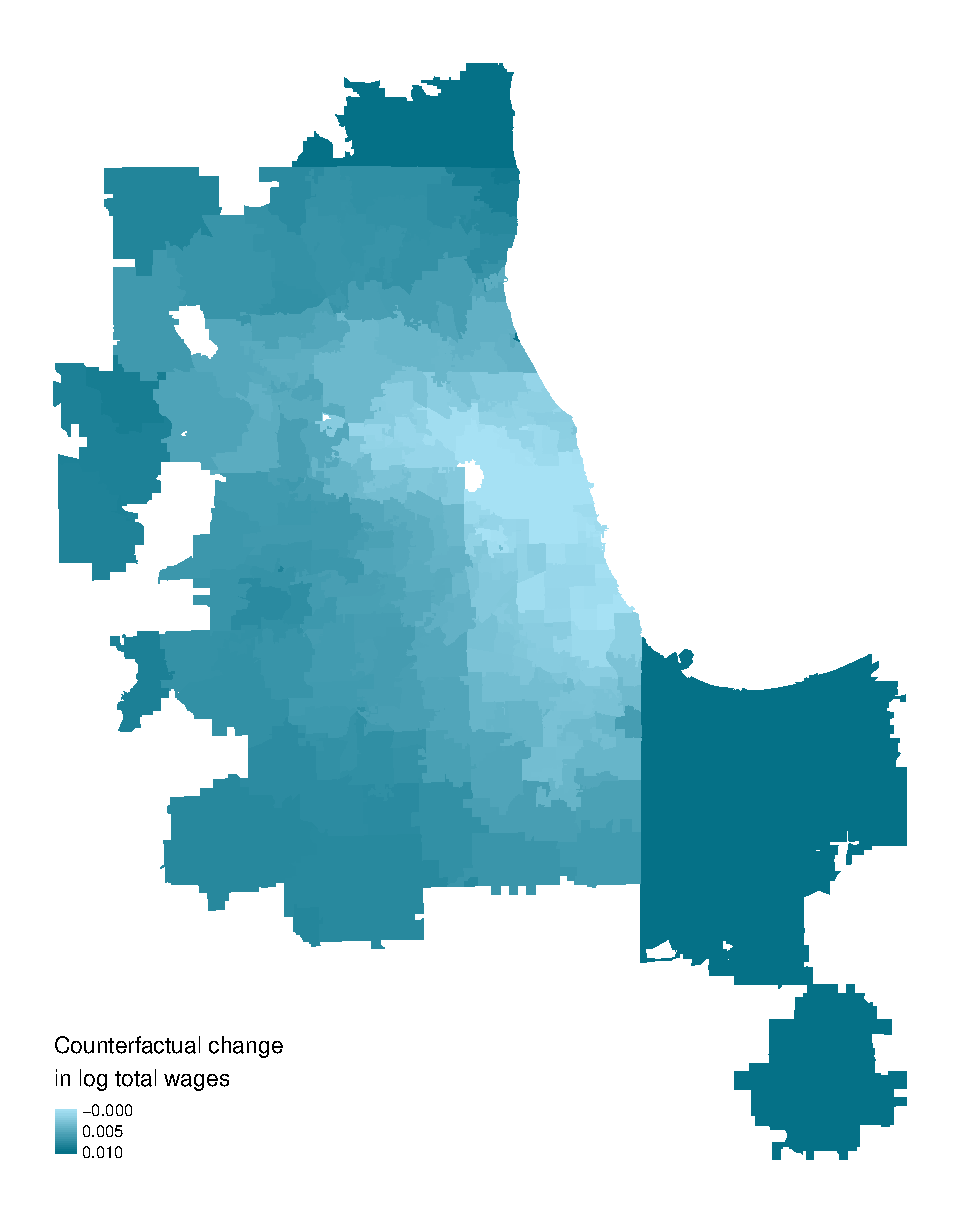
\includegraphics[width = 1\textwidth]
            {counterfactuals/output/chicago_d_ln_wagebill.png}
    \end{subfigure}

    \begin{minipage}{.95\textwidth} \footnotesize
        \vspace{3mm}
        Notes: 
        Data are from LODES and the minimum wage panel described in Section 
        \ref{sec:mw_construction}.
        The top figures maps the distribution of estimated landlord shares, 
        the bottom left figure maps estimated changes in log rents, and 
        the bottom right figure maps estimated changes in log total wages,
        for ZIP codes in the Chicago-Naperville-Elgin CBSA.
        The computations are based on a counterfactual increase to \$9 in the 
        federal MW in January 2020, holding constant other MW policies in their 
        December 2019 levels.
        The landlord share is defined as the ratio between the percent increase 
        in rents and the percent increase in total wages multipled by the share 
        of housing expenditure in the ZIP code.
        To estimate it we follow the procedure described in Section 
        \ref{sec:counterfactual}, assuming the following parameter values: 
        $\beta = 0.0546$, $\gamma = -0.0207$, $\varepsilon = 0.1083$, and 
        $s = 0.35$.
    \end{minipage}
\end{figure}

\clearpage
\begin{figure}[h!]
    \centering
    \caption{Share pocketed by landlords by intensity of treatment, 
             urban ZIP codes under federal MW increase to \$9}
    \label{fig:rho_by_decile_MW_gap}

	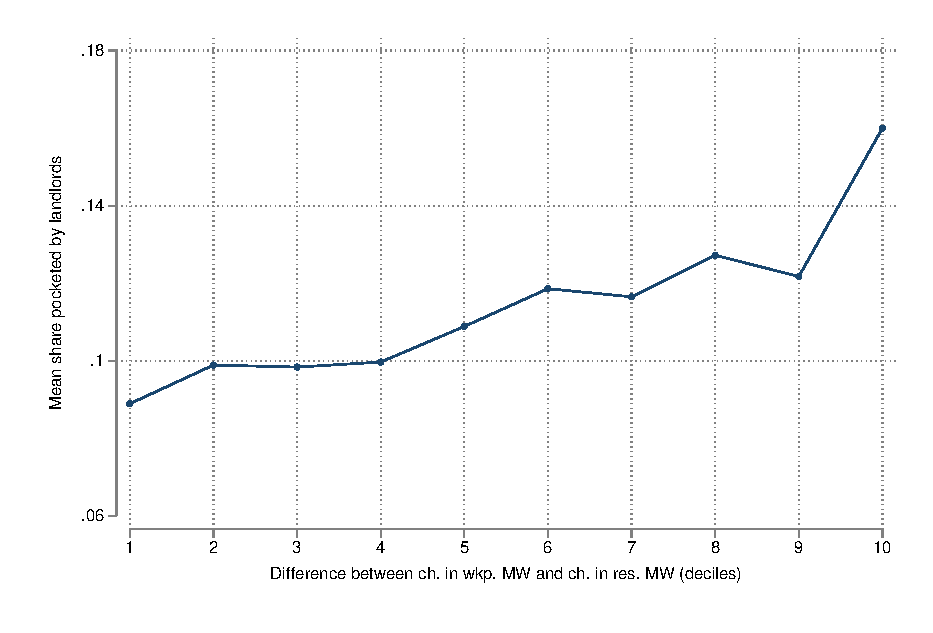
\includegraphics[width = 0.75\textwidth]{counterfactuals/output/deciles_diff_fed_9usd}

    \begin{minipage}{.95\textwidth} \footnotesize
        \vspace{3mm}
        Notes:
        Data are from the MW panel described in Section \ref{sec:data_mw_panel} 
        and from LODES.
        The figure shows the average estimate of the shares of additional
        income pocketed by landlords $\rho_i$ for each decile of the 
        difference $\Delta \mw_i^{\wkp} - \Delta \mw_i^{\res}$.
        Estimates for lower deciles correspond to ZIP codes where the increase 
        in residence MW was relatively large.
        The unit of observation is the urban ZIP code, where we define a ZIP code 
        as urban if it belongs to a CBSA with at least 80\% of its population 
        classified as urban by the 2010 Census.
        The share pocketed is defined as the ratio between the percent increase 
        in rents and the percent increase in total wages multiplied by the share 
        of housing expenditure in the ZIP code.
        To estimate it we follow the procedure described in Section 
        \ref{sec:counterfactual}, assuming the following parameter values: 
        $\beta = \betaCf$, $\gamma = \gammaCf$, and $\varepsilon = \epsilonCf$.
        The figure excludes ZIP codes located in the $\cbsaLowIncFedNine$ CBAs for which the average
        estimated change in log total wages was below 0.1.
    \end{minipage}
\end{figure}


\clearpage

\begin{landscape}
\begin{table}[hbt!] \centering
    \caption{Descriptive statistics of different samples of ZIP codes}
    \label{tab:stats_zip_samples}
    \begin{tabular}{@{}lcccc@{}}
        \toprule
                                                         & \multicolumn{1}{p{2cm}}{\centering All\\ZIP codes}
                                                         & \multicolumn{1}{p{2cm}}{\centering Urban\\ZIP codes}
                                                         & \multicolumn{1}{p{2cm}}{\centering Zillow\\sample}
                                                         & \multicolumn{1}{p{2cm}}{\centering Baseline\\sample}  \\ \midrule
        (a) Mean population, 2010                        & 9,681.7 & 19,488.0 & 33,687.9  & 38,052.9     \\
        (b) Mean number of households, 2010              & 4,128.6 & 8,151.1 & 14,301.7  & 16,080.8     \\
        (c) Share urban population, 2010                 & 0.391    & 0.862   & 0.960   & 0.972          \\
        (d) Share renter households, 2010                & 0.224    & 0.306   & 0.340   & 0.333          \\
        (e) Share black population, 2010                 & 0.075    & 0.114   & 0.153   & 0.161          \\
        (f) Share white population, 2010                 & 0.834    & 0.760   & 0.679   & 0.667          \\
        (g) Share male population, 2010                  & 0.502    & 0.494   & 0.489   & 0.488          \\
        (h) Share households with wage income, 2010      & 0.822    & 0.834   & 0.833   & 0.840          \\
        (i) Share households with business income, 2010  & 0.159    & 0.152   & 0.166   & 0.170          \\
        (j) Mean AGI per household (\$), 2010            & 53,233.4 & 61,238.3 & 70,264.4 & 71,150.6     \\
        (k) Mean wage income per household (\$), 2010    & 36,237.8 & 42,011.6 & 47,469.6 & 49,287.6     \\
        (l) Mean 40th perc.\ 2BR apt.\ rent (\$), 2012   & 887.23   & 957.03  & 1,039.50  & 1,076.72     \\
        (m) Min statutory MW (\$), Feb.\ 2010            & 7.25   & 7.25  & 7.25  & 7.25                \\
        (n) Mean statutory MW (\$), Feb.\ 2010           & 7.41   & 7.45  & 7.48  & 7.43                \\
        (o) Max statutory MW (\$), Feb.\ 2010            & 10.10   & 10.10  & 10.10  & 9.79              \\
        (p) Min statutory MW (\$), Dec.\ 2019            & 7.25   & 7.25  & 7.25  & 7.25                 \\
        (q) Mean statutory MW (\$), Dec.\ 2019           & 8.83   & 9.23  & 9.38  & 9.21                 \\
        (r) Max statutory MW (\$), Dec.\ 2019            & 16.00   & 16.00  & 16.00  & 16.00              \\
        (s) Number of ZIP codes                          & 31,826  & 13,884 & 3,316 & 1,345               \\ \bottomrule
    \end{tabular}

    \begin{minipage}{.95\linewidth} \footnotesize
        \vspace{2mm}
        Notes: The table shows characteristics of different samples of ZIP codes.
        The first column uses all valid USPS ZIP codes.
        The second restricts to urban ZIP codes, where we define a ZIP code as 
        rural if it has at least 60\% of its population was classified as rural 
        by the 2010 US Census \parencite{CensusDecennial}.
        The third and fourth columns use the ZIP codes with valid SFCC rents 
        data, and the ones used in the baseline estimation, as described in
        Section \ref{sec:data}.
        Each row shows a given characteristic obtained from different a data 
        source.
        Rows (a)--(g) are constructed from the 2010 US Census \parencite{CensusDecennial}.
        Rows (h)--(k) are obtained from 2011 IRS ZIP code-level statiscs 
        \parencite{IRS}. AGI is an acronym for Average Gross Income.
        Row (l) is obtained from SAFMR \parencite{hudSAFMR}.
        Rows (m)--(s) are computed using the panel of minimum wage levels 
        described in Section \ref{sec:mw_construction}.
    \end{minipage}
\end{table}
\end{landscape}

\clearpage
\begin{table}
    \caption{Static model}
    \label{tab:static}
    \scalebox{0.8}{
    \begin{tabular}{l*{4}{c}}
        \toprule
        & \multicolumn{1}{c}{Change workplace MW}
            & \multicolumn{3}{c}{Change log rents}                            \\ \cmidrule(lr){2-2}\cmidrule(lr){3-5}
                                           & (1)   & (2)   & (3)   & (4)      \\ \midrule
        Change residence minimum wage      &  #4#  &  #4#  &       &  #4#     \\
                                           & (#4#) & (#4#) &       & (#4#)    \\
        Change workplace minimum wage      &       &       &  #4#  & #4#      \\
                                           &       &       & (#4#) & (#4#)    \\ \midrule
        Sum of coefficients                &       &       &       &  #4#     \\
                                           &       &       &       & (#4#)    \\
                                           &       &       &       &          \\ \midrule
        County-quarter economic controls   &  Yes  & Yes   & Yes   & Yes      \\
        P-value equality                   &       &       &       & #4#      \\
        R-squared                          &  #4#  &  #4#  &  #4#  & #4#      \\
        Observations                       & #0,#  & #0,#  & #0,#  & #0,#     \\\bottomrule
    \end{tabular}}

    \begin{minipage}{.95\textwidth} \footnotesize
        \vspace{2mm}
        Notes: 
    \end{minipage}
\end{table}

\clearpage
\begin{table}[hbt!]
    \caption{Estimates of the effect of the MW on rents, different samples}
    \label{tab:static_sample}

    \begin{tabular}{@{}lcccccc@{}}
        \toprule
                                             & \multicolumn{4}{c}{Change in log rents $\Delta r_{it}$}                   \\ \cmidrule(l){2-5} 
                                             & \shortstack{Baseline\\(1)}       & \shortstack{Unbalanced\\(2)}     
                                             & \shortstack{Fully-balanced\\(3)} & \shortstack{Baseline\\Reweighted (4)}  \\ \midrule
        Change in residence MW 
                  $\Delta\mw_{it}^{\res}$    & -0.0204      & -0.0240        & -0.0194       & 0.1918               \\
                                             & (0.0169)    & (0.0200)      & (0.0198)     & (0.1919)              \\
        Change in workplace MW 
                   $\Delta\mw_{it}^{\wkp}$   & 0.0545      & 0.0461        & 0.0678       & -0.1439               \\
                                             & (0.0283)    & (0.0305)      & (0.0308)     & (0.1947)              \\ \midrule
        P-value equality                     & 0.0965      & 0.1586        & 0.0826       & 0.3895               \\
        R-squared                            & 0.0209      & 0.0160        & 0.0216       & 0.0319               \\
        Observations                         & 131,383     & 193,292       & 78,912      & 125,502             \\ \bottomrule
    \end{tabular}

    \begin{minipage}{.95\textwidth} \footnotesize
        \vspace{2mm}
        Notes:
        Data are from Zillow \parencite{ZillowData}, 
        the statutory MW panel described in Section \ref{sec:mw_construction}, 
        LODES origin-destination statistics \parencite{CensusLODES},
        and the QCEW \parencite{QCEW}.
        Every column show the results of regressions of the log of 
        median rents per square foot on our MW-based measures.
        All regressions are estimated in first differences and include 
        time-period fixed effects and economic controls that vary at the 
        county and month levels.
        The measure of rents per square foot correspond to the Single Family, 
        Condominium and Cooperative houses from Zillow.
        Column (1) uses our baseline sample defined in Section 
        \ref{sec:data_final_panel}.
        Column (2) uses the unbalanced sample of all ZIP codes with Zillow rents 
        data at any point in time, and controls for year of entry to the panel
        $\times$ year-month fixed effects.
        Column (3) uses a fully-balanced panel that, starting from the baseline
        panel, drops all data before July 2015.
        Column (4) uses the baseline panel and reweights observations so that 
        the sample of ZIP codes in the data has the same averages that the set 
        of urban ZIP codes in the following variables:
        share of white population (census 2010), 
        share of African-American population (census 2010),
        share of renter-occupied households (census 2010),
        median household income (ACS 2011).
        The re-weigthing procedure follows \textcite{Hainmueller2012}.
    \end{minipage}
\end{table}

\clearpage
\begin{table}[hbt!] \centering
    \caption{Estimates of the effect of the MW on rents by share of MW workers, baseline sample}
    \label{tab:heterogeneity}
    \begin{tabular}{@{}lccc@{}}
        \toprule
            & \multicolumn{3}{c}{Change log rents}                                                  \\ \cmidrule(l){2-4} 
            & \shortstack{Baseline\\(1)} 
            & \shortstack{MW shares\\(2)}                                             
            & \shortstack{Public housing\\(3)}                                                      \\ \midrule
        Change residence minimum wage                                     &  -0.0207   &  -0.0136  &  -0.0002   \\
                                                                          & (0.0171)  & (0.0175) & (0.0250)  \\
        Change residence minimum wage $\times$ High share of MW workers   &        &  -0.0284  &        \\
                                                                          &        & (0.0175) &        \\
        Change residence minimum wage $\times$ Public housing             &        &       &  -0.0618   \\
                                                                          &        &       & (0.0388)  \\
        Change workplace minimum wage                                     &  0.0546   &  0.0491  &  0.0331   \\
                                                                          & (0.0281)  & (0.0274) & (0.0329)  \\
        Change workplace minimum wage $\times$ High share of MW residents &        &  0.0583  &        \\
                                                                          &        & (0.0286) &        \\
        Change workplace minimum wage $\times$ Public housing             &        &       &  0.0976   \\
                                                                          &        &       & (0.0445)  \\
        County-quarter economic controls                                  &  Yes   &  Yes  &   Yes  \\
        R-squared                                                         &  0.0209   &  0.0239  &   0.0222  \\
        Observations                                                      &  131,383  &  131,380 &   131,383 \\ \bottomrule
    \end{tabular}

    \begin{minipage}{.95\textwidth} \footnotesize
        \vspace{2mm}
        \textit{Notes}: 
        Rents and MW data are from the baseline estimation sample described in Section 
        \ref{sec:data_final_panel}.
        Public housing data are from \ref{hudHousing}.
        In all columns we report the results of regressions of the log of median rents 
        per square foot on our MW-based measures.
        Column (1) reproduces estimates our baseline results from Table \ref{tab:static}.
        Column (2) presents estimates of our baseline model in which the residence MW 
        measure is interacted with an indicator that proxies for having a high share 
        of MW workers (``High share of MW workers'') and the workplace MW measure is 
        fully interacted with an indicator that proxies for having a high share of MW 
        residents (``High share of MW residents'').
        We define the indicators as follows.
        First, using LODES data we create indicator for being above the within-state 
        median across basline ZIP codes in the following variables: (i) share of workers 
        with less than a high school diploma, (ii) share of workers who earn earn less 
        than \$1251, (iii) share of residents with less than a high school diploma, (iv) 
        share of residents who earn earn less than \$1251.
        Second, we define the indicator ``High share of MW workers'' as 1 if the ZIP
        code is above median of both (i) and (ii), and the indicator ``High share of MW 
        residents'' if the ZIP code is above median of both (iii) and (iv).
        Column (3) presents estimates of our baseline model in which the residence and 
        the workplace MW measures are interacted with an indicator that equals 1 if 
        the ZIP code has any public housing units.
        Both columns (2) and (3) fully interact the MW measures and the fixed effects
        with the indicator variables.
        The time fixed effects are interacted with the indicators and the economic controls 
        are not.
    \end{minipage}
\end{table}

\clearpage
\begin{landscape}
\begin{table}[ht!]
    \centering
    \caption{Estimates of the effect of the MW on rents, robustness}
    \label{tab:robustness}
        
    \begin{tabular}{@{}lccccc@{}}
        \toprule
                                                         & \shortstack{Change wkp.\\MW $\Delta\mw_{it}^{\wkp}$} 
                                                         & \multicolumn{3}{c}{\shortstack{Change log rents\\$\Delta r_{it}$}} 
                                                         &                                                                           \\ \cmidrule(lr){2-2}\cmidrule(lr){3-5}
                                                             & \multicolumn{1}{c}{\shortstack{Change res.\\MW $\Delta\mw_{it}^{\res}$}}
                                                             & \multicolumn{1}{c}{\shortstack{Change res.\\MW $\Delta\mw_{it}^{\res}$}}
                                                             & \multicolumn{1}{c}{\shortstack{Change wkp.\\MW $\Delta\mw_{it}^{\wkp}$}} 
                                                             & \shortstack{Sum of\\coefficients}
                                                             & N                                                                      \\ \midrule
        $\quad$(a) Baseline                                  &  #4#  &  #4#  &  #4#  &  #4#  & #0,# \\
                                                             & (#4#) & (#4#) & (#4#) & (#4#) &      \\
        \textit{Panel A: Vary specification}                 &       &       &       &       &      \\
        $\quad$(b) No controls                               &  #4#  &  #4#  &  #4#  &  #4#  & #0,# \\
                                                             & (#4#) & (#4#) & (#4#) & (#4#) &      \\
        $\quad$(c) County $\times$ time FE                   &  #4#  &  #4#  &  #4#  &  #4#  & #0,# \\
                                                             & (#4#) & (#4#) & (#4#) & (#4#) &      \\
        $\quad$(d) CBSA $\times$ time FE                     &  #4#  &  #4#  &  #4#  &  #4#  & #0,# \\
                                                             & (#4#) & (#4#) & (#4#) & (#4#) &      \\
        $\quad$(e) State $\times$ time FE                    &  #4#  &  #4#  &  #4#  &  #4#  & #0,# \\
                                                             & (#4#) & (#4#) & (#4#) & (#4#) &      \\
        $\quad$(f) ZIP code-specific linear trend            &  #4#  &  #4#  &  #4#  &  #4#  & #0,# \\
                                                             & (#4#) & (#4#) & (#4#) & (#4#) &      \\
        \textit{Panel B: Vary workplace MW measure}          &       &       &       &       &      \\
        $\quad$(g) 2014 commuting shares                     &  #4#  &  #4#  &  #4#  &  #4#  & #0,# \\
                                                             & (#4#) & (#4#) & (#4#) & (#4#) &      \\
        $\quad$(h) 2018 commuting shares                     &  #4#  &  #4#  &  #4#  &  #4#  & #0,# \\
                                                             & (#4#) & (#4#) & (#4#) & (#4#) &      \\
        $\quad$(i) Time-varying commuting shares             &  #4#  &  #4#  &  #4#  &  #4#  & #0,# \\
                                                             & (#4#) & (#4#) & (#4#) & (#4#) &      \\
        $\quad$(j) 2017 commuting shares, low-income workers &  #4#  &  #4#  &  #4#  &  #4#  & #0,# \\
                                                             & (#4#) & (#4#) & (#4#) & (#4#) &      \\
        $\quad$(k) 2017 commuting shares, young workers      &  #4#  &  #4#  &  #4#  &  #4#  & #0,# \\
                                                             & (#4#) & (#4#) & (#4#) & (#4#) &      \\ \bottomrule
    \end{tabular}

    \begin{minipage}{.95\linewidth} \footnotesize
        \vspace{2mm}
        Notes: 
        Data are from the baseline estimation sample described in Section 
        \ref{sec:data_final_panel}.
        Each row of the table shows two estimations on the same sample of ZIP 
        codes and months.
        The first column shows the results of a regression of the change in the 
        workplace MW measure on the change in the residence MW measure.
        The second through fourth columns show the results of a regression of 
        the change in log rents on the change in the residence MW and the 
        workplace MW, with the fifth column showing the sum of the coefficients 
        on the MW measures.
        The rents variable corresponds to the median rent per square foot in
        the Zillow data.
        Row (a) repeats the results of Table \ref{tab:static}, including fixed
        effects for each year month and economic controls at the 
        county $\times$ quarter level.
        Specifications in Panel A vary the set of controls included in the 
        regression relative to row (a).
        Row (f) includes ZIP code fixed effects in the first-differenced model,
        which in the level model can be interpreted as a ZIP-code specific 
        linear trend.
        Specifications in Panel B vary the commuting shares used to construct 
        the workplace MW measure relative to row (a).
        Standard errors in parenthesis are clustered at the state level.
    \end{minipage}
\end{table}
\end{landscape}

\clearpage
\begin{table}[hbt!]
    \centering
    \caption{Effect of an increase in federal MW to \$9 in January 2020, urban ZIP codes}
    \label{tab:counterfactuals_fed_9usd}

    \begin{tabular}{@{}lccccc@{}}
        \toprule
                            & 
                            & \multicolumn{2}{c}{Average change in...} 
                            & \multirow{2}{*}{\thead{Avg.\ share of\\housing exp.}}   
                            &  \multirow{2}{*}{\thead{Avg.\ share\\pocketed}} \\ \cmidrule(lr){3-4}
                            & N & Res.\ MW & Wkp.\ MW \\ \midrule
        Effect in ZIP codes with...          &      &       &       &     &      \\
        $\quad$previous MW $\leq\$9\quad$    & #0,# &  #3# & #3#  & #3# &  #3#   \\
        $\quad$previous MW $>\$9\quad$       & #0,# &  #3# & #3#  & #3# & #3#    \\ \bottomrule
    \end{tabular}
    
    \begin{minipage}{.95\textwidth} \footnotesize
        \vspace{2mm}
        Notes: 
        Data are from LODES and the minimum wage panel described in Section 
        \ref{sec:mw_construction}.
        The table shows averages of the estimated ZIP-code specific shares of the 
        additional income pocketed by landlords (``Avg.\ share pocketed''), 
        defined as the ratio of the increase in income to the increase in rents.
        We also report the average share of ZIP-code specific housing expenditure
        (``Avg.\ share of housing exp.''), defined as explained in XXXX.
        Increases in income and rents are simulated following the procedure 
        described in Section \ref{sec:counterfactual}, 
        where we assume an increase in the federal MW to \$9.
        We assume the following parameter values: 
        $\beta = \betaCounterfactual$, $\gamma = \gammaCounterfactual$, and $\varepsilon = \epsilonCounterfactual$.
        We carry out our computations only for urban ZIP codes, defined as 
        those that belong to a CBSA with at least 80\% of urban population
        according to the 2010 census.
        The table excludes ZIP codes located in the 60 CBAs for which the average
        estimated change in log total wages was below 0.1\%.
    \end{minipage}
\end{table}


%%%%%%%%%%%%%%%%%%%%%%%%%%%%%%%%%%%%%%%%%%%%%%%%%%%%%%%%%%%%%%%%%%%%%%%%%%%%%%%%
%%%%                             APPENDIX                                   %%%%
%%%%%%%%%%%%%%%%%%%%%%%%%%%%%%%%%%%%%%%%%%%%%%%%%%%%%%%%%%%%%%%%%%%%%%%%%%%%%%%%

\clearpage

\section*{\centering{Appendix}}
\vspace{5mm}

\appendix

\renewcommand\thetable{\arabic{table}} 
\renewcommand\thefigure{\arabic{figure}}
\renewcommand{\tablename}{Appendix Table}
\renewcommand{\figurename}{Appendix Figure}
\setcounter{table}{0}
\setcounter{figure}{0}

%%%%%%%%%%%%%%%%%%%%%%%%%%%%%%%%%%%%%%%%%%%%%%%%%%%%%%%%%%%%%%%%%%%%%%%%%%%%%%%%%
%%%%%                           ONLINE APPENDIX                              %%%%
%%%%%%%%%%%%%%%%%%%%%%%%%%%%%%%%%%%%%%%%%%%%%%%%%%%%%%%%%%%%%%%%%%%%%%%%%%%%%%%%%

%%%%%%%%%%%%%%%%%%%%%%%%%%%%%%%%%%%%%%%%%%%%%%%%%%%%%%%%%%%%%%%%%%%%%%%%%%%%%%%%%
\section{Appendix Tables}

\begin{table}[h!]
	\caption{Descriptive statistics of estimating panel: more variables}
	\label{tab:estimating_panel_stats_long}
	\centering
	
% Table created by stargazer v.5.2.2 by Marek Hlavac, Harvard University. E-mail: hlavac at fas.harvard.edu
% Date and time: Mon, Nov 30, 2020 - 11:59:19 AM
\begin{tabular}{@{\extracolsep{5pt}}lccccc} 
\\[-1.8ex]\hline 
\hline \\[-1.8ex] 
Statistic & \multicolumn{1}{c}{N} & \multicolumn{1}{c}{Mean} & \multicolumn{1}{c}{St. Dev.} & \multicolumn{1}{c}{Min} & \multicolumn{1}{c}{Max} \\ 
\hline \\[-1.8ex] 
Statutory MW & 156,600 & 8.08 & 1.21 & 7 & 16 \\ 
Experienced MW (total jobs) & 156,600 & 8.06 & 1.20 & 6.29 & 14.98 \\ 
Experienced MW (low inc.) & 156,600 & 8.06 & 1.20 & 5.81 & 15.02 \\ 
Experienced MW (young) & 156,600 & 8.06 & 1.20 & 6.19 & 15.07 \\ 
Median rent psqft. 2BR & 24,789 & 1.96 & 0.97 & 0.53 & 6.51 \\ 
Median rent psqft. MFR5plus & 37,588 & 1.96 & 1.05 & 0.55 & 6.69 \\ 
Median rent psqft.SFCC & 113,375 & 1.27 & 0.83 & 0.47 & 7.25 \\ 
Median rent SFCC & 125,644 & 1,651.10 & 702.99 & 595.00 & 6,595.00 \\ 
Avg. wage Fin. activities & 152,334 & 1,561.78 & 965.27 & 0.00 & 9,557.00 \\ 
Employment Fin. activities & 152,334 & 59,554.22 & 75,796.09 & 0.00 & 397,839.00 \\ 
Estab. count Fin. activities & 152,334 & 5,103.83 & 5,200.06 & 31.00 & 30,405.00 \\ 
Avg. wage Prof. and bus. serv. & 152,334 & 1,252.94 & 434.75 & 226.00 & 4,727.00 \\ 
Employment Prof. and bus. serv. & 152,334 & 134,280.40 & 143,863.40 & 329.00 & 640,795.00 \\ 
Estab. count Prof. and bus. serv. & 152,334 & 9,999.11 & 9,479.67 & 60.00 & 56,758.00 \\ 
Avg. wage Information & 152,334 & 1,505.07 & 619.82 & 0.00 & 7,380.00 \\ 
Employment Information & 152,334 & 21,041.80 & 35,131.53 & 0.00 & 238,776.00 \\ 
Estab. count Information & 152,334 & 920.54 & 1,381.95 & 4.00 & 13,271.00 \\ 
\hline \\[-1.8ex] 
\end{tabular} 

	\begin{minipage}{\textwidth} \footnotesize
		\vspace{3mm} 
		\textit{Notes}: The table shows summary statistics of our baseline estimating panel.
		Variables included are the statutory and experienced MW, constructed using different
		sets of weights as explained in \autoref{sec:mw_construction}; median monthly rents 
		per square foot in the categories 2 bedroom (2BR), multi family houses with 5 or more 
		units (MFR5plus), and SFCC, and absolute median rents for the SFCC category, all taken
		directly from Zillow; and average weekly wage, employment and establishment count 
		for three industries used in our estimation, obtained from the QCEW.
	\end{minipage}
\end{table}

\clearpage
\begin{table}[h!]
	\caption{Results from static model controlling for parametric trends}
	\label{tab:did_trend}
	\centering
	{
\def\sym#1{\ifmmode^{#1}\else\(^{#1}\)\fi}
\begin{tabular}{l*{3}{c}}
\hline\hline
          &\multicolumn{1}{c}{(1)}         &\multicolumn{1}{c}{(2)}         &\multicolumn{1}{c}{(3)}         \\
\hline
$\Delta \ln \underline{w}_{it}$&    0.026\sym{*}  &    0.026\sym{**} &    0.025\sym{**} \\
          &  (0.013)         &  (0.012)         &  (0.012)         \\
\hline
Zipcode-specifc linear trend&       No         &      Yes         &      Yes         \\
Zipcode-specific quadratic trend&       No         &       No         &      Yes         \\
R-squared &    0.022         &    0.024         &    0.026         \\
Observations&  112,232         &  112,232         &  112,232         \\
\hline\hline
\end{tabular}
}

	\begin{minipage}{0.95\textwidth} \footnotesize
		\vspace{3mm} 
		\textit{Notes}: The table reports coefficients from versions of \autoref{eq:did} 
		estimated on the balanced panel of zipcode-months described in \autoref{sec:data}. 
		The dependent variable is the difference in the natural logarithm of median	rents 
		per	square foot in the Single Family, Condos and Condominiums category in Zillow, 
		whereas the main independent variable is the difference in the natural logarithm
		of the statutory minimum wage. All columns include controls for monthly date fixed 
		effects. In addition, column (2) controls for zipcode-specific linear trend (which 
		in a differenced model amounts to including a zipcode fixed effect), and column (3) 
		controls for zipcode-specific linear and quadratic trends (which amount to including 
		a zipcode fixed effect and a zipcode-specific trend). Standard errors are clustered 
		at the state level. Significance codes: *** $p < 0.01$, ** $p < 0.05$, * $p < 0.1$.
	\end{minipage}
\end{table}

\clearpage
\begin{table}[h!]
	\caption{Complete results of dynamic model with leads and lags}
	\label{tab:dynamic_lags_leads_main}
	\centering
	{
\def\sym#1{\ifmmode^{#1}\else\(^{#1}\)\fi}
\begin{tabular}{l*{4}{c}}
\hline\hline
          &\multicolumn{1}{c}{(1)}&\multicolumn{1}{c}{(2)}&\multicolumn{1}{c}{(3)}&\multicolumn{1}{c}{(4)}\\
          &\multicolumn{1}{c}{D.ln\_medrentpricepsqft\_sfcc}&\multicolumn{1}{c}{D.ln\_medrentpricepsqft\_sfcc}&\multicolumn{1}{c}{D.ln\_medrentpricepsqft\_sfcc}&\multicolumn{1}{c}{D.ln\_medrentpricepsqft\_sfcc}\\
\hline
F6D.ln\_actual\_mw& -0.00700         & -0.00723         & -0.00803         & -0.00753         \\
          &(0.00788)         &(0.00683)         &(0.00689)         &(0.00702)         \\
[1em]
F5D.ln\_actual\_mw&  -0.0113         &  -0.0119         &  -0.0133         &  -0.0122         \\
          &(0.00973)         & (0.0106)         & (0.0104)         & (0.0108)         \\
[1em]
F4D.ln\_actual\_mw& -0.00451         & -0.00508         & -0.00658         & -0.00546         \\
          & (0.0122)         & (0.0113)         & (0.0113)         & (0.0106)         \\
[1em]
F3D.ln\_actual\_mw&  0.00261         &  0.00200         & 0.000518         &  0.00163         \\
          & (0.0114)         & (0.0114)         & (0.0111)         & (0.0116)         \\
[1em]
F2D.ln\_actual\_mw&  0.00404         &  0.00344         &  0.00194         &  0.00314         \\
          & (0.0131)         & (0.0127)         & (0.0130)         & (0.0126)         \\
[1em]
FD.ln\_actual\_mw& -0.00353         & -0.00404         & -0.00560         & -0.00482         \\
          & (0.0109)         & (0.0130)         & (0.0127)         & (0.0134)         \\
[1em]
D.ln\_actual\_mw&   0.0307\sym{**} &   0.0299\sym{**} &   0.0278\sym{**} &   0.0287\sym{**} \\
          & (0.0138)         & (0.0116)         & (0.0120)         & (0.0119)         \\
[1em]
LD.ln\_actual\_mw&   0.0127\sym{**} &   0.0118\sym{*}  &  0.00977         &   0.0108         \\
          &(0.00565)         &(0.00595)         &(0.00586)         &(0.00665)         \\
[1em]
L2D.ln\_actual\_mw& -0.00782         & -0.00877         &  -0.0108         & -0.00976         \\
          & (0.0136)         & (0.0121)         & (0.0122)         & (0.0123)         \\
[1em]
L3D.ln\_actual\_mw&  0.00680         &  0.00583         &  0.00387         &  0.00491         \\
          &(0.00851)         &(0.00745)         &(0.00794)         &(0.00855)         \\
[1em]
L4D.ln\_actual\_mw&   0.0104         &  0.00951         &  0.00788         &  0.00876         \\
          &(0.00741)         &(0.00725)         &(0.00713)         &(0.00809)         \\
[1em]
L5D.ln\_actual\_mw&  0.00913         &  0.00823         &  0.00664         &  0.00749         \\
          &(0.00672)         &(0.00711)         &(0.00693)         &(0.00705)         \\
[1em]
L6D.ln\_actual\_mw&  0.00378         &  0.00394         &  0.00273         &  0.00311         \\
          & (0.0121)         & (0.0117)         & (0.0119)         & (0.0115)         \\
\hline
Zipcode-specifc linear trend&       No         &      Yes         &      Yes         &      Yes         \\
Zipcode-specific linear and square trend&       No         &       No         &      Yes         &      Yes         \\
Zipcode-specific linear, square and cubic trend&       No         &       No         &       No         &      Yes         \\
R-squared & .0224817         & .0245459         & .0267439         & .0290873         \\
Observations&   102078         &   102078         &   102078         &   102078         \\
\hline\hline
\end{tabular}
}

	\begin{minipage}{0.95\textwidth} \footnotesize
		\vspace{3mm} 
		\textit{Notes}: The table reports coefficients from versions of 
		\autoref{eq:leads_lags} estimated on the balanced panel of zipcode-months
		described in \autoref{sec:data}. The dependent variable is the difference in 
		the natural logarithm of median	rents per square foot in the Single Family, Condos 
		and Condominiums category in Zillow. We report coefficients of five leads and lags 
		of the difference in the logarithm of the statutory minimum wage. All columns 
		control for monthly date fixed effects. In addition, columns (2) to (5) include 
		economic controls from the industries ``Professional and business services'', 
		``Information'', and ``Financial activities'' from the QCEW. Wage controls are 
		the difference in the natural logarithm of average weekly wages, employment 
		controls are the difference in the natural logarithm of employment, and 
		establishment count controls refer to the difference in the natural logarithm 
		of number of establishments. Wages and employment vary at the county-month level,
		whereas establishment count varies at the country-quarter level. The row 
		``Cumulative Effect'' shows the cumulative 	sum of the sum of all coefficients. 
		Standard errors are clustered at the state level. Significance codes: *** $p < 
		0.01$, ** $p < 0.05$, * $p < 0.1$.
	\end{minipage}
\end{table}

\begin{table}[h!]\centering
	\caption{Complete results for static model, dynamic models, and panel models with 
		lagged dependent variable as control}
	\label{tab:horse_race_ab}
	\resizebox{.9\textwidth}{!}{
	{
\def\sym#1{\ifmmode^{#1}\else\(^{#1}\)\fi}
\begin{tabular}{l*{7}{c}}
\hline\hline
          &\multicolumn{1}{c}{(1)}&\multicolumn{1}{c}{(2)}&\multicolumn{1}{c}{(3)}&\multicolumn{1}{c}{(4)}&\multicolumn{1}{c}{(5)}&\multicolumn{1}{c}{(6)}&\multicolumn{1}{c}{(7)}\\
          &\multicolumn{1}{c}{DiD}&\multicolumn{1}{c}{\shortstack{Distributed \\ leads and lags}}&\multicolumn{1}{c}{\shortstack{Distributed \\ Lags}}&\multicolumn{1}{c}{\shortstack{AB Distributed \\ leads and lags}}&\multicolumn{1}{c}{\shortstack{AB Distributed \\ Lags}}&\multicolumn{1}{c}{\shortstack{MW Distributed \\ leads and lags}}&\multicolumn{1}{c}{\shortstack{MW Distributed \\ Lags}}\\
\hline
$\Delta \ln \underline{w}_{i,t-5}$&                  &  -0.0146         &                  &  -0.0134         &                  &  -0.0167         &                  \\
          &                  &(0.00910)         &                  &(0.00910)         &                  & (0.0155)         &                  \\
[1em]
$\Delta \ln \underline{w}_{i,t-4}$&                  & -0.00232         &                  &  0.00494         &                  & -0.00886         &                  \\
          &                  & (0.0116)         &                  & (0.0105)         &                  & (0.0347)         &                  \\
[1em]
$\Delta \ln \underline{w}_{i,t-3}$&                  &  0.00137         &                  &  0.00222         &                  & 0.000503         &                  \\
          &                  &(0.00931)         &                  &(0.00918)         &                  & (0.0152)         &                  \\
[1em]
$\Delta \ln \underline{w}_{i,t-2}$&                  &  0.00608         &                  &  0.00581         &                  &  0.00647         &                  \\
          &                  & (0.0115)         &                  & (0.0139)         &                  & (0.0102)         &                  \\
[1em]
$\Delta \ln \underline{w}_{i,t-1}$&                  &-0.000280         &                  & -0.00531         &                  &-0.000132         &                  \\
          &                  & (0.0123)         &                  & (0.0151)         &                  & (0.0154)         &                  \\
[1em]
$\Delta \ln \underline{w}_{i,t}$&   0.0259\sym{*}  &   0.0270\sym{**} &   0.0261\sym{*}  &   0.0294\sym{*}  &   0.0288\sym{*}  &   0.0267\sym{**} &   0.0256\sym{**} \\
          & (0.0129)         & (0.0127)         & (0.0129)         & (0.0157)         & (0.0160)         & (0.0104)         & (0.0106)         \\
[1em]
$\Delta \ln \underline{w}_{i,t+1}$&                  &   0.0136\sym{*}  &   0.0161\sym{**} & 0.000887         &  0.00401         &   0.0267         &   0.0304         \\
          &                  &(0.00715)         &(0.00750)         &(0.00733)         &(0.00788)         & (0.0514)         & (0.0536)         \\
[1em]
$\Delta \ln \underline{w}_{i,t+2}$&                  & -0.00702         & -0.00673         &  -0.0131         &  -0.0142         & -0.00102         &  0.00170         \\
          &                  & (0.0133)         & (0.0125)         & (0.0128)         & (0.0120)         & (0.0286)         & (0.0354)         \\
[1em]
$\Delta \ln \underline{w}_{i,t+3}$&                  &  0.00364         &  0.00392         &  0.00651         &  0.00692         & 0.000616         & 0.000316         \\
          &                  &(0.00808)         &(0.00799)         &(0.00798)         &(0.00764)         & (0.0158)         & (0.0173)         \\
[1em]
$\Delta \ln \underline{w}_{i,t+4}$&                  &   0.0108         &   0.0105         &  0.00897         &  0.00850         &   0.0120         &   0.0122         \\
          &                  &(0.00693)         &(0.00684)         &(0.00736)         &(0.00737)         & (0.0108)         & (0.0119)         \\
[1em]
$\Delta \ln \underline{w}_{i,t+5}$&                  &  0.00862         &  0.00637         &  0.00384         &  0.00163         &   0.0124         &   0.0112         \\
          &                  &(0.00686)         &(0.00675)         &(0.00878)         &(0.00870)         & (0.0160)         & (0.0174)         \\
[1em]
$\Delta \ln y_{i,t-1}$&                  &                  &                  &    0.421\sym{***}&    0.436\sym{***}&   -0.451         &   -0.531         \\
          &                  &                  &                  & (0.0238)         & (0.0231)         &  (1.634)         &  (1.812)         \\
\hline
Observations&  112,232         &  106,446         &  112,161         &  104,208         &  109,923         &  105,303         &  111,018         \\
\hline\hline
\end{tabular}
}

	}
	\begin{minipage}{\textwidth} \footnotesize
		\vspace{3mm} 
		\textit{Notes:} The table reports coefficients from versions of \autoref{eq:did} and
		\autoref{eq:leads_lags} estimated on the balanced panel of zipcode-months
		described in \autoref{sec:data}. The dependent variable is the difference in 
		the natural logarithm of median	rents per square foot in the Single Family, Condos 
		and Condominiums category in Zillow. Column 1, 2, and 3 reports the baseline
		DiD, dynamic and distributed-lags models respectively. Column 4 presents estimates
		for a dynamic model where we additionally control for the lagged values of the dependent 
		variable. The model is estimated following \textcite{ArellanoBond1991}, 
		where $\Delta \ln y_{ic, t-1}$ is instrumented with $\Delta \ln y_{ic, t-2}$. Column 5 
		replicates column 4 specification while restricting leads of changes in (log) MW to be zero.
		All columns control for monthly date fixed effects. All columns additionally  
		include economic controls from the industries ``Professional and business services'', 
		``Information'', and ``Financial activities'' from the QCEW. Wage controls are 
		the difference in the natural logarithm of average weekly wages, employment 
		controls are the difference in the natural logarithm of employment, and 
		establishment count controls refer to the difference in the natural logarithm 
		of number of establishments. Wages and employment vary at the county-month level,
		whereas establishment count varies at the country-quarter level. The row 
		``Cumulative Effect'' shows the cumulative 	sum of the sum of all coefficients. 
		Standard errors are clustered at the state level. Significance codes: *** $p < 0.01$, 
		** $p < 0.05$, * $p < 0.1$.
	\end{minipage}
\end{table}


%\clearpage
%\begin{table}[h!]
%    \caption{Comparison between unbalanced and baseline panel model estimation}
%    \label{tab:comparison_unbal_base}
%    \centering
%     \resizebox{\textwidth}{!}{
%    \vspace{0pt}    
%    {
\def\sym#1{\ifmmode^{#1}\else\(^{#1}\)\fi}
\begin{tabular}{l*{6}{c}}
\hline\hline
          &\multicolumn{3}{c}{Unbalanced Panel}                    &\multicolumn{3}{c}{Baseline Panel}                      \\\cmidrule(lr){2-4}\cmidrule(lr){5-7}
          &\multicolumn{1}{c}{(1)}&\multicolumn{1}{c}{(2)}&\multicolumn{1}{c}{(3)}&\multicolumn{1}{c}{(4)}&\multicolumn{1}{c}{(5)}&\multicolumn{1}{c}{(6)}\\
          &\multicolumn{1}{c}{DiD}&\multicolumn{1}{c}{\shortstack{Distributed \\ leads and lags}}&\multicolumn{1}{c}{\shortstack{Distributed \\ Lags}}&\multicolumn{1}{c}{DiD}&\multicolumn{1}{c}{\shortstack{Distributed \\ leads and lags}}&\multicolumn{1}{c}{\shortstack{Distributed \\ Lags}}\\
\hline
$\Delta \ln(MW)_{t-5}$&                  &  -0.0115         &                  &                  &  -0.0153         &                  \\
          &                  &(0.00810)         &                  &                  &(0.00915)         &                  \\
[1em]
$\Delta \ln(MW)_{t-4}$&                  & -0.00812         &                  &                  & -0.00306         &                  \\
          &                  &(0.00792)         &                  &                  & (0.0110)         &                  \\
[1em]
$\Delta \ln(MW)_{t-3}$&                  & -0.00171         &                  &                  & 0.000380         &                  \\
          &                  &(0.00864)         &                  &                  &(0.00829)         &                  \\
[1em]
$\Delta \ln(MW)_{t-2}$&                  & -0.00233         &                  &                  &  0.00531         &                  \\
          &                  &(0.00743)         &                  &                  & (0.0121)         &                  \\
[1em]
$\Delta \ln(MW)_{t-1}$&                  &  0.00552         &                  &                  &-0.000798         &                  \\
          &                  &(0.00823)         &                  &                  & (0.0126)         &                  \\
[1em]
$\Delta \ln(MW)_{t}$&   0.0220\sym{*}  &   0.0218\sym{*}  &   0.0229\sym{*}  &   0.0257\sym{**} &   0.0265\sym{**} &   0.0268\sym{**} \\
          & (0.0111)         & (0.0117)         & (0.0115)         & (0.0120)         & (0.0119)         & (0.0126)         \\
[1em]
$\Delta \ln(MW)_{t+1}$&                  &  0.00473         &  0.00788         &                  &   0.0128\sym{*}  &   0.0162\sym{*}  \\
          &                  &(0.00574)         &(0.00586)         &                  &(0.00739)         &(0.00816)         \\
[1em]
$\Delta \ln(MW)_{t+2}$&                  &  0.00405         &  0.00558         &                  & -0.00785         & -0.00623         \\
          &                  &(0.00915)         &(0.00772)         &                  & (0.0135)         & (0.0128)         \\
[1em]
$\Delta \ln(MW)_{t+3}$&                  &  0.00347         &  0.00638         &                  &  0.00277         &  0.00359         \\
          &                  &(0.00632)         &(0.00636)         &                  &(0.00751)         &(0.00830)         \\
[1em]
$\Delta \ln(MW)_{t+4}$&                  &  0.00515         &  0.00505         &                  &  0.00994         &   0.0108         \\
          &                  &(0.00688)         &(0.00684)         &                  &(0.00695)         &(0.00704)         \\
[1em]
$\Delta \ln(MW)_{t+5}$&                  & 0.000767         & -0.00261         &                  &  0.00778         &  0.00641         \\
          &                  &(0.00774)         &(0.00800)         &                  &(0.00735)         &(0.00691)         \\
\hline
Observations&   194295         &   177659         &   194209         &   112232         &   106446         &   112161         \\
\hline\hline
\end{tabular}
}

%    }
%    \begin{minipage}{.95\textwidth} \footnotesize
%		\vspace{3mm} 
%		\textit{Notes}: The table compares estimates from our main specifications (\textit{static DiD}, 
%		\textit{distributed leads and lags DiD}, and \textit{distributed lags DiD}) obtained using the 
%		baseline sample with estimates obtained using the unbalanced, full sample of zipcodes. Columns 
%		(1), (2), and (3) show results from from \autoref{eq:did}, (\ref{eq:leads_lags}), and (\ref{eq:lags}) 
%		respectively, using the unbalanced sample. All three columns additionally control for ``cohort 
%		$\times$ period" FE to account for differences in the each zipcodes time series. Columns (4), (5), 
%		and (6) replicates our main results obtained with the baseline sample and presented in 
%		\autoref{tab: did_main}, column (2), \autoref{tab: dynamic_lags_leads_main}, column (2) and 
%		\autoref{tab:horse_race_main}. All specifications control for zipcode-level linear trends. 
%		Standard errors clustered at the state level. *** $p < 0.01$, ** $p < 0.05$, * $p < 0.1$.  
%	\end{minipage}
%\end{table}

%\clearpage
%\begin{table}[h!]
%    \caption{Comparison between baseline and re-weighted panel model estimation}
%    \label{tab:comparison_wgt_base}
%    \centering
%    \resizebox{\textwidth}{!}{
%	    \vspace{0pt}    
%	    {
\def\sym#1{\ifmmode^{#1}\else\(^{#1}\)\fi}
\begin{tabular}{l*{6}{c}}
\hline\hline
          &\multicolumn{3}{c}{Reweighted Panel}                    &\multicolumn{3}{c}{Baseline Panel}                      \\\cmidrule(lr){2-4}\cmidrule(lr){5-7}
          &\multicolumn{1}{c}{(1)}&\multicolumn{1}{c}{(2)}&\multicolumn{1}{c}{(3)}&\multicolumn{1}{c}{(4)}&\multicolumn{1}{c}{(5)}&\multicolumn{1}{c}{(6)}\\
          &\multicolumn{1}{c}{DiD}&\multicolumn{1}{c}{\shortstack{Distributed \\ leads and lags}}&\multicolumn{1}{c}{\shortstack{Distributed \\ Lags}}&\multicolumn{1}{c}{DiD}&\multicolumn{1}{c}{\shortstack{Distributed \\ leads and lags}}&\multicolumn{1}{c}{\shortstack{Distributed \\ Lags}}\\
\hline
$\Delta \ln(MW)_{t-5}$&                  & -0.00832         &                  &                  &  -0.0153         &                  \\
          &                  &(0.00687)         &                  &                  &(0.00915)         &                  \\
[1em]
$\Delta \ln(MW)_{t-4}$&                  &  0.00566         &                  &                  & -0.00306         &                  \\
          &                  &(0.00726)         &                  &                  & (0.0110)         &                  \\
[1em]
$\Delta \ln(MW)_{t-3}$&                  &  0.00821         &                  &                  & 0.000380         &                  \\
          &                  &(0.00905)         &                  &                  &(0.00829)         &                  \\
[1em]
$\Delta \ln(MW)_{t-2}$&                  &-0.000403         &                  &                  &  0.00531         &                  \\
          &                  & (0.0115)         &                  &                  & (0.0121)         &                  \\
[1em]
$\Delta \ln(MW)_{t-1}$&                  & -0.00860         &                  &                  &-0.000798         &                  \\
          &                  & (0.0116)         &                  &                  & (0.0126)         &                  \\
[1em]
$\Delta \ln(MW)_{t}$&   0.0365\sym{***}&   0.0369\sym{***}&   0.0372\sym{***}&   0.0257\sym{**} &   0.0265\sym{**} &   0.0268\sym{**} \\
          & (0.0124)         & (0.0127)         & (0.0132)         & (0.0120)         & (0.0119)         & (0.0126)         \\
[1em]
$\Delta \ln(MW)_{t+1}$&                  &  0.00782         &  0.00942         &                  &   0.0128\sym{*}  &   0.0162\sym{*}  \\
          &                  &(0.00706)         &(0.00730)         &                  &(0.00739)         &(0.00816)         \\
[1em]
$\Delta \ln(MW)_{t+2}$&                  & -0.00822         & -0.00694         &                  & -0.00785         & -0.00623         \\
          &                  & (0.0167)         & (0.0160)         &                  & (0.0135)         & (0.0128)         \\
[1em]
$\Delta \ln(MW)_{t+3}$&                  &  0.00560         &  0.00516         &                  &  0.00277         &  0.00359         \\
          &                  &(0.00600)         &(0.00693)         &                  &(0.00751)         &(0.00830)         \\
[1em]
$\Delta \ln(MW)_{t+4}$&                  &   0.0100         &   0.0103         &                  &  0.00994         &   0.0108         \\
          &                  &(0.00939)         &(0.00935)         &                  &(0.00695)         &(0.00704)         \\
[1em]
$\Delta \ln(MW)_{t+5}$&                  &  0.00798         &  0.00781         &                  &  0.00778         &  0.00641         \\
          &                  &(0.00808)         &(0.00870)         &                  &(0.00735)         &(0.00691)         \\
\hline
Observations&  112,232         &  106,446         &  112,161         &  112,232         &  106,446         &  112,161         \\
\hline\hline
\end{tabular}
}

%    }
%    \begin{minipage}{.95\textwidth} \footnotesize
%		\vspace{3mm} 
%		\textit{Notes}: The table compares estimates from our main specifications (\textit{static 
%		DiD}, \textit{distributed leads and lags DiD}, and \textit{distributed lags DiD}) obtained 
%		using the baseline sample with estimates obtained using the reweighted sample (see 
%		\autoref{sec:sample_rest} for more details on how the weights are built). Columns (1), (2), 
%		and (3) show results from from \autoref{eq:did}, (\ref{eq:leads_lags}), and (\ref{eq:lags}) 
%		respectively, using the unbalanced sample. All three columns additionally control for 
%		``cohort $\times$ period" FE to account for differences in the each zipcodes time series. 
%		Columns (4), (5), and (6) replicates our main results obtained with the baseline sample 
%		and presented in \autoref{tab: did_main}, column (2), \autoref{tab: dynamic_lags_leads_main}, 
%		column (2) and \autoref{tab:horse_race_main}. All specifications control for zipcode-level 
%		linear trends. Standard errors clustered at the state level. *** $p < 0.01$, ** $p < 0.05$, 
%		* $p < 0.1$.
%	\end{minipage}
%\end{table}

\clearpage
%%%%%%%%%%%%%%%%%%%%%%%%%%%%%%%%%%%%%%%%%%%%%%%%%%%%%%%%%%%%%%%%%%%%%%%%%%%%%%%%%
\section{Appendix Figures}

\begin{figure}[!h]
	\centering
	\caption{National Time Series for Zillow and SAFMR data}
	\label{fig:trend_zillow_safmrwgt}
	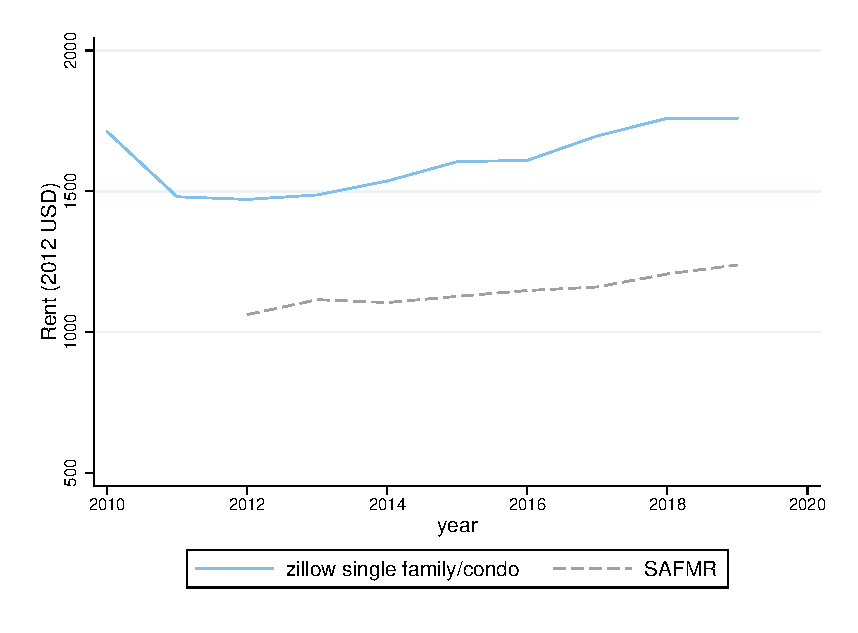
\includegraphics[width = 0.7\textwidth]{../../analysis/zillow_benchmark/output/trend_zillow_safmrwgt_zipcode_avg.eps}
	\begin{minipage}{0.95\textwidth} \footnotesize
		\vspace{3mm}
		\textit{Notes:} The figure plots the annual national average for median	rents in the Single 
		Family, Condos and Condominiums category in Zillow, and a weighted combination of SAFMR series 
		with different number of bedrooms. Weights are based on the US share of single family, 
		condos and cooperative houses with given number of bedrooms as recorded in the \textit{American Housing 
		Survey} (\href{https://www.census.gov/programs-surveys/ahs.html}{AHS}). $\rho = 94.06$ percent. 
		See footnote \ref{foot:zillow_time_series} for details on the construction of this time series.  
	\end{minipage}
\end{figure}

\begin{figure}
	\caption{Comparison Between Zillow Sample and Population Density in CBSAs}
	\label{fig:maps}
	\begin{subfigure}[b]{\textwidth}\centering
		\includegraphics[width = .85\textwidth]{../../analysis/descriptive_maps/output/sample_map.png}
	\end{subfigure}
	\quad 
	\begin{subfigure}[b]{\textwidth}\centering
		\includegraphics[width = .85\textwidth]{../../analysis/descriptive_maps/output/popurban_density_map.png}
	\end{subfigure}
	\begin{minipage}{.95\textwidth} \footnotesize
	\vspace{2mm} 
	\textit{Notes}: Panel (a) shows the geographical location of the zipcodes present in the Zillow SFCC sample 
	used in the main analysis. Summary statistics are reported in \autoref{tab:desc_stats}, column 3. Panel (b) 
	shows the urban population density for the top 100 metropolitan areas in the U.S. as reported in the 2008-2011 
	ACS. Values are winsorized at the 99 percentile to provide enough graphical variation. 
\end{minipage}

\end{figure}

\begin{figure}[!h]
	\caption{Coefficients of dynamic model for different sets of controls}
	\label{fig:}
	\centering
	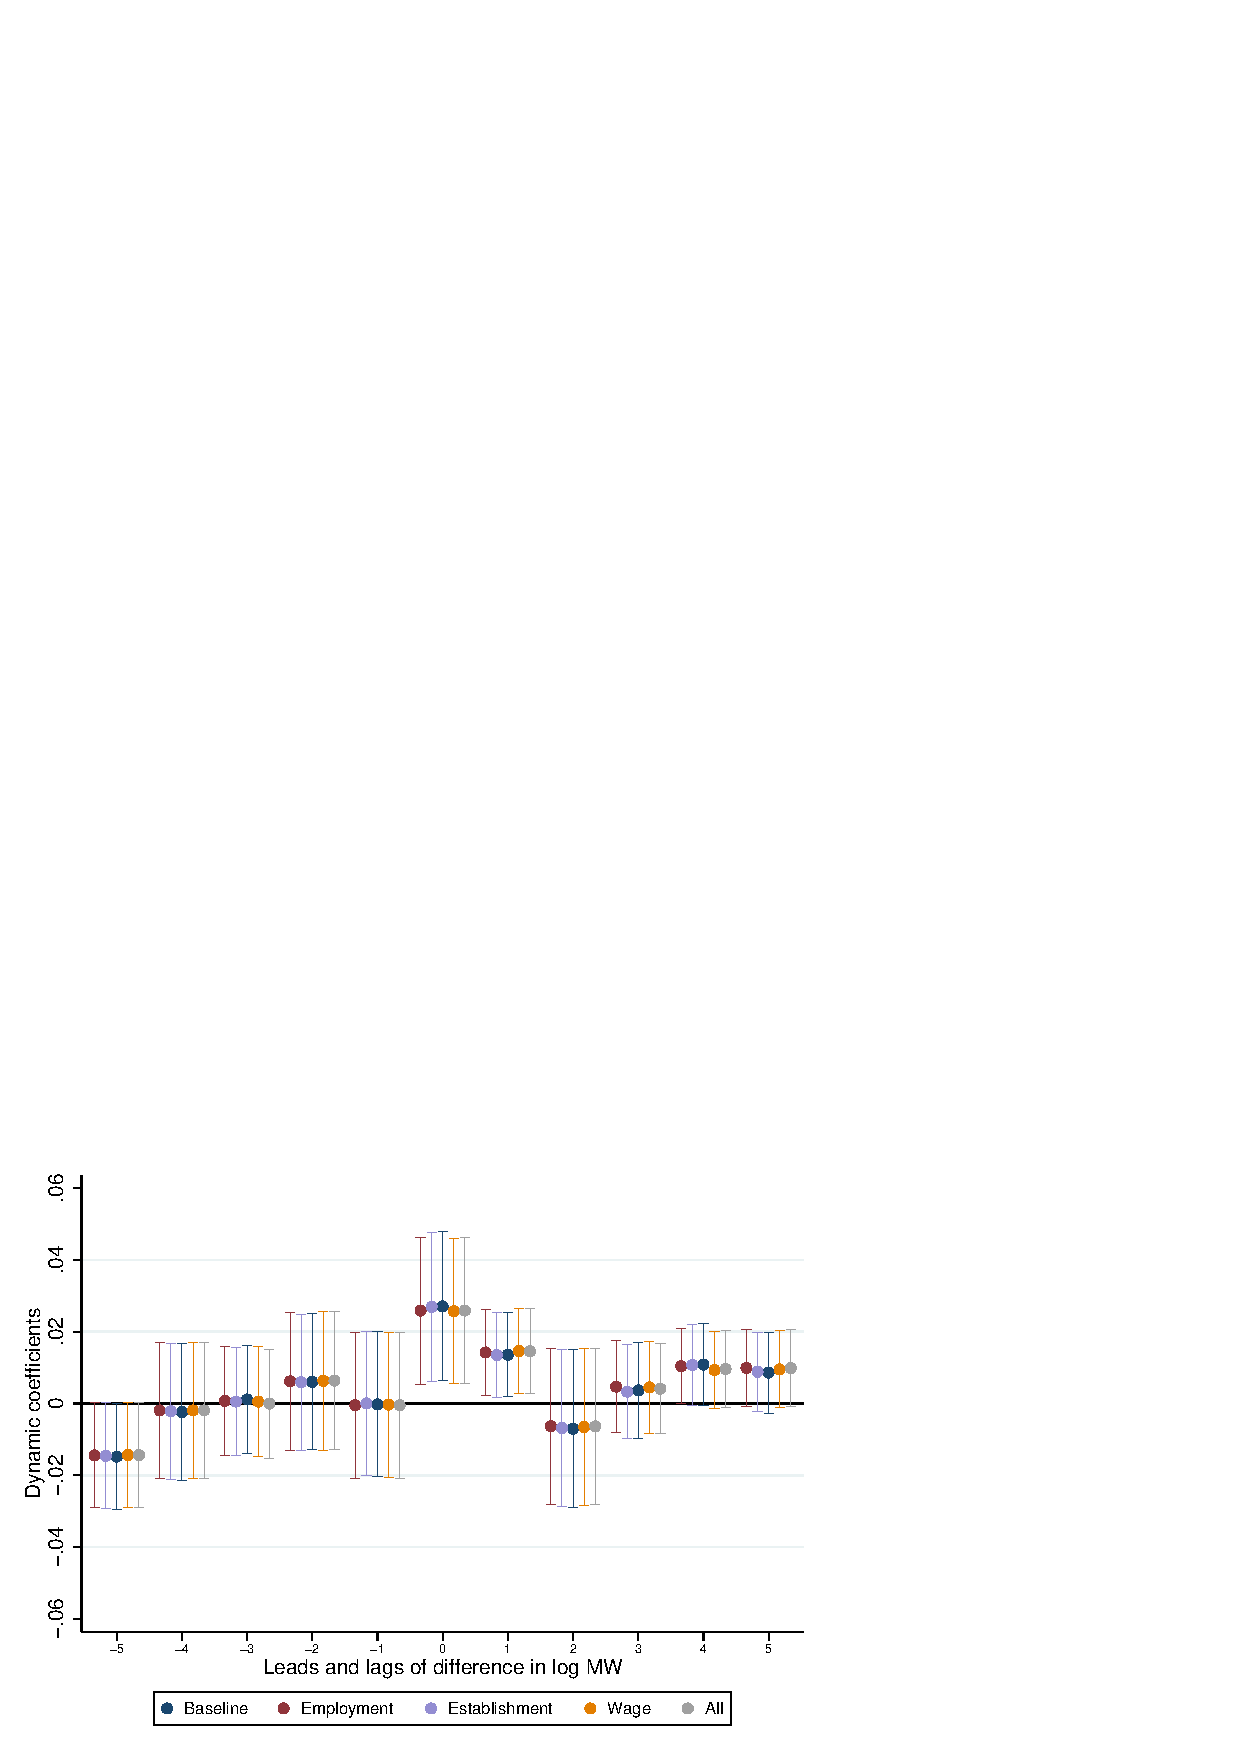
\includegraphics[width = 0.7\textwidth]{../../analysis/first_differences/output/fd_models_control.png}
	\begin{minipage}{.95\textwidth} \footnotesize
		\vspace{2mm} 
		\textit{Notes}: The figure shows the estimated coefficients of the dynamic model defined in 
		equation \autoref{eq:leads_lags} when progressively adding time-varying controls for local shocks. 
		The \textit{baseline} series plots coefficients taken from 
		\autoref{tab:dynamic_lags_leads_main}, column (1). The \textit{employment}, 
		\textit{establishment}, \textit{wage}, and \textit{building} series plot coefficients 
		from \autoref{tab:dynamic_lags_leads_main}, columns (2) to (5) respectively.
		90 percent confidence intervals clustered at the state level reported.
	\end{minipage}
\end{figure}

\begin{figure}[htb!]\centering
	\caption{Placebo Regression with Dependent Variable: (log) Number of SFCCListings for Sale}
	\label{fig:placebo_nlist}
	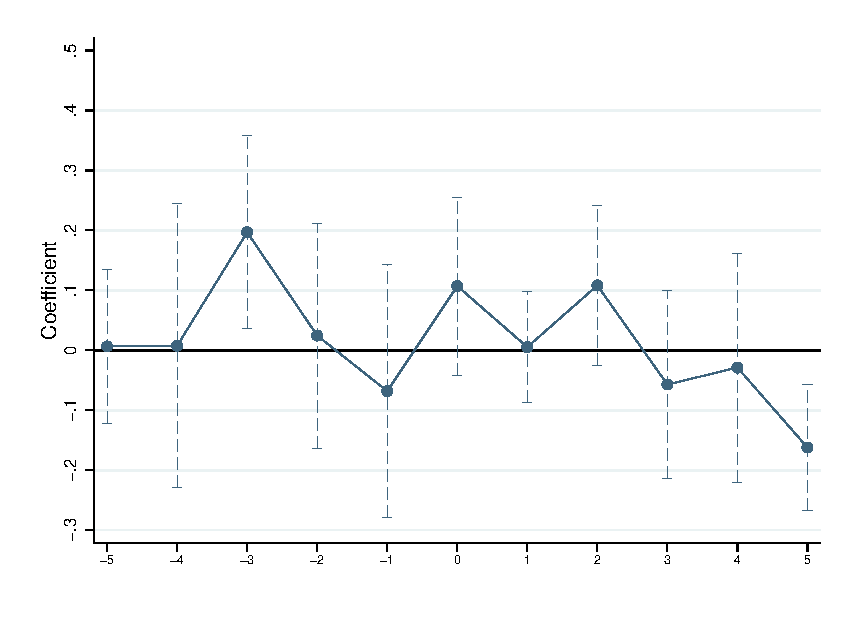
\includegraphics[width = 0.8\textwidth]{../../analysis/first_differences_nlist/output/fd_placebo.eps}	
	\begin{minipage}{\textwidth}\footnotesize
		\textit{Notes:} The figure shows the estimated coefficients of the dynamic model defined in 
		equation \autoref{eq:leads_lags}. The dependent variable is the difference in the natural logarithm 
		of the number of listings \textit{for sale} in the Single Family, Condos, and Cooperative category in 
		Zillow. The model controls for monthly date fixed effects. In addition, it includes 
		economic controls for the industries ``Professional and business services'', 
		``Information'', and ``Financial activities'' from the QCEW. Wage controls are 
		the difference in the natural logarithm of average weekly wages, employment 
		controls are the difference in the natural logarithm of employment, and 
		establishment count controls refer to the difference in the natural logarithm 
		of number of establishments. Wages and employment vary at the county-month level,
		whereas establishment count varies at the country-quarter level.
		90 percent confidence intervals clustered at the state level reported. 
		
	\end{minipage}
\end{figure}

\begin{figure}[htb!]\centering
	\caption{Comparison between Dynamic Baseline Model, Re weighted Model, and Unbalanced-panel Model}
	\label{fig:dynamic_wgt_unabl_comp}
	\begin{subfigure}[b]{0.75\textwidth}
		\caption{Baseline-Re weighted Models}	
		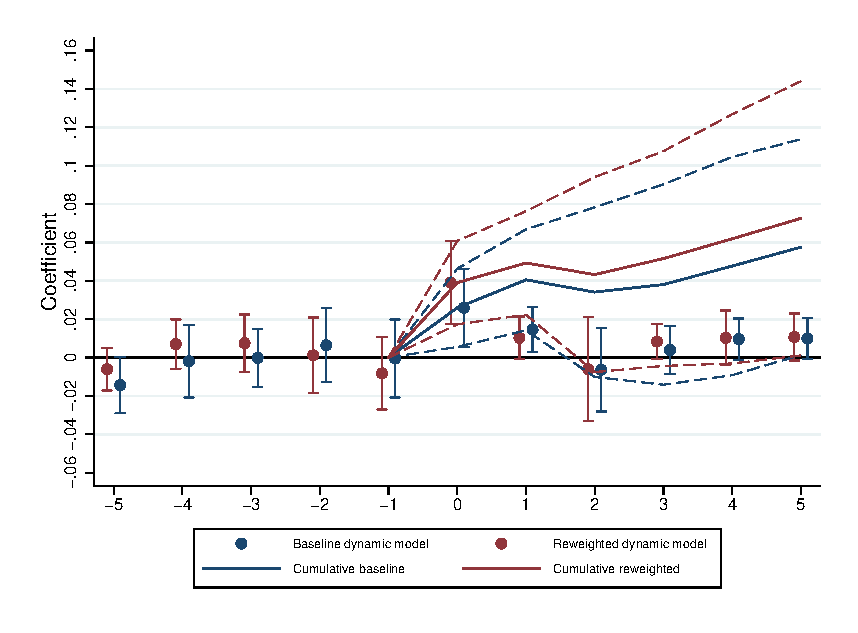
\includegraphics[width = \textwidth]{../../analysis/first_differences_wgt/output/fd_model_comparison_wgt.eps}
	\end{subfigure}
	\quad
	\begin{subfigure}[b]{0.75\textwidth}
		\caption{Baseline-Unbalanced Models}		
		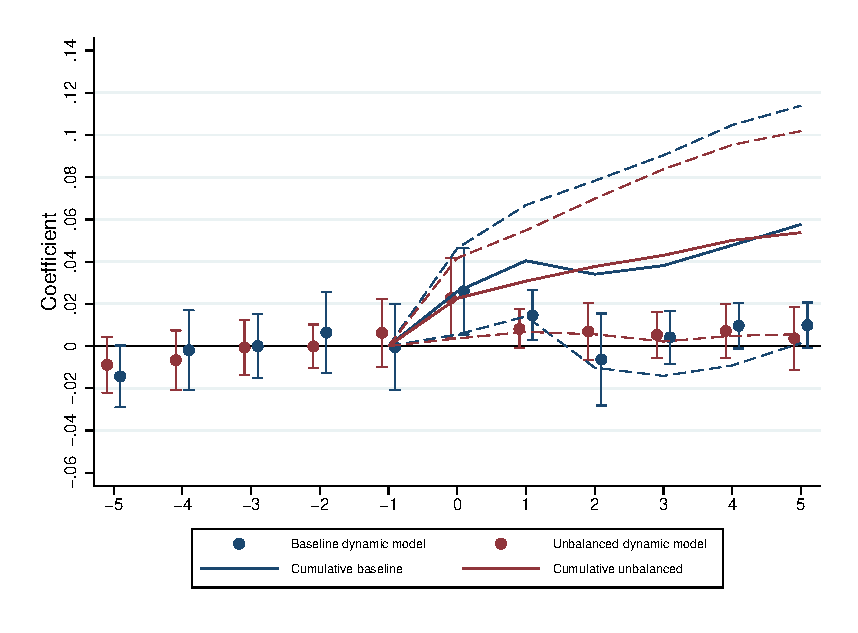
\includegraphics[width = \textwidth]{../../analysis/first_differences_unbal/output/fd_model_comparison_unbal.eps}
	\end{subfigure}
	\begin{minipage}{\textwidth}\footnotesize
		\textit{Notes:} Panel (a) compares estimated coefficients of the dynamic model defined in 
		equation \autoref{eq:leads_lags} obtained from the baseline sample with those obtained from the
		re-weighted sample. Observations are weighted so as to match the average of the 
		following top-100 CBSA characteristics: ``share of rental houses", ``share of African-American residents", 
		``share of college graduates", and ``median income". All characteristics are obtained from 
		the 2010 U.S. Census and the 2008-2011 ACS. See \autoref{sec:sample_rest} for more details. 
		Panel (b)compares estimated coefficients of the dynamic model defined in 
		equation \autoref{eq:leads_lags} obtained from the baseline sample with those obtained using the 
		unbalanced full sample of Zillow zipcodes. The latter model controls for a ``period of entry $\times$
		zipcode" fixed effect. 
		Both panels additionally show, for each model, the cumulative effect obtained by summing up 
		estimates from a distributed lags only specification. 
		All models control for monthly date fixed effects. All models additionally  
		include economic controls from the industries ``Professional and business services'', 
		``Information'', and ``Financial activities'' from the QCEW. Wage controls are 
		the difference in the natural logarithm of average weekly wages, employment 
		controls are the difference in the natural logarithm of employment, and 
		establishment count controls refer to the difference in the natural logarithm 
		of number of establishments. Wages and employment vary at the county-month level,
		whereas establishment count varies at the country-quarter level.
		90 percent confidence interals clustered at the state level reported. 
	\end{minipage}
\end{figure}


\begin{figure}[h!]\centering
	\caption{Distribution for LODES-based Zipcode-level State shares of Minimum Wage Workers and Residents}
	\label{fig:lodes_share_dist}
	\begin{subfigure}[b]{0.8\textwidth}
	\caption{Share of MW Workers}	
	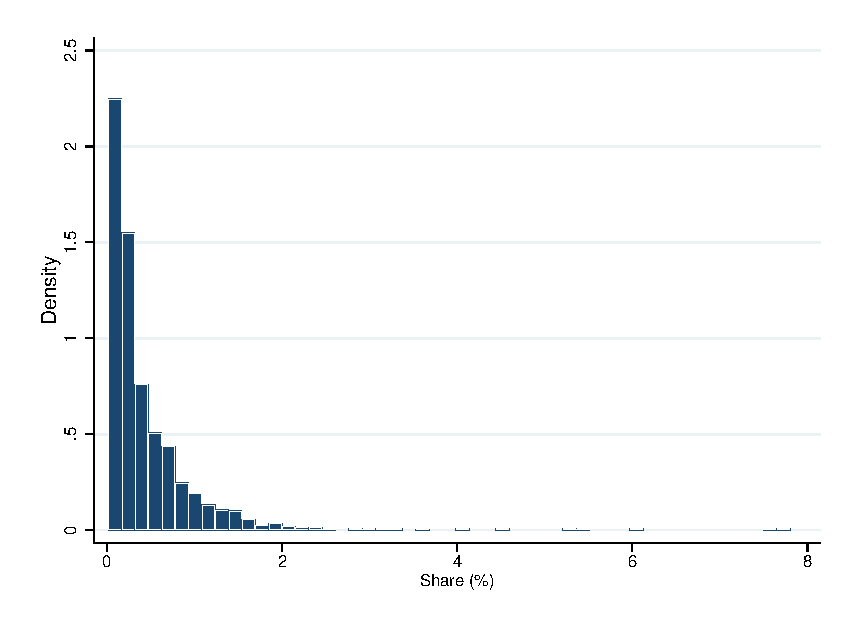
\includegraphics[width = \textwidth]{../../analysis/first_differences_expmw/output/walall_29y_lowinc_ssh_dist.eps}
	\end{subfigure}
	\quad
	\begin{subfigure}[b]{0.8\textwidth}
		\caption{Share of MW Residents}		
		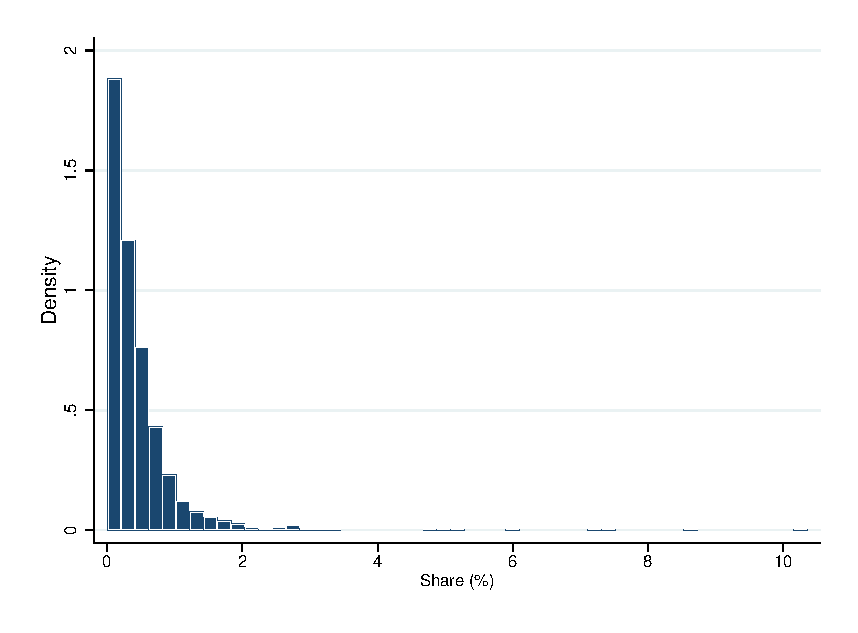
\includegraphics[width = \textwidth]{../../analysis/first_differences_expmw/output/halall_29y_lowinc_ssh_dist.eps}
	\end{subfigure}
	\begin{minipage}{\textwidth}\footnotesize
		\textit{Notes:} Panel (a) shows the distribution for the zipcode-level state share of MW \textit{workers} identified through the LODES data. 
		Panel (b) shows the distribution for the zipcode-level state share of MW \textit{residents} identified through the LODES data. 
		Both shares are computed dividing the number of workers/residents 29 years old or younger earning less than $\$1,250$/month
		by state totals. For more details on the construction of the shares, see \autoref{sec:experienced_mw}.		
	\end{minipage}	
\end{figure}

\begin{figure}[htb!]\centering
	\caption{Estimated static effect of the MW on rents by workplace and residence of young, low-income workers}
	\label{fig:static_qtl_lodes}
	\begin{subfigure}[b]{.5\textwidth}
		\caption{State share, workplace}
		\includegraphics[width = \textwidth]
		{../../analysis/first_differences_expmw/output/fd_static_heter_walall_29y_lowinc_ssh_st_qtl.eps}
	\end{subfigure}%
	\begin{subfigure}[b]{.5\textwidth}
		\caption{State share, residence}
		\includegraphics[width = \textwidth]
		{../../analysis/first_differences_expmw/output/fd_static_heter_halall_29y_lowinc_ssh_st_qtl.eps}
	\end{subfigure}\\
	\begin{subfigure}[b]{.5\textwidth}
		\caption{Zipcode share, workplace}
		\includegraphics[width = \textwidth]
		{../../analysis/first_differences_expmw/output/fd_static_heter_walall_29y_lowinc_zsh_st_qtl.eps}
	\end{subfigure}%
	\begin{subfigure}[b]{.5\textwidth}
		\caption{Zipcode share, residence}
		\includegraphics[width = \textwidth]
		{../../analysis/first_differences_expmw/output/fd_static_heter_halall_29y_lowinc_zsh_st_qtl.eps}
	\end{subfigure}
	\begin{minipage}{\textwidth}\footnotesize
	\vspace{3mm}	
	\textit{Notes:} The figure reports the estimated static effect of MW on rents for different 
	quartile groups across the distribution of young, low-income workers. More precisely, we estimate
	our static model interacting the MW variable with indicators for quartile groups of zipcode-level 
	characteristics, as explained in \autoref{sec:strategy_heterogeneity}. All figures use counts of 
	workplace and residence of young, low-income workers constructed from LODES data. The top 
	row assigns to each zipcode the share of young, low-income workers that work or live there out 
	of state totals. The bottom row constructs a zipcode share of young, low-income workers out of 
	the working population of that zipcode. All models control for monthly date fixed effects. All 
	models additionally include economic controls from the industries ``Professional and business 
	services'', ``Information'', and ``Financial activities'' from the QCEW, as specified throughout
	the paper. 90 percent confidence intervals clustered at the state level reported. 
\end{minipage}
\end{figure}

\begin{figure}[!h]
	\centering
	\caption{Estimated Impact of changes in Experienced MW on changes in Rents - Dynamic DiD model}
	\label{fig:expmw_dynamic}
	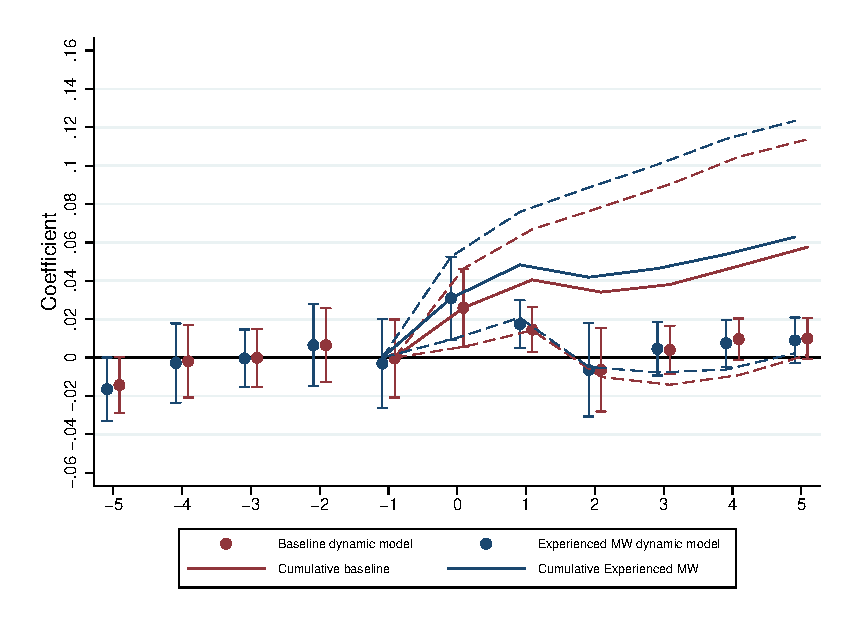
\includegraphics[width = .9\textwidth]{../../analysis/first_differences_expmw/output/fd_model_comparison_expmw.eps}
	\begin{minipage}{.9\textwidth}\footnotesize
		\textit{Notes:} The figure compares estimated coefficients of the dynamic model defined in 
		equation \autoref{eq:leads_lags} obtained from the baseline sample with those obtained when 
		replacing the statutory MW with the experienced MW as main explanatory variable. 
		The plot additionally shows, for each model, the cumulative effect obtained by summing up 
		estimates from a distributed lags only specification. 
		All models control for monthly date fixed effects. All models additionally  
		include economic controls from the industries ``Professional and business services'', 
		``Information'', and ``Financial activities'' from the QCEW. Wage controls are 
		the difference in the natural logarithm of average weekly wages, employment 
		controls are the difference in the natural logarithm of employment, and 
		establishment count controls refer to the difference in the natural logarithm 
		of number of establishments. Wages and employment vary at the county-month level,
		whereas establishment count varies at the country-quarter level.
		90 percent confidence intervals clustered at the state level reported. 
	\end{minipage}
\end{figure}

\clearpage
%%%%%%%%%%%%%%%%%%%%%%%%%%%%%%%%%%%%%%%%%%%%%%%%%%%%%%%%%%%%%%%%%%%%%%%%%%%%%%%%%
\section{A Direct test of the Impact of Minimum Wage on Time-Varying Economic Controls}\label{sec:app_econ_control}
In all the model specifications presented in the paper, we use county-level data from the QCEW 
to control for the local business cycle. However, a potential concern in using local 
economy data may arise if changes in the MW have a \textit{direct} impact on such quantities. This 
would lead the treated and control group be systematically different \parencite{AngristPischke2009}. 

To avoid the ``bad controls" problem, while at the same time including control variables that truly proxy for the 
local economic conditions, we select QCEW county-level time-series for the following industries: "Professional 
and Business Services"; "Information"; and "Finance". According to the Bureau of Labor Statistics (BLS), 
in 2019 such industries accounted for $3.5$, $1$, and $1.2$ percent of the total MW workers respectively, making them 
unlikely to be direcly impacted by MW legislation.\footnote{See the 2020 BLS report on minimum wage workers.} For each 
industry, we observe county-month employment, and county-quarter average weekly wages and establishment count. 

To provide further evidence on the chosen controls' validity, we use them as left-hand side variable in a dynamic DiD
model. The presence of significant pre-treatment trends would suggest how MW react to local economic shocks and
cast doubts on the identification strategy introduced in \autoref{sec:empirical_strategy}. 

QCEW data are aggregated at the county-level, hence preventing us to estimate \autoref{eq:leads_lags}. We therefore 
aggregate MW zipcode-month information at the county-month level by taking, for each period, 
the weighted average of MW levels in each zipcode associated with a given county, using the number of housing units 
as weights. For counties without city-level ordinances, this would simply reflect the state- or county-level MW. Since 
QCEW provides county-month employment data, we are able to estimate the following regression model: 

\begin{equation}
	\label{eq:dynamic_econ_cont_month}
	\Delta y_{ct} = \delta_{t} + \sum\limits_{r=-s}^{s} \beta_r \Delta \underline{w}_{c,t+r} + \Delta \nu_{ct}
\end{equation}

where $y_{ct}$ is the (log) employment in county $c$ in month $t$. The exogeneity 
assumption requires that  $E \left[ \Delta \nu_{ct} | \delta_t, \{ \Delta \underline{w}_{c,t+r} \} \forall r \right] =  0$ 

As for wages and establishment count, the data
is aggregated at the county-quarter level. We hence estimate the impact of the average MW change in a quarter 
over the average rent change. This amounts to running the following regression: 

\begin{equation}
	\label{eq:dynamic_econ_cont_quarter}
	\overline{\Delta y}_{cq} = \overline{\delta}_q +  \sum\limits_{r=-s}^{s} \rho_r \overline{\Delta \underline{w}}_{c,q+r} + \overline{\Delta \nu}_{ct}
\end{equation}

where $\overline{\Delta x}_{cq} = \frac{1}{3} \Delta x_{cq}$ (the quarterly average). Notice that estimating \autoref{eq:dynamic_econ_cont_month} 
and \autoref{eq:dynamic_econ_cont_quarter} is equivalent because the average change over a quarter is a linear combination of 
monthly changes.

ADD PLOTS

%%%%%%%%%%%%%%%%%%%%%%%%%%%%%%%%%%%%%%%%%%%%%%%%%%%%%%%
\section{A toy model of the local housing market}\label{sec:model}

We build a simple model that is used to build a benchmark estimate of the effect of MW
policies on rents.

\subsection{Model set-up}

We focus on the supply and demand of housing in a given zipcode. Consider an environment with 
an exogenously given continuum of households in each zipcode divided in two groups: minimum wage 
and non-minimum wage households (HH). The former are fully affected by the MW, whereas the latter 
are not affected at all.

On the supply side, we denote by $H$ the continuous measure of housing units available for rent 
in the zipcode. We assume that units are homogeneous, and can be rented at the a rent of $r$. The 
supply of housing $H(r)$ is assumed to be increasing in rents $r$, so that $H'(r) > 0$.

Let us move to the demand side. Households receive monthly a income, which we denote by 
$\underline{w}$ and $w$ for MW HH and non-MW households, respectively. Demand for housing is given 
by $\underline{H}(r, \underline{w})$ and $\overline{H}(r, w)$ for each household type. We make two 
standard assumptions on these objects: (i) the demand of housing is downward sloping (i.e., 
$\underline{H}_r(r, \underline{w}) < 0$ and $\overline{H}_r(r, w) < 0$); and (ii) the demand for 
housing is increasing in income (i.e., $\underline{H}_w(r, \underline{w}) > 0$ and $\overline{H}_w(r, 
w) > 0$)


\subsection{Equilibrium and the elasticity of rents to the minimum wage}

Equilibrium rents $r^*$ are such that local housing supply is equated to local housing demand. 
Formally,

\begin{equation*}\label{eq:model-eq}
H(r) =  \underline{H}(r, \underline{w}) + \overline{H}(r, w) \ .
\end{equation*}

We are interested in the elasticity of equilibrium rents $r^*$ to the minimum wage $\underline{w}$, 
which we denote by $\rho$. The implicit function theorem applied on the above equation yields

\begin{equation}\label{eq:model-elasticity}
\rho := \frac{d \ln r^*}{d \ln \underline{w}} 
= \frac{\underline{w} \ \underline{H}_w}
{r\  H'(r) - r \ \underline{H}_r - r \ \overline{H}_r} \ ,
\end{equation}
where we denote partial derivatives with sub-indexes.

Note that, since $\underline{H}_r < 0$ and $\overline{H}_r < 0$, the above expression is always 
positive. When the MW increases the local housing market moves to a new equilibrium with higher 
rents. The magnitude of the elasticity is driven by the relative magnitudes of the earnings of 
minimum wage workers ($\overline{w}$) and rents ($r$), and the slopes of the different 
functions in equilibrium. For instance, a higher response of housing demand to the minimum wage 
change ($\underline{H}_w$) would result in a higher elasticity.

\clearpage
%%%%%%%%%%%%%%%%%%%%%%%%%%%%%%%%%%%%%%%%%%%%%%%%%%%%%%%%%%%%%%%%%%%%%%%%%%%%%%%%
\section{Additional Tables and Figures}

\begin{table}[hbt!] \centering
    \caption{Summary statistics of baseline panel}
    \label{tab:stats_est_panel}
    \begin{tabular}{@{}lccccc@{}}
        \toprule
                                          & \multicolumn{1}{c}{N} 
                                          & \multicolumn{1}{c}{Mean} 
                                          & \multicolumn{1}{c}{St. Dev.} 
                                          & \multicolumn{1}{c}{Min} 
                                          & \multicolumn{1}{c}{Max}                 \\ \midrule
        \textit{Minimum wage variables}               &       &       &       &       &       \\
        $\quad$Statutory MW $\MW_{it}$                & 80,700  & 8.56  & 1.58  & 7.25  & 16.00  \\
        $\quad$Residence MW $\mw^{\res}_{it}$         & 80,700  & 2.132  & 0.168  & 1.981  & 2.773  \\
        $\quad$Workplace MW $\mw^{\wkp}_{it}$         & 80,700  & 2.136  & 0.163  & 1.981  & 2.694  \\
        $\quad$Workplace MW, low-income workers       & 80,700  & 2.134  & 0.161  & 1.981  & 2.681  \\
        $\quad$Workplace MW, young workers            & 80,700  & 2.135  & 0.163  & 1.981  & 2.707  \\[.3em]
        \textit{Median Rents}                         &       &       &       &       &       \\
        $\quad$SFCC                                   & 74,012  & 1,757.89  & 901.50  & 625.00  & 30,000.00  \\
        $\quad$SFCC per sqft.                         & 80,700  & 1.32  & 1.01  & 0.47  & 22.20  \\
        $\quad$Log(SFCC per sqft.)                    & 80,700  & 0.14  & 0.47  & -0.76  & 3.10  \\[.3em]
        \textit{Economic controls}                    &       &       &       &       &       \\
        $\quad$Avg.\ wage Business services           & 80,700  & 11.19  & 1.38  & 6.02  & 13.39  \\
        $\quad$Employment Business services           & 80,700  & 8.71  & 1.25  & 4.36  & 10.96  \\
        $\quad$Estab. count Business services         & 80,700  & 7.14  & 0.31  & 5.73  & 8.18  \\
        $\quad$Avg.\ wage Financial services          & 80,352  & 9.01  & 1.57  & 2.40  & 12.39  \\
        $\quad$Employment Financial services          & 80,700  & 6.13  & 1.35  & 1.61  & 9.53  \\
        $\quad$Estab. count Financial services        & 80,352  & 7.33  & 0.36  & 5.89  & 8.91  \\
        $\quad$Avg.\ wage Information services        & 80,688  & 10.23  & 1.43  & 4.75  & 12.90  \\
        $\quad$Employment Information services        & 80,700  & 8.01  & 1.21  & 3.66  & 10.34  \\
        $\quad$Estab. count Information services      & 80,688  & 7.31  & 0.37  & 6.33  & 9.16  \\ \bottomrule
    \end{tabular}

    \begin{minipage}{.95\textwidth} \footnotesize
        \vspace{2mm}
        Notes: This table shows summary statistics of the panel of ZIP codes 
        used in our baseline results, constructed as explained in Section 
        \ref{sec:data_final_panel}.
        All workplace MW variables use 2017 commuting data from LODES.
        The workplace MW variables ``Workplace MW, low-income workers'' and 
        ``Workplace MW, young workers'' are constructed using data for 
        workers who earn less \$1,251 and are aged less than 29, respectively.
    \end{minipage}
\end{table}

\clearpage
\begin{table}[hbt!] \centering
    \caption{Estimates of the effect of the MW on rents in levels and first differences,
             baseline sample}
    \label{tab:autocorrelation}
    \begin{tabular}{@{}lcc@{}}
        \toprule
            & \multicolumn{2}{c}{Log rents}                             \\ \cmidrule(l){2-3} 
            & \shortstack{Levels\\(1)} 
            & \shortstack{First Differences\\(2)}                       \\ \midrule
        Residence minimum wage             &  0.0740   &  -0.0207              \\
                                           & (0.2221)  & (0.0171)             \\
        Workplace minimum wage             &  -0.0524   &  0.0546              \\
                                           & (0.2226)  & (0.0281)             \\ \midrule
        County-quarter economic controls   &  Yes   &  Yes              \\
        P-value autocorrelation test       &        &  $<0.0001$        \\
        R-squared                          &  0.9889   &  0.0209              \\
        Observations                       &  132,897  &  131,383             \\ \bottomrule
    \end{tabular}

    \begin{minipage}{.95\textwidth} \footnotesize
        \vspace{2mm}
        \textit{Notes}: 
        Data are from the baseline estimation sample described in Section 
        \ref{sec:data_final_panel}.
        Both columns report the results of regressions of the log of 
        median rents per square foot on our MW-based measures.
        Column (1) presents estimates of a model in levels, including 
        ZIP code and year-month fixed effects.
        Column (2), presents estimates of a model in first differences, 
        including year-month fixed effects 
        (note that the ZIP code fixed effect drops out).
        For the model in first differences, we also report the results of an 
        AR(1) auto-correlation test.
        We proceed as in \parencite[][Section 10.6.3]{wooldridge2010}.
        First, we compute the residuals of the model estimated in column (2), 
        and we regress those residuals on their lag.
        Let the auto-correlation coefficient of this model be $\rho$.
        The model in levels is efficient assuming no auto-correlation in the 
        error term, which would imply that the residuals of the 
        first-differenced model are auto-correlated with $\rho = -0.5$.
        The row ``P-value autocorrelation test'' reports the $p$-value of 
        a Wald test of that hypothesis.
    \end{minipage}
\end{table}

\clearpage
\begin{table}[hbt!] \centering
    \caption{Stacked model}
    \label{tab:stacked_w6}
    \begin{tabular}{l*{4}{c}}
        \toprule
        & \multicolumn{1}{c}{\shortstack{Change in wrk.\\MW $\Delta\mw_{it}^{\wkp}$}}
            & \multicolumn{3}{c}{\shortstack{Change in log rents\\$\Delta r_{it}$}} \\ \cmidrule(lr){2-2}\cmidrule(lr){3-5}
                                            & (1)   & (2)   & (3)   & (4)            \\ \midrule
        Change in residence MW 
                    $\Delta\mw_{it}^{\res}$  &  0.5331  &  0.0076  &       &  -0.0265     \\
                                            & (0.0337) & (0.0129) &       & (0.0204)    \\
        Change in workplace MW 
                    $\Delta\mw_{it}^{\wkp}$ &       &       &  0.0237  & 0.0639      \\
                                            &       &       & (0.0226) & (0.0349)    \\ \midrule
        Sum of coefficients                &       &       &       &  0.0375     \\
                                            &       &       &       & (0.0238)    \\ \midrule
        County-quarter economic controls   &  Yes  & Yes   & Yes   & Yes      \\
        P-value equality                   &       &       &       & 0.0932      \\
        R-squared                          &  0.9769  &  0.0817  &  0.0817  & 0.0817      \\
        Observations                       & 110,239  & 110,239  & 110,239  & 110,239     \\\bottomrule
    \end{tabular}

    \begin{minipage}{.95\textwidth} \footnotesize
        \vspace{2mm}
        Notes: 
        Data are from the baseline estimation sample described in Section 
        \ref{sec:data_final_panel}.
        The table mimicks the estimates in Table \ref{tab:static} but using a 
        ``stacked'' sample.
        To construct the sample we proceed as follows.
        First, we define a CBSA-month as treated if in that month there is at 
        least one ZIP code that had a change in the binding MW.
        For each of the selected CBSA-months we assign a unique event ID. 
        Second, for each event we take a window $w = 6$, and we keep all months 
        within that window for the ZIP codes that belong to the treated CBSA.
        If a ZIP code has missing data for some month within the window, we drop 
        the entire ZIP code from the respective event.
        For each column, we estimate the same model as the analogous column in 
        Table \ref{tab:static} but include event indicator $\times$ year-month
        fixed effects.
    \end{minipage}
\end{table}

\clearpage
\begin{table}[hbt!]
    \centering
    \caption{Estimates of the effect of the MW on rents including one lag of the 
             dependent variable, baseline sample}
    \label{tab:static_ab}

    \begin{tabular}{@{}lcc@{}}
        \toprule
                               & \multicolumn{2}{c}{\shortstack{Change log rents $\Delta r_{it}$}}  \\ \cmidrule(l){2-3}
                               & \shortstack{Baseline\\(1)} & \shortstack{Arellano-Bond\\(2)} \\ \midrule
        Change residence MW 
                  $\Delta\mw_{it}^{\res}$  &  #4#           &  #4#                           \\
                                           & (#4#)          & (#4#)                          \\
        Change workplace MW 
                   $\Delta\mw_{it}^{\wkp}$ &  #4#           & #4#                            \\
                                           & (#4#)          & (#4#)                          \\
        Lagged change log rents 
                   $\Delta r_{i,t-1}$      &                & #4#                            \\
                                           &                & (#4#)                          \\ \midrule
        County-quarter economic controls   & Yes            & Yes                            \\
        P-value equality                   & #4#            & #4#                            \\
        Observations                       & #0,#           & #0,#                           \\ \bottomrule
    \end{tabular}

    \begin{minipage}{.95\textwidth} \footnotesize
        \vspace{2mm}
        Notes: 
        Data are from the baseline estimation sample described in Section 
        \ref{sec:data_final_panel}.
        Both columns show the results of regressions of the log of 
        median rents per square foot on our MW-based measures.
        Column (1) repeats the results of Column (4) in Table \ref{tab:static}.
        Column (2) extends the estimate of Column (2) including the lagged 
        change in log rents as a control, and is estimated using an 
        instrumental-variables strategy that uses the second lag of rents
        as an instrument for the first lag following \textcite{ArellanoBond1991}.
        All regressions are estimated in first differences and include 
        time-period fixed effects and economic controls that vary at the 
        county and month levels.
        The measure of rents per square foot corresponds to the Single Family, 
        Condominium and Cooperative houses from Zillow.
        The residence MW is defined as the log statutory MW in the same ZIP code.
        The workplace MW is defined as the statutory MW where the average 
        resident of the ZIP code works, constructed using LODES 
        origin-destination data.
        Economic controls from the QCEW include the log of the average wage, 
        the log of employment, and the log of the establishment count from the 
        sectors ``Information'', ``Financial activities'', and ``Professional
        and business services''.
        Standard errors in parentheses are clustered at the state level.
    \end{minipage}
\end{table}

\clearpage
\begin{landscape}
\begin{table}[ht!]
    \centering
    \caption{Comparison of estimates of the effect of the MW on rents, different
             Zillow categories}
    \label{tab:zillow_categories}
        
    \begin{tabular}{@{}lccccc@{}}
        \toprule
                                             & \multicolumn{1}{c}{\shortstack{Change wkp.\ MW\\$\Delta\mw_{it}^{\wkp}$}} 
                                             & \multicolumn{3}{c}{\shortstack{Change log rents\\$\Delta r_{it}$}}
                                             &                                                                         \\ \cmidrule(lr){2-2}\cmidrule(lr){3-5}
                                                 & \multicolumn{1}{c}{\shortstack{Change res.\ MW\\$\Delta\mw_{it}^{\res}$}}
                                                 & \multicolumn{1}{c}{\shortstack{Change res.\ MW\\$\Delta\mw_{it}^{\res}$}} 
                                                 & \multicolumn{1}{c}{\shortstack{Change wkp.\ MW\\$\Delta\mw_{it}^{\wkp}$}} 
                                                 & \shortstack{Sum of\\coefficients} 
                                                 & N                                    \\ \midrule
        $\quad$(a) Unbalanced (SFCC)             &  0.8471  &  -0.0254  &  0.0471  &  0.0218  & 193,292 \\
                                                 & (0.0301) & (0.0210) & (0.0309) & (0.0161) &      \\
        $\quad$(b) Single family (SF)            &  0.8591  &  -0.0133  &  0.0385  &  0.0252  & 140,750 \\
                                                 & (0.0319) & (0.0392) & (0.0471) & (0.0140) &      \\
        $\quad$(c) Condo/Cooperatives (CC)       &  0.8010  &  -0.0682  &  0.0975  &  0.0293  & 29,817 \\
                                                 & (0.0291) & (0.0288) & (0.0427) & (0.0187) &      \\
        $\quad$(d) Studio                        &  0.8330  &  -0.0666  &  0.0772  &  0.0107  & 22,746 \\
                                                 & (0.0287) & (0.0520) & (0.0570) & (0.0207) &      \\
        $\quad$(d) 1 Bedroom                     &  0.7863  &  0.0284  &  -0.0336  &  -0.0052  & 53,538 \\
                                                 & (0.0303) & (0.0266) & (0.0456) & (0.0212) &      \\
        $\quad$(e) 2 Bedroom                     &  0.7999  &  -0.0054  &  0.0043  &  -0.0011  & 89,635 \\
                                                 & (0.0297) & (0.0232) & (0.0286) & (0.0117) &      \\
        $\quad$(f) 3 Bedroom                     &  0.8103  &  -0.0634  &  0.0920  &  0.0287  & 64,916 \\
                                                 & (0.0325) & (0.0472) & (0.0684) & (0.0334) &      \\
        $\quad$(g) Multifamily 5+ units          &  0.8056  &  -0.0137  &  0.0378  &  0.0241  & 142,759 \\
                                                 & (0.0316) & (0.0260) & (0.0362) & (0.0116) &      \\ \bottomrule
    \end{tabular}

    \begin{minipage}{.95\linewidth} \footnotesize
        \vspace{2mm}
        Notes:
        Data are from Zillow \parencite{ZillowData}, 
        the statutory MW panel described in Section \ref{sec:data_mw_panel}, 
        LODES origin-destination statistics \parencite{CensusLODES},
        and the QCEW \parencite{QCEW}.
        Each row of the table shows two estimations on the same sample of ZIP 
        codes and months.
        The first column shows the results of a regression of the change in the 
        workplace MW measure on the change in the residence MW measure.
        The second through fourth columns show the results of a regression of 
        the change in log rents on the change in the residence MW and the 
        workplace MW, with the fifth column showing the sum of the coefficients 
        on the MW measures.
        All rent variables correspond to the median per square foot rent in a 
        Zillow category.
        All estimated regressions include fixed effects for each year-month and 
        economic controls at the county $\times$ quarter level from the QCEW.
        Row (a) repeats the results of column (5) of Table \ref{tab:static_sample}, 
        using the Single Family, Condominium and Cooperative Houses category.
        Rows (b) through (g) estimate the same regression for different Zillow 
        categories.
        We exclude the rental categories ``4 Bedroom,'' ``5 bedroom,'', and 
        ``Duplex and triplex,'' all of which contain less than 15 thousand
        ZIP code by month observations.
        Standard errors in parentheses are clustered at the state level.
    \end{minipage}
\end{table}
\end{landscape}

\clearpage
\begin{landscape}
\begin{table}[ht!]
    \centering
    \caption{Comparison of estimates of the effect of the MW on rents across 
             geographies and time frames}
    \label{tab:static_geos_times}
    
    \begin{tabular}{@{}lccccc@{}}
        \toprule
                                                         & \multicolumn{1}{c}{\shortstack{Change workplace\\MW $\Delta\mw_{it}^{\wkp}$}} 
                                                         & \multicolumn{3}{c}{\shortstack{Change log rents\\$\Delta r_{it}$}}
                                                         &                                                                         \\ \cmidrule(lr){2-2}\cmidrule(lr){3-5}
                                                             & \multicolumn{1}{c}{\shortstack{Change residence\\MW $\Delta\mw_{it}^{\res}$}}
                                                             & \multicolumn{1}{c}{\shortstack{Change residence\\MW $\Delta\mw_{it}^{\res}$}}
                                                             & \multicolumn{1}{c}{\shortstack{Change workplace\\MW $\Delta\mw_{it}^{\wkp}$}} 
                                                             & \shortstack{Sum of\\coefficients}
                                                             & N                                                                    \\ \midrule
        \textit{Panel A: Baseline (ZIP code $\times$ Month)}          &       &       &       &       &      \\
        $\quad$(i) Residence MW only                         &       &  0.0345  &       &       & 90,255 \\
                                                             &       & (0.0141) &       &       &      \\
        $\quad$(ii) Workplace MW only                        &       &       &  0.0411  &       & 90,255 \\
                                                             &       &       & (0.0154) &       &      \\
        $\quad$(iii) Both residence and workplace MW         &  0.8661  &  -0.0158  &  0.0581  &  0.0423  & 90,255 \\
                                                             & (0.0333) & (0.0164) & (0.0262) & (0.0155) &      \\
        \textit{Panel B: County $\times$ Month}              &       &       &       &       &      \\
        $\quad$(i) Residence MW only                         &       &  0.0157  &       &       & 31,767 \\
                                                             &       & (0.0168) &       &       &      \\
        $\quad$(ii) Workplace MW only                        &       &       &  0.0207  &       & 31,767 \\
                                                             &       &       & (0.0190) &       &      \\
        $\quad$(iii) Both residence and workplace MW         &  0.8801  &  -0.0414  &  0.0649  &  0.0235  & 31,767 \\
                                                             & (0.0222) & (0.0280) & (0.0368) & (0.0193) &      \\
        \textit{Panel C: ZIP code $\times$ Year}             &       &       &       &       &      \\
        $\quad$(i) Residence MW only                         &       &  0.0221  &       &       & 7,745 \\
                                                             &       & (0.0526) &       &       &      \\
        $\quad$(ii) Workplace MW only                        &       &       &  0.0231  &       & 7,745 \\
                                                             &       &       & (0.0573) &       &      \\
        $\quad$(iii) Both residence and workplace MW         &  0.9006  &  0.0260  &  -0.0044  &  0.0216  & 7,745 \\
                                                             & (0.0242) & (0.1136) & (0.1279) & (0.0573) &      \\ \bottomrule
    \end{tabular}
    
    \begin{minipage}{.95\linewidth} \footnotesize
        \vspace{2mm}
        Notes:
        Data are from the baseline estimation sample described in Section 
        \ref{sec:data_final_panel}, where we select ZIP codes and counties based 
        on whether they had non-missing values of median rents per square foot 
        in the SFCC category in Zillow as of July 2015.
        The first column and rows labeled (iii) show the results of a regression 
        of the change in the workplace MW measure on the change in the 
        residence MW measure.
        The second through fourth columns show the results of regressions of the 
        change in log rents on either the change in the residence MW---rows (i)---
        or the workplace MW---rows (ii)--- 
        or both---rows (iii)---, with the fifth column showing the sum of the 
        coefficients on the MW measures.
        The last column shows the number of observations, fixed within each row.
        All regressions include economic controls from the QCEW, as defined in
        Table \ref{tab:static}.
        Regressions estimated at a yearly frequency use the yearly average of
        the change in the MW measures and the change in the economic controls.
        Panel A repeats our baseline results from Table \ref{tab:static}, where 
        the unit of observation is the ZIP code $\times$ month.
        Panel B shows results for a panel where the unit of observation is the 
        county $\times$ month.
        Panel C shows results for a panel where the unit of observation is the 
        ZIP code $\times$ year.
        In all panels,
        (i) displays the results of a regression of the change in log rents on 
        the residence MW only;
        (ii) displays the results of a regression of the change in log 
        rents on the workplace MW only; and
        (iii) displays the results of a regression of the change in workplace
        MW on the change in residence MW (column 1), and of the change in 
        log rents on both MW measures (columns 2--5).
        Standard errors in parentheses are clustered at the state level.
    \end{minipage}
\end{table}
\end{landscape}

\clearpage
\begin{table}[]
    \caption{Estimates of the effect of minimum wage on income}
    \label{tab:static_wages}

    \begin{tabular}{@{}lccccc@{}}
        \toprule
                                        & \multicolumn{5}{c}{Log wage bill}                         \\ \cmidrule(l){2-6} 
                                        & (1)       & (2)      & (3)      & (4)      & (5)          \\ \midrule
        Workplace minimum wage             & -0.0385    & -0.0370   & 0.0198   & 0.0736      & -0.0287     \\
                                        & (0.1985)  & (0.1630) & (0.0894) & (0.3333)    & (0.2214)   \\ \midrule
        Sample                             & All       & All      & All      & All       & Baseline     \\
        County-level economic controls     & No        & Yes      & Yes      & Yes       & Yes          \\
        Geographical non-parametric trends & No        & No       & CBSA     & County     & CBSA         \\
        Within R-squared                   & 0.1341   & 0.1031   & 0.0726   & 0.0326     & 0.1802        \\
        Observations                       & 0   & 0  & 0  & 0    & 0       \\ \bottomrule
    \end{tabular}
    
    \begin{minipage}{.95\textwidth} \footnotesize
        \vspace{2mm}
        Notes: The table shows different estimations for the effect of the workplace minimum 
        wage on a ZIP code's log wage bill.
        The workplace minimum wage is the average in the year of the workplace minimum wage 
        defined in Section XX, using constant commuting shares as of 2017.
        Column (1) shows a two-way fixed effects model with no controls, where the fixed 
        effects are given by ZIP code and year.
        Column (2) adds the average in the year of the county-quarter economic controls from
        QCEW.
        Column (3) expands the model from column (2) interacting the year fixed effects 
        with CBSA indicators.
        Column (4) expands the model from column (2) interacting the year fixed effects 
        with county indicators.
        Column (5) uses the specification in column (4) on our baseline sample of ZIP codes,
        uses in Table \ref{tab:static}.
    \end{minipage}
\end{table}


\clearpage
\begin{table}[hbt!]
    \centering
    \caption{AVerage effect of an increase in federal MW to \$7.97 and to \$15 
             in January 2020, urban ZIP codes}
    \label{tab:counterfactuals_other}

    \begin{tabular}{@{}lccccc@{}}
        \toprule
                         & N & \shortstack{Change in\\res.\ MW}
                             & \shortstack{Change in\\wkp.\ MW}
                             & \shortstack{Share of\\housing exp.}  
                             & \shortstack{Share\\Pocketed}                      \\ \midrule
        \textit{Panel A: Fed.\ MW to \$7.97}         &      &       &       &     &      \\
        $\quad $Effect in ZIP codes with...          &      &       &       &     &      \\
        $\quad \quad$previous MW $\leq\$7.97\quad$   & #0,# &  #3# & #3#  & #3# &  #3#   \\
        $\quad \quad$previous MW $>\$7.97\quad$      & #0,# &  #0# & #3#  & #3# & #3#    \\[.3em]
        \textit{Panel B: Fed.\ MW to \$15}           &      &       &       &     &      \\
        $\quad $Effect in ZIP codes with...          &      &       &       &     &      \\
        $\quad \quad$previous MW $\leq\$15\quad$     & #0,# &  #3# & #3#  & #3# &  #3#   \\
        $\quad \quad$previous MW $>\$15\quad$        & #0,# &  #0# & #3#  & #3# & #3#    \\ \bottomrule
    \end{tabular}
    
    \begin{minipage}{.95\textwidth} \footnotesize
        \vspace{2mm}
        Notes: 
        Data are from LODES and the minimum wage panel described in Section 
        \ref{sec:mw_construction}.
        The table shows averages of the estimated ZIP-code specific shares of the 
        additional income pocketed by landlords (``Share pocketed''), 
        defined as the ratio of the increase in income to the increase in rents.
        We also report the average 
        change in residence MW, change in workplace MW,
        and share of ZIP-code specific housing expenditure 
        (``Avg.\ share of housing exp.'') defined as explained in XXXX.
        Increases in income and rents are simulated following the procedure 
        described in Section \ref{sec:counterfactual}.
        Panel A assumes a 10\% increase in the federal MW, and
        Panel B assumes an increase in the federal MW to \$15.
        We assume the following parameter values:
        $\beta = \betaCounterfactual$, $\gamma = \gammaCounterfactual$, and $\varepsilon = \epsilonCounterfactual$.
        We carry out our computations only for urban ZIP codes, defined as 
        those that belong to a CBSA with at least 80\% of urban population
        according to the 2010 census.
        The figure excludes ZIP codes located in CBAs for which the average
        estimated change in log total wages was below 0.1\% in the respective
        counterfactual scenario.
    \end{minipage}
\end{table}


\clearpage

\begin{figure}[h!]
    \centering
    \caption{Sample of ZIP codes in Zillow data and population density, mainland US}
    \label{fig:map_zillow_sample}

    \begin{subfigure}{1\textwidth}
        \centering
        \caption{Zillow ZIP codes}
        \includegraphics[width = 0.95\textwidth]
            {maps_US/output/USPS_zipcodes_zillow_data.png}
    \end{subfigure}\\
    \begin{subfigure}{1\textwidth}
        \centering
        \caption{Population Density}
        \includegraphics[width = 0.95\textwidth]
            {maps_US/output/USPS_zipcodes_pop_density.png}
    \end{subfigure}

    \begin{minipage}{.95\textwidth} \footnotesize
        \vspace{3mm}
        Notes:
        Data are from \textcite{ZillowData} and \textcite{ESRI}.
        The figure compares the USPS ZIP codes available in Zillow to the 
        population density.
        Panel (a) shows the sample of the ZIP codes that have rents data in 
        the SFCC category at any point in the period 2010--2019.
        Panel (b) shows quintiles of population density according to the
        2010 US Census, and measured in population per square mile.
    \end{minipage}
\end{figure}

\clearpage

\begin{figure}[h!]
    \centering
    \caption{Time trends in rents according to Zillow and SAFMR}
    \label{fig:trend_zillow_safmr}

	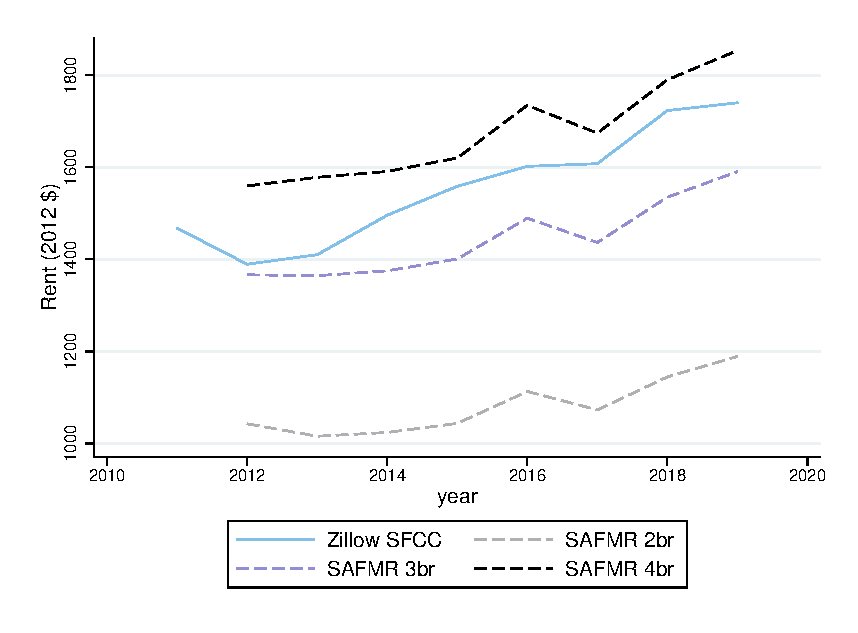
\includegraphics[width = 0.7\textwidth]
        {zillow_benchmark/output/trend_zillow_safmr_zipcode_m1.png}
    %%
    %%  SH: This figure (and folder in general) needs a review. 
    %%      - Format should be dps
    %%      - Legend should fit better, and change 'zillow' --> 'Zillow'
    %%      - We should drop figures we don't need
    %%

    \begin{minipage}{.95\textwidth} \footnotesize
        \vspace{3mm}
        Notes:
        Data are from \textcite{ZillowData} and Small Area Fair Market Rents 
        (\citeyear[SAFMR]{hudSAFMR}).
        The figure compares the evolution of the median rental value in Zillow
        to three SAFMRs series, for 2, 3, and 4 or more bedrooms.
    \end{minipage}
\end{figure}

\clearpage
\begin{figure}[h!]
    \centering
    \caption{Spatial distribution of minimum wage changes, mainland US}
    \label{fig:map_mw_perc_changes}

    \includegraphics[width = 1\textwidth]
        {maps_mw_long_run/output/USchange_perc_statutory_mw.png}

    \begin{minipage}{.95\textwidth} \footnotesize
        \vspace{3mm}
        Notes: 
        Data are from the MW panel described in
        Section \ref{sec:data_mw_panel}.
        The figure maps the percentage change in the statutory MW
        level in each ZIP code from January 2010 to December 2019.
    \end{minipage}
\end{figure}

\clearpage
\begin{figure}[h!]
    \centering
    \caption{Changes in log rents in the Chicago-Naperville-Elgin CBSA, July 2019}
    \label{fig:map_rents_chicago_jul2019}

    \includegraphics[width = 0.65\textwidth]
            {maps_events/output/chicago2019-6_rents_png}

    \begin{minipage}{.95\textwidth} \footnotesize
        \vspace{3mm}
        Notes: 
        Data are from \textcite{ZillowData}.
        The figure shows the change in the log of median rents per square foot 
        in the SFCC category in the month of June 2019 in ZIP codes located in 
        the Chicago-Naperville-Elgin CBSA.
    \end{minipage}
\end{figure}

\clearpage
\begin{figure}[h!]
    \centering
    \caption{Changes in residuals of baseline estimates in the 
             Chicago-Naperville-Elgin CBSA, July 2019}
    \label{fig:map_residuals_chicago_jul2019}

    \begin{subfigure}{0.5\textwidth}
        \centering
        \caption{Residualized workplace MW}
        \includegraphics[width = 1\textwidth]
            {maps_events/output/chicago2019-6_r_wkp}
    \end{subfigure}%
    \begin{subfigure}{0.5\textwidth}
        \centering
        \caption{Residualized log rents}
        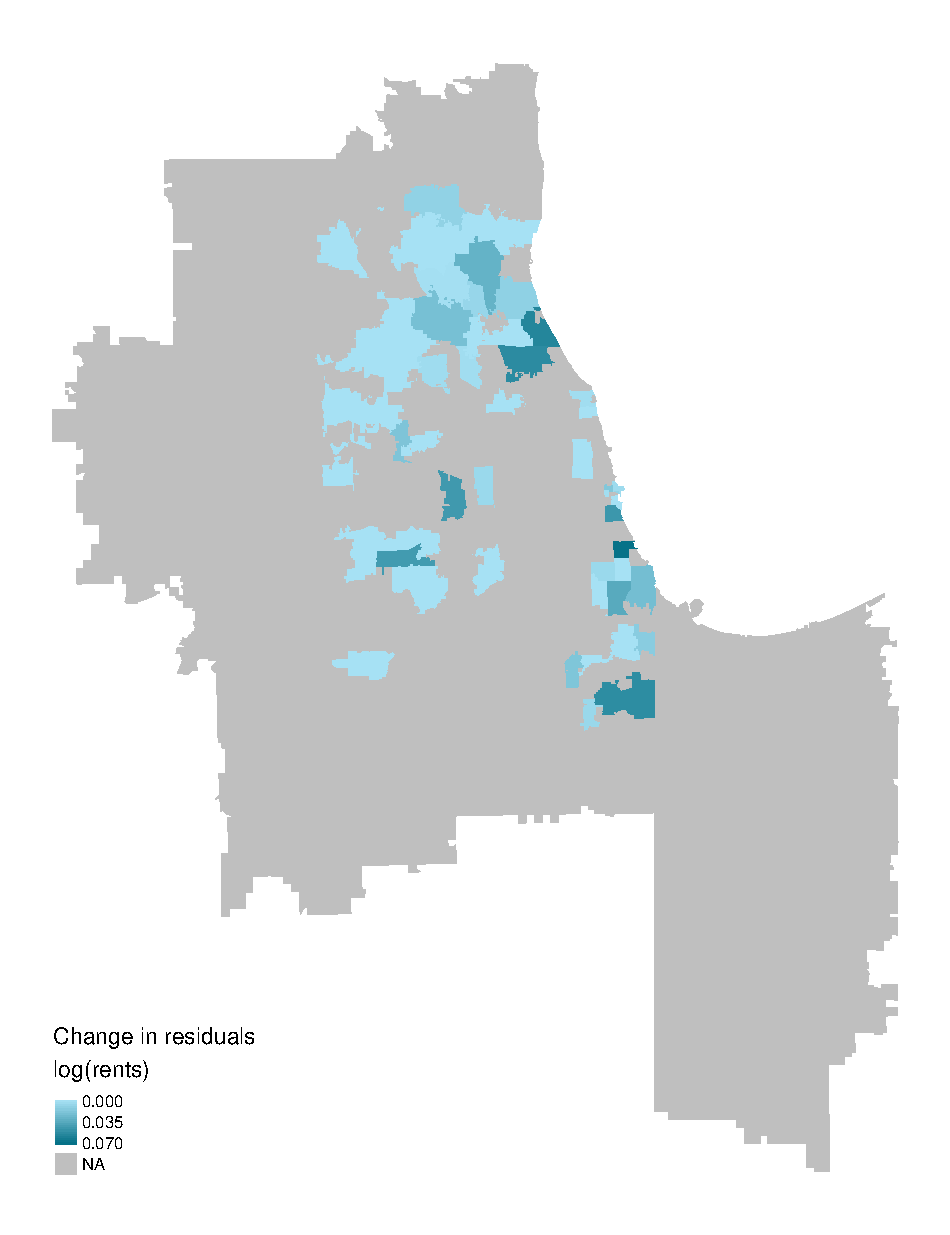
\includegraphics[width = 1\textwidth]
            {maps_events/output/chicago2019-6_r_rents}
    \end{subfigure}

    \begin{minipage}{.95\textwidth} \footnotesize
        \vspace{3mm}
        Notes: 
        Data are from the unbalanced estimation panel described in Section
        \ref{sec:data_final_panel}.
        Panel (a) maps the residuals of a regression of the change in the 
        workplace MW measure on the change in the residence MW measure, 
        including economic controls and year-month fixed effects.
        Panel (b) maps the residuals of a regression of the change in log 
        rents on economic controls and year-month fixed effects.
        The residence MW is defined as the log statutory MW in the same ZIP code.
        The workplace MW is defined as the statutory MW where the average 
        resident of the ZIP code works, constructed using LODES 
        origin-destination data.
        Economic controls from the QCEW include the change of the following 
        variables: the log of the average wage, the log of employment, and the 
        log of the establishment count for the sectors ``Information,''
        ``Financial activities,'' and ``Professional and business services.''
    \end{minipage}
\end{figure}

\clearpage

\begin{figure}[h!]
    \centering
    \caption{Estimates of the effect of the MW on rents, county by month data}
    \label{fig:dynamic_county_month}

	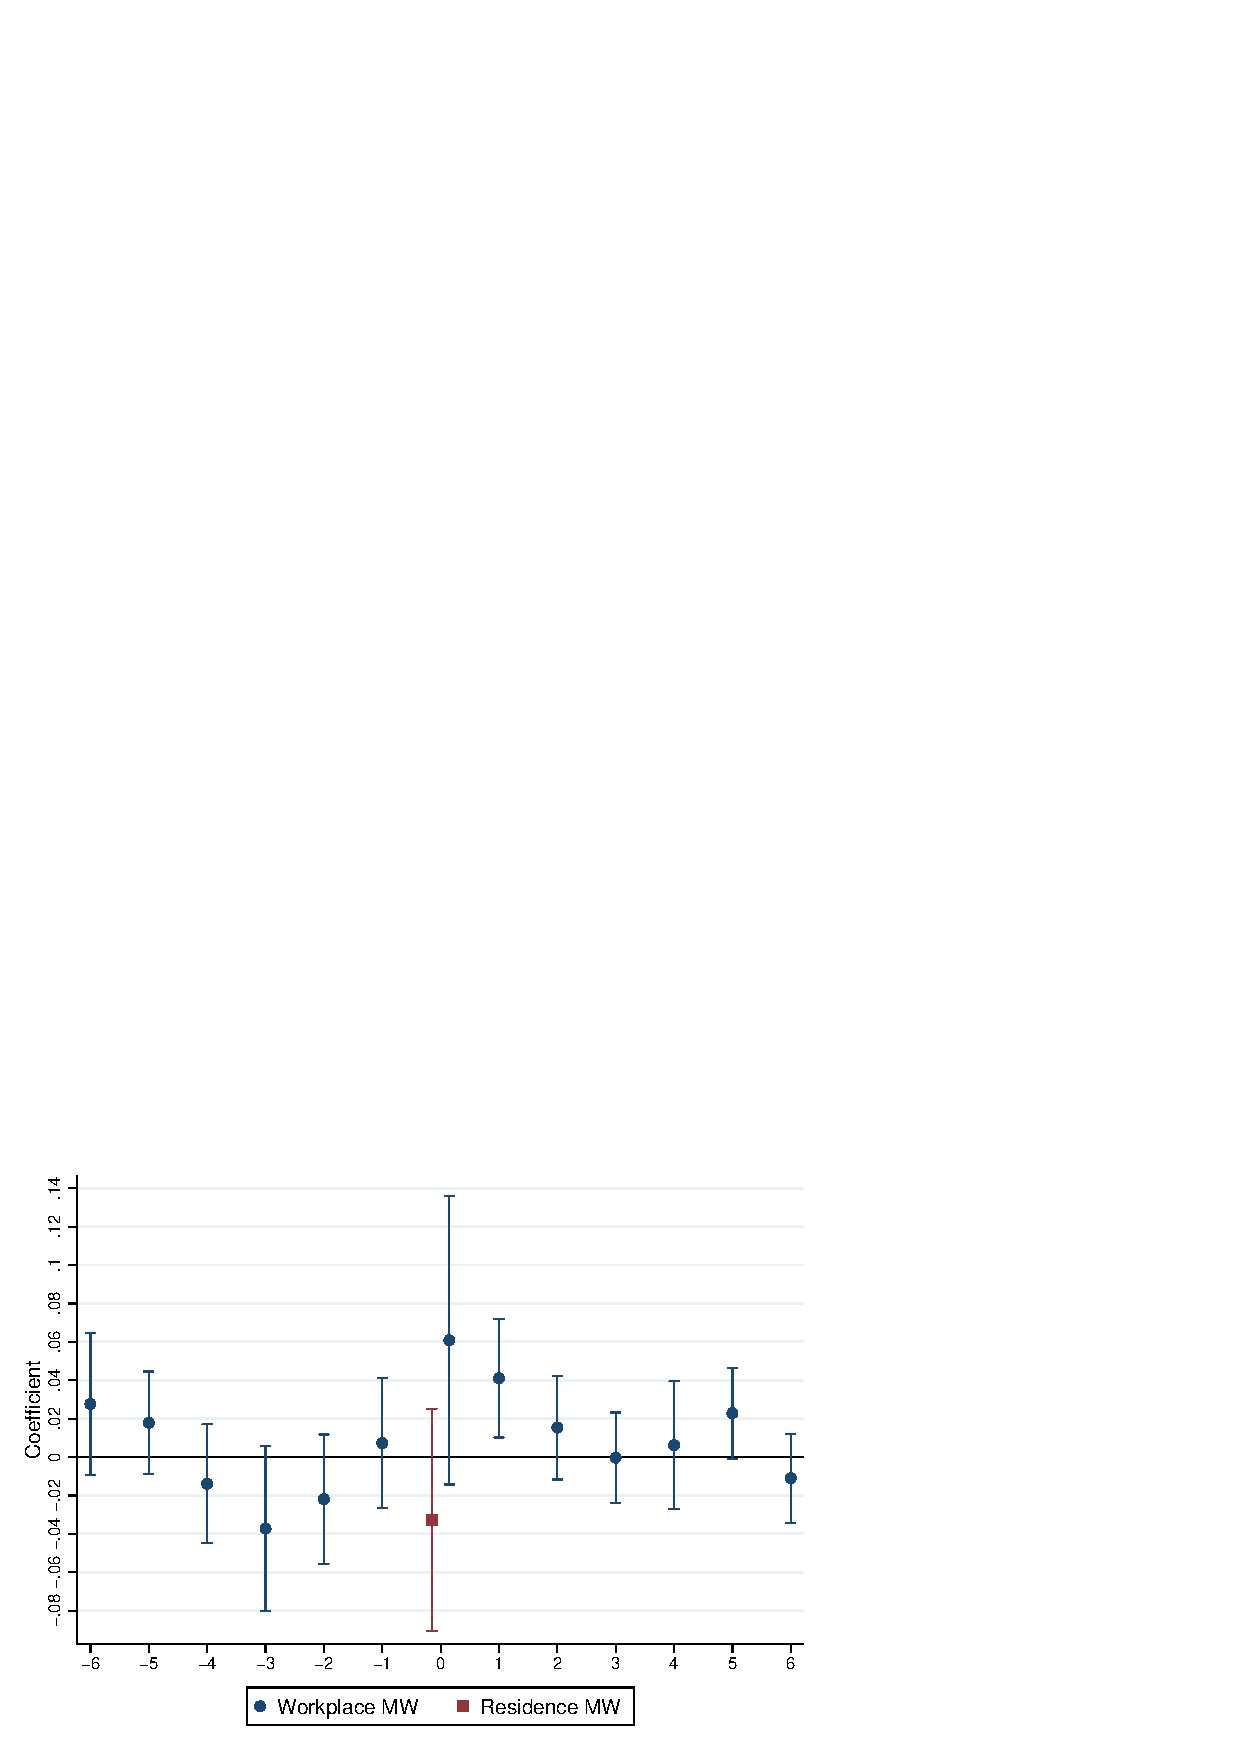
\includegraphics[width = 0.75\textwidth]{fd_geos_times/output/fd_both_mw_wkp_only_dynamic.png}

    \begin{minipage}{.95\textwidth} \footnotesize
        \vspace{3mm}
        Notes:
        Data are from the a county by month panel described in Section 
        \ref{sec:data_final_panel}.
        We plot coefficients from regressions of the log of rents per
        square foot on the residence and workplace MW measures, including 
        six leads and lags of the workplace MW measure.
        All regressions are estimated in first differences and include 
        time-period fixed effects and economic controls that vary at the 
        county and month levels.
        The measure of rents per square foot correspond to the Single Family, 
        Condominium and Cooperative houses from Zillow.
        The residence MW is defined as the log statutory MW at the County.
        The workplace MW is defined as the log statutory MW where the average 
        resident of the county works, constructed using LODES 
        origin-destination data.
        Economic controls from the QCEW include the change of the following 
        variables: the log of the average wage, the log of employment, and the 
        log of the establishment count for the sectors ``Information,'' 
        ``Financial activities,'' and ``Professional and business services.''
        95\% pointwise confidence intervals are obtained from standard errors 
        clustered at the state level.
    \end{minipage}
\end{figure}

\clearpage
\begin{figure}[h!]
    \centering
    \caption{Distribution of counterfactual increases in MW measures, 
             urban ZIP codes}
    \label{fig:cf_hist_res_and_wkp_mw}
    \begin{subfigure}{0.5\textwidth}
        \caption*{Residence MW}
        \includegraphics[width = 1\textwidth]{counterfactuals/output/hist_d_mw_res.png}
    \end{subfigure}%
    \begin{subfigure}{0.5\textwidth}
        \caption*{Workplace MW}
        \includegraphics[width = 1\textwidth]{counterfactuals/output/hist_d_mw_wkp.png}
    \end{subfigure}

    \begin{minipage}{.95\textwidth} \footnotesize
        \vspace{3mm}
        Notes:
        Data are from LODES and the minimum wage panel described in Section 
        \ref{sec:data_mw_panel}.
        The figures show the distribution of changes in the residence and 
        workplace MW measures generated by a counterfactual increase to \$9 
        in the federal MW in January 2020, holding constant other MW policies 
        in their December 2019 levels.
        The unit of observation is the urban ZIP code, where we define a ZIP code 
        as urban if it belongs to a CBSA with at least 80\% of its population 
        classified as urban by the 2010 Census.
    \end{minipage}
\end{figure}

\clearpage
\begin{figure}[h!]
    \centering
    \caption{Changes in Chicago-Naperville-Elgin CBSA due to a counterfactual raise 
    	     of the federal MW to \$9 in January 2020}
    \label{fig:map_chicago_cf_wkp_res}
    
    \begin{subfigure}{.49\textwidth}
        \caption*{Changes in residence MW}
        \includegraphics[width = 1\textwidth]
            {counterfactuals/output/chicago_d_mw_res.png}
    \end{subfigure}%
    \begin{subfigure}{.49\textwidth}
        \caption*{Changes in workplace MW}
        \includegraphics[width = 1\textwidth]
            {counterfactuals/output/chicago_d_mw_wkp.png}
    \end{subfigure}

    \begin{minipage}{.95\textwidth} \footnotesize
        \vspace{3mm}
        Notes: 
        Data are from LODES and the minimum wage panel described in Section 
        \ref{sec:mw_construction}.
        The figures maps changes in the residence and workplace MW measures 
        generated by a counterfactual increase to \$9 in the federal MW in 
        January 2020, holding constant other MW policies in their December 2019 
        levels.
    \end{minipage}
\end{figure}



\end{document}
